\abstract{A Cognitive Radio (CR) system aims at an efficient utilization of the spectrum below $\SI{6}{GHz}$ -- suitable for mobile communications -- by enabling a secondary access to the licensed spectrum while ensuring a sufficient protection to the licensed users. Despite the fact that an extensive amount of literature has been dedicated to the field of CR, its performance analysis has been dealt inadequately from a deployment perspective. Therefore, making it difficult to understand the extent of vulnerability caused to the primary system. %Motivated by this fact, this thesis establishes a deployment-centric viewpoint for analyzing the performance of a CR system. 
Following a deployment perspective, it has been identified that the involved channels' knowledge is pivotal for the realization of CR techniques. However, the aspect of channel knowledge in context of CR systems, particularly its detrimental effect on the performance, has not been clearly understood. With the purpose of curtailing this gap, this chapter proposes a successful integration of this knowledge by carrying out estimation of the involved channels within a CR system. %-- in reference to different CR systems, namely interweave, underlay and hybrid systems. 
More specifically, the chapter outlines the following two aspects: first, this chapter establishes an analytical framework to characterize the degradation in the performance due to effects such as time allocation and variation, arising due to imperfect channel knowledge. %In order to facilitate hardware deployment of a CR system, received power-based estimation, a novel channel estimation technique is employed for the channels existing between the primary and the secondary systems, thus fulfilling low-complexity and versatility requirements. Besides, this thesis follows a stochastic approach for characterizing the variations in the system. In particular, these variations cause uncertainty in the interference power received at the primary system, which may completely disrupt the operation of the CR systems. In order to maintain this uncertainty below a desired level, new interference constraints are proposed in the thesis. Moreover, the theoretical expressions, derived for the performance evaluation, are verified by means of simulations. 
Second, the chapter features performance tradeoffs that determine the maximum achievable throughput of the CR systems while satisfying the interference constraint. %At the system design, these tradeoffs provide insights for evaluating the performance degradation in terms of throughput caused due to an inappropriate selection of the estimation and sensing durations.
}

\section{Introduction}
\label{sec:Int}
% Always give a unique label
% and use \ref{<label>} for cross-references
% and \cite{<label>} for bibliographic references
% use \sectionmark{}
% to alter or adjust the section heading in the running head
Since the invention of smart devices, the mobile traffic has been increasing tremendously over the last decade. According to the recent surveys on mobile traffic by prominent market leaders (Cisco \cite{CISCO14} and Ericsson \cite{Eric15}), the existing mobile traffic is expected to increase $11$-fold  by 2021. The wireless community including the standardization bodies (3GPP) believe that the state-of-the-art standards (fourth-Generation (4G) \index{4G} -- LTE \index{LTE}, WiMAX \index{WiMAX}) are not capable of sustaining these ever-increasing demands in the upcoming decade. With this situation in hand, the standardization bodies are currently in the phase of conceptualizing the requirements of the fifth-Generation (5G) \index{5G} of mobile wireless systems.
Some of these major requirements are: (i) areal capacity in $\SI{}{bits/sec/m^2}$ must increase by a factor of $1000$ compared to 4G, (ii) low latency of approximately \SI{1}{ms}, and (iii) energy- and cost-efficient deployment \cite{Andrews14}.

The feasibility of these requirements can be envisaged through the application of promising approaches such as maximization of the spatial degrees of freedom (using techniques like massive \index{MIMO}MIMO \cite{Lar14} and 3D-beamforming \cite{Hal13}), in-band full duplex communications \index{CR communication!in-band full duplex} \cite{Sab14}, small cell densification \cite{Andrews12, Gel13}, alternatives to the already allocated spectrum -- such as millimeter-Wave technology (mmW) \cite{Rapp13}, visible light communications \cite{Wu14} and Cognitive Radio (CR) communications -- and waveform design \cite{Scha14}. A classification of these approaches is described in \figurename~\ref{fig_Int:5G}. In order to narrow down the perspective, in this chapter, a deployment scenario that lays emphasis on the small cell densification and the implementation of CR is proposed. Before proceeding further, it is essential to briefly discuss some of the prerequisites that render small cell densification and CR communication approaches, particularly their combination, a suitable candidate for a 5G network.

\begin{figure}[b]
\centering
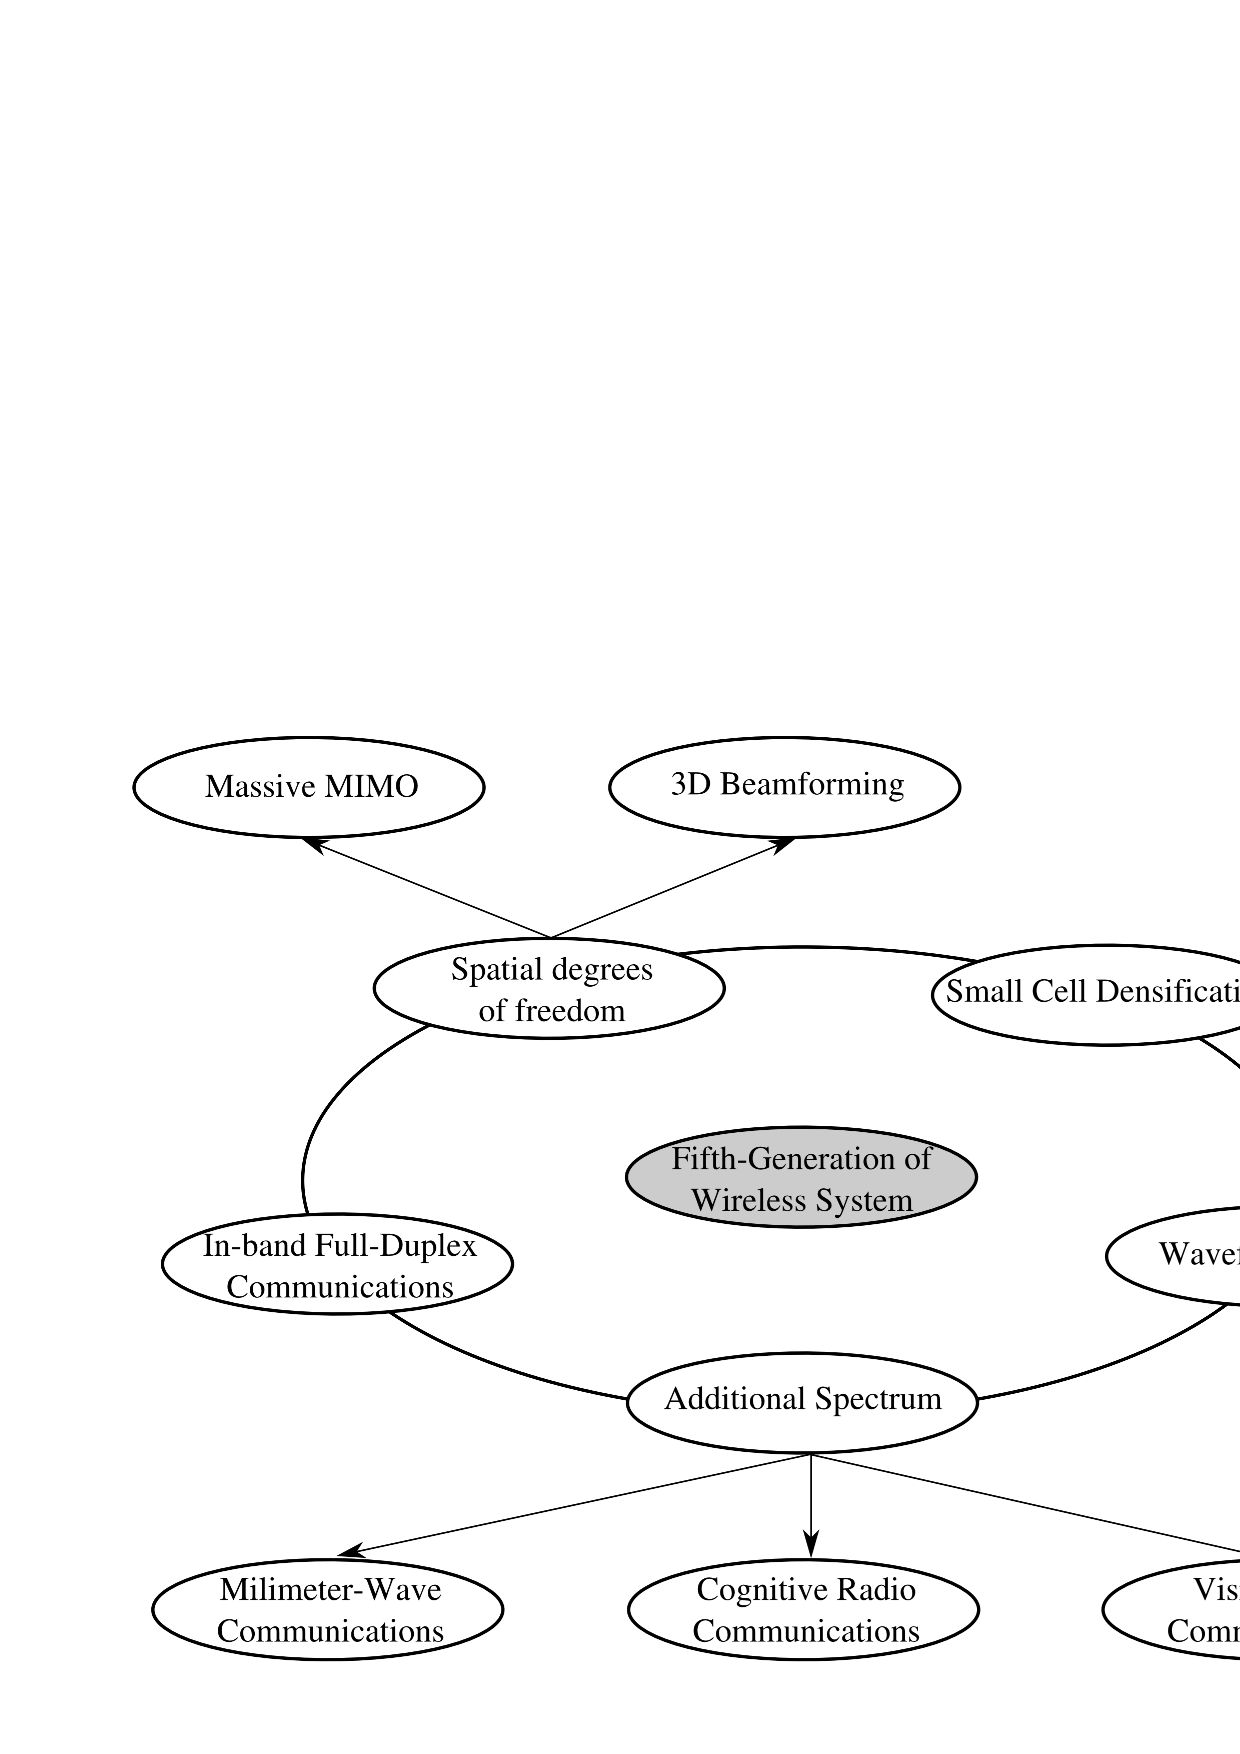
\includegraphics[width = \figfscale]{figures/5G}
\caption{An illustration of the potential approaches considered under the 5G framework.}
\label{fig_Int:5G}
\end{figure}

\subsubsection*{Small Cell Densification \index{Small cell densification}}

In the recent past, Small Cells (SCs) have emerged as a potential solution for coverage and capacity enhancements inside a wireless network. An SC represents a low power station that ranges from $\SI{10}{m}$ to $\SI{100}{m}$. The reduced transmit distance accomplished with the deployment of SCs enhances the link quality and aids spatial reuse \cite{Chander08}.
%SC is particularly deployed in a indoor or outdoor environments, these include enterprise, shopping complex or residential \cite{SSF14}. 
As a result, small cell densification can leverage the areal capacity of a 5G network \cite{Andrews14}. Because the capacity increases linearly with the number of SCs, it is infeasible to procure the factor of $1000$ in the areal capacity with densification alone. In addition, the operation and the integration of these substantial number of SCs to the backhaul network are cost- and energy-intensive for the mobile operator. Therefore, the degree to which the densification can be achieved by a wireless network is rather limited.

\subsubsection*{Additional Spectrum\index{Additional Spectrum}}
Complementing the SCs, an additional spectrum %\footnote{The spectrum corresponds to the radio frequency.} 
is envisioned as a power source that is capable of sustaining the desired areal capacity for 5G. In consideration to the present allocation of the spectrum below $\SI{6}{Hz}$ to different wireless services, it is difficult to procure an extension to the already available spectrum to the mobile communication. Before investigating the potential candidates for the spectrum extension, it is necessary to consider the following classification of the spectrum:
%\begin{itemize}
(i) $> \SI{6}{GHz}$;
(ii) $\le \SI{6}{GHz}$.
%\end{itemize}
This sort of classification allow us to focus on the feasibility characteristics and the issues thereof.


The spectrum beyond \SI{6}{GHz} largely entails the mmW\index{Millimeter-wave technology}, which is well-known for point-to-point communications. Recently, it is envisaged as a powerful source of spectrum for 5G wireless systems. However, the mmW technology is still in its initial stage and along with complex regulatory requirements in this regime, it has to address several challenges like propagation loss, low efficiency of radio frequency components such as power amplifiers, small size of the antenna and link acquisition \cite{Rapp13}. Therefore, in order to capture a deeper insight of its feasibility in 5G, it is essential to overcome the aforementioned challenges in the near future.%\nociteK{Kaushik13, Kaushik14_W, Kaushik14_CC, Kaushik14_P, Kaushik15_CC,Kaushik15_ICC, Kaushik15_D, Kaushik16_TWC, Kaushik16_VTC1, Kaushik16_TCCN, Kaushik16_ICC, Kaushik16_CC, Kaushik16_VTC2, Kaushik17}

\begin{figure}[!t]
\centering
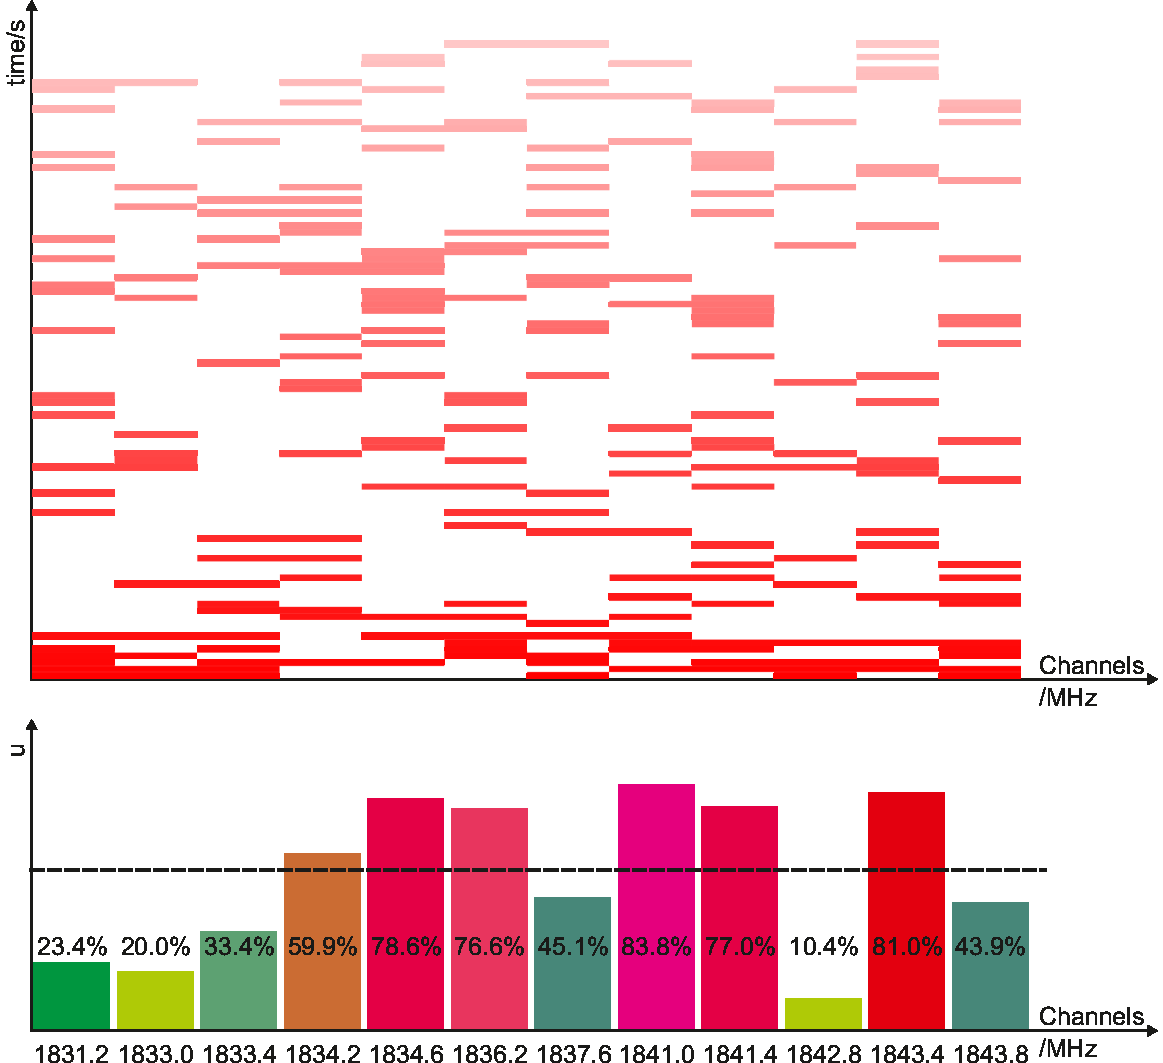
\includegraphics[width = \figscalett]{figures/Grafik_Poster}
\caption{A snapshot of a hardware demonstrator that measures the spectral occupancy in \index{GSM}GSM \SI{1800}{MHz} downlink channels, whereby the red slices represent the spectrum occupancy (1 or 0) corresponding to a single measurement at a given time instant. The bar plots illustrate the spectrum occupancy (u) for each channel with a history of 500 measurements \protect\cite{Kaushik13}.}
\label{fig_Int:HW_I}
\end{figure}
In contrast to the spectrum beyond \SI{6}{GHz}, an efficient utilization of the spectrum below \SI{6}{GHz} presents an alternative solution. The use of the spectrum in this regime (below \SI{6}{GHz}) is fragmented and statically allocated \cite{Mchen05, Mchen07}, leading to inefficiencies and the shortage in the availability of the spectrum for new services. A glimpse of the measurement campaign demonstrating the underutilized spectrum is presented in \figurename~\ref{fig_Int:HW_I}. The measurements, acquired during the peak hours, illustrate the spectrum occupancy for the GSM \SI{1800}{MHz} downlink sub-channels. The low spectrum occupancy for most of the sub-channels clearly signifies the fact that the demand for the additional spectrum can be fulfilled only by managing the utilization of the available spectrum efficiently.

In this perspective, CR is foreseen as one of the potential contenders that addresses the spectrum scarcity problem. Since its origin by Mitola \textit{et al.} in 1999 \cite{Mitola99}, this notion has evolved at a significant pace, and consequently has acquired certain maturity. Despite the existence of the theoretical analysis, from a deployment perspective, this technology is still in its preliminary phase \cite{Pawe11}. In order to curtail the gap between the theoretical models and the practical implementations, recently, the wireless community has started to show an inclination towards models and/or techniques as indicated by the increased promotion of hardware implementation/demonstration or the events such as spectrum challenge \cite{Kaushik15_D} in conferences like IEEE DySPAN. Hence, facilitating a hardware implementation of this concept in a way encourages the disposition of CR systems in the upcoming 5G wireless systems. Motivated by this fact, this chapter focuses on the performance analysis of CR systems from a deployment perspective.

In contrast to the Radio Frequency (RF) spectrum, Visible Light Communication (VLC) \index{Visible light communication} has started to gain extensive attention for 5G wireless communication, hence, deserves consideration in context to spectrum extension. Despite the fact that VLC offers some attractive characteristics like spatial, spectrum reuse, high energy efficiency and security, it has to overcome certain challenges such as mobility and adverse effect of atmospheric conditions while operating outdoor \cite{Wu14}.

In order to enhance the readability, this chapter is organized as follows: Sect.~\ref{sec:CS} features different CR systems. Next, to illustrate a successful incorporation of the CR in a 5G network, a specific use-case (deployment scenario) is presented subsequently in Sect.~\ref{sec:CSC}. Sect.~\ref{sec:PA} brings out the key aspects that are pivotal to performance analysis of a CR system. Sect.~\ref{ssec:ICK} underlines the significance channel knowledge with regard to the realization of CR techniques on a hardware platform. It also describes the harmful effects arising due to the imperfect channel knowledge, leading to performance degradation. In order to justify this argument, Sect.~\ref{sec:IS} presents a case study that incorporates channel estimation to characterize the performance of CR as interweave system. %In this regard, Sect.~\ref{sec:IS} develops an analytical framework that includes the estimation of the involved channels in accordance with the interweave scenario. 
Thus, the indoor deployment scenario is transformed into an interweave scenario, whereby a spectrum sensing mechanism is employed at the CSC-BS enabling a secondary access to the licensed spectrum. In addition, this section establishes an analytical framework to capture the effect of imperfect channel knowledge on the performance. %It further characterizes an estimation-sensing-throughput tradeoff that depicts the suitable estimation and the suitable sensing time intervals at which the maximum secondary throughput is achieved by an IS. 
Sect.~\ref{sec:RD} presents some possible direction for further research. Finally, Sect.\ref{sec:Con} concludes the chapter.  Table \ref{tb:tb1} lists the definitions of acronyms and important mathematical notations used throughput the chapter. 
 
\begin{table}
%\vspace{-0.4cm}
\renewcommand{\arraystretch}{1.4}
\caption{Definitions of Acronyms and Notations used}
%\vspace{-0.6cm}
\label{tb:tb1}
\centering
%\scriptsize{
%\begin{tabular}{l||l}
\begin{tabular}{p{0.25\columnwidth}||p{0.6\columnwidth}}
\hline
\bfseries Acronyms and Notations & \bfseries Definitions \\
\hline\hline
AC, OC & average constraint, outage constraint \\ \hline
%AWGN & Additive White Gaussian Noise  \\ \hline
CR & cognitive radio\\ \hline
CSC, CSC-BS, MC-BS, MS & cognitive small cell, cognitive small cell-base station, macro cell-base station, mobile station\\ \hline
IM, EM & ideal model, estimation model \\ \hline
IS & interweave system \\ \hline
PU - PT, PR & primary user - primary transmitter, primary receiver \\ \hline
SU - ST, SR & secondary user - secondary transmitter, secondary receiver \\ \hline
$\mathcal H_1, \mathcal H_0$ & Signal plus noise hypothesis, noise only hypothesis\\ \hline
$\fsam$ & Sampling frequency\\ \hline
$\test, \tsen$ & Estimation time, sensing time interval\\ \hline
$T$ & Frame duration\\ \hline
$\pd, \pfa$ & Detection probability, false alarm probability \\ \hline
$\pdd$ & Target detection probability\\ \hline
$\mpd$ & Outage constraint over detection probability\\ \hline
$\hpo, \hpt, \hs$ & Channel coefficient for the link PT-ST, PT-SR, ST-SR \\ \hline
$\snrrcvd, \snrso$ & Signal to noise ratio for the link PT-ST, ST-SR \\ \hline
$\snrpt$ & Interference (from PT) to noise ratio for the link PT-SR \\ \hline
$\rs$ & Throughput at SR\\ \hline
$\cz,\co$ & Date rate at SR without and with interference from PT  \\ \hline
$\mu$ & Threshold for the energy detector\\ \hline
$F_{(\cdot)}$ & Cumulative distribution function of random variable $(\cdot)$\\ \hline
$f_{(\cdot)}$ & Probability density function of random variable $(\cdot)$\\ \hline
$\hat{(\cdot)}$ & Estimated value of ($\cdot$)\\ \hline
$\tilde{(\cdot)}$ & Suitable value of the parameter ($\cdot$) that achieves maximum performance \\ \hline
$\mathbb E_{(\cdot)}$ & Expectation with respect to ($\cdot$) \\ \hline
$\p$ & Probability measure \\ \hline
\textbf{T}$(\cdot)$ & Test statistics\\ \hline
%$x_{(\cdot)}[n], y_{(\cdot)}[n]$ & $n\supe{th}$ sample of the transmitted discrete and real signal, received discrete and real signal at ($\cdot$) \\ \hline
%$P\sub{Tx, $(\cdot)$},  P\sub{Rx, $(\cdot)$}$ & Power transmitted, power received at ($\cdot$) \\ \hline
$\spo,  \npo$ & Signal variance at PT, noise variance at ST and SR\\ \hline
%$\Gamma(\cdot)$ & Gamma function\\ \hline
%$\Gamma(\cdot, \cdot)$ & Regularized incomplete upper Gamma function\\ \hline
%$\Gamma^{-1}(\cdot, \cdot)$ & Inverse of regularized incomplete upper Gamma function\\ \hline
%$\mathcal N, \cchi2, \ncchi2$ & Normal, central chi-squared, non-central chi-squared distribution\\ \hline
%$ \Ks$ & Number of pilot symbols used for pilot based estimation at the SR for $\hs$ \\ \hline
%$ \Kp$ & Number of samples used for received power based estimation at the SR for $\hpt$ \\ \hline
%$\as,
%$\ls$ & Non-centrality parameter of  $\ncchi2$ distribution \\ \hline
\end{tabular}
%}
\end{table}
 

\section{Cognitive Radio Systems \index{Cognitive radio systems!classification}}
\label{sec:CS}
In order to proceed further, it is essential to understand the classification of different CR systems described in the literature. An access to the licensed spectrum is an outcome of the paradigm employed by a Secondary User (SU). In this context, all CR systems that provide shared access (used interchangeably with secondary access) to the spectrum mainly fall under the following categories \cite{Goldsmith09}, please consider \figurename~\ref{fig_Int:paradigm} for a graphical illustration of different CR systems, including some specific CR techniques. 
\begin{itemize}
\item According to Interweave System (IS) \index{Interweave system!definition}, the SUs render an interference-free access to the licensed spectrum by exploiting spectral holes in different domains such as time, frequency, space and polarization.
\item An Underlay System (US) \index{Underlay system!definition} enables an interference-tolerant access, according to which the SUs are allowed to use the licensed spectrum (e.g. Ultra Wide Band (UWB)) as long as they respect the interference constraints of the Primary Receivers (PRs).
\item A Hybrid System (HS) \index{Hybrid system!definition} combines the benefits of the IS (agility to detect spectrum holes in different domains) and the US (interference-tolerant capability) so that the spectrum available for performing secondary access can be used efficiently.
\item An Overlay system \index{Overlay system!definition} considers advanced transmission and coding strategies, which include the participation of higher layers for enabling the spectral coexistence between two or more wireless networks.
\end{itemize}
The IS, the US and the HS are closely associated with the physical layer, hence, these systems are mostly considered not only for the theoretical analysis but for practical implementations as-well \cite{Kaushik13, Kaushik14_CC, Kaushik15_D, Kaushik16_CC, Kaushik16_VTC2, Cabric04, Cabric06, Kim10}. 
Underlying this fact, this chapter establishes a deployment-centric viewpoint towards these CR systems. In order to illustrate a successful incorporation of the CR in a 5G network, a specific use-case (deployment scenario) is presented subsequently.


\begin{figure}
\centering
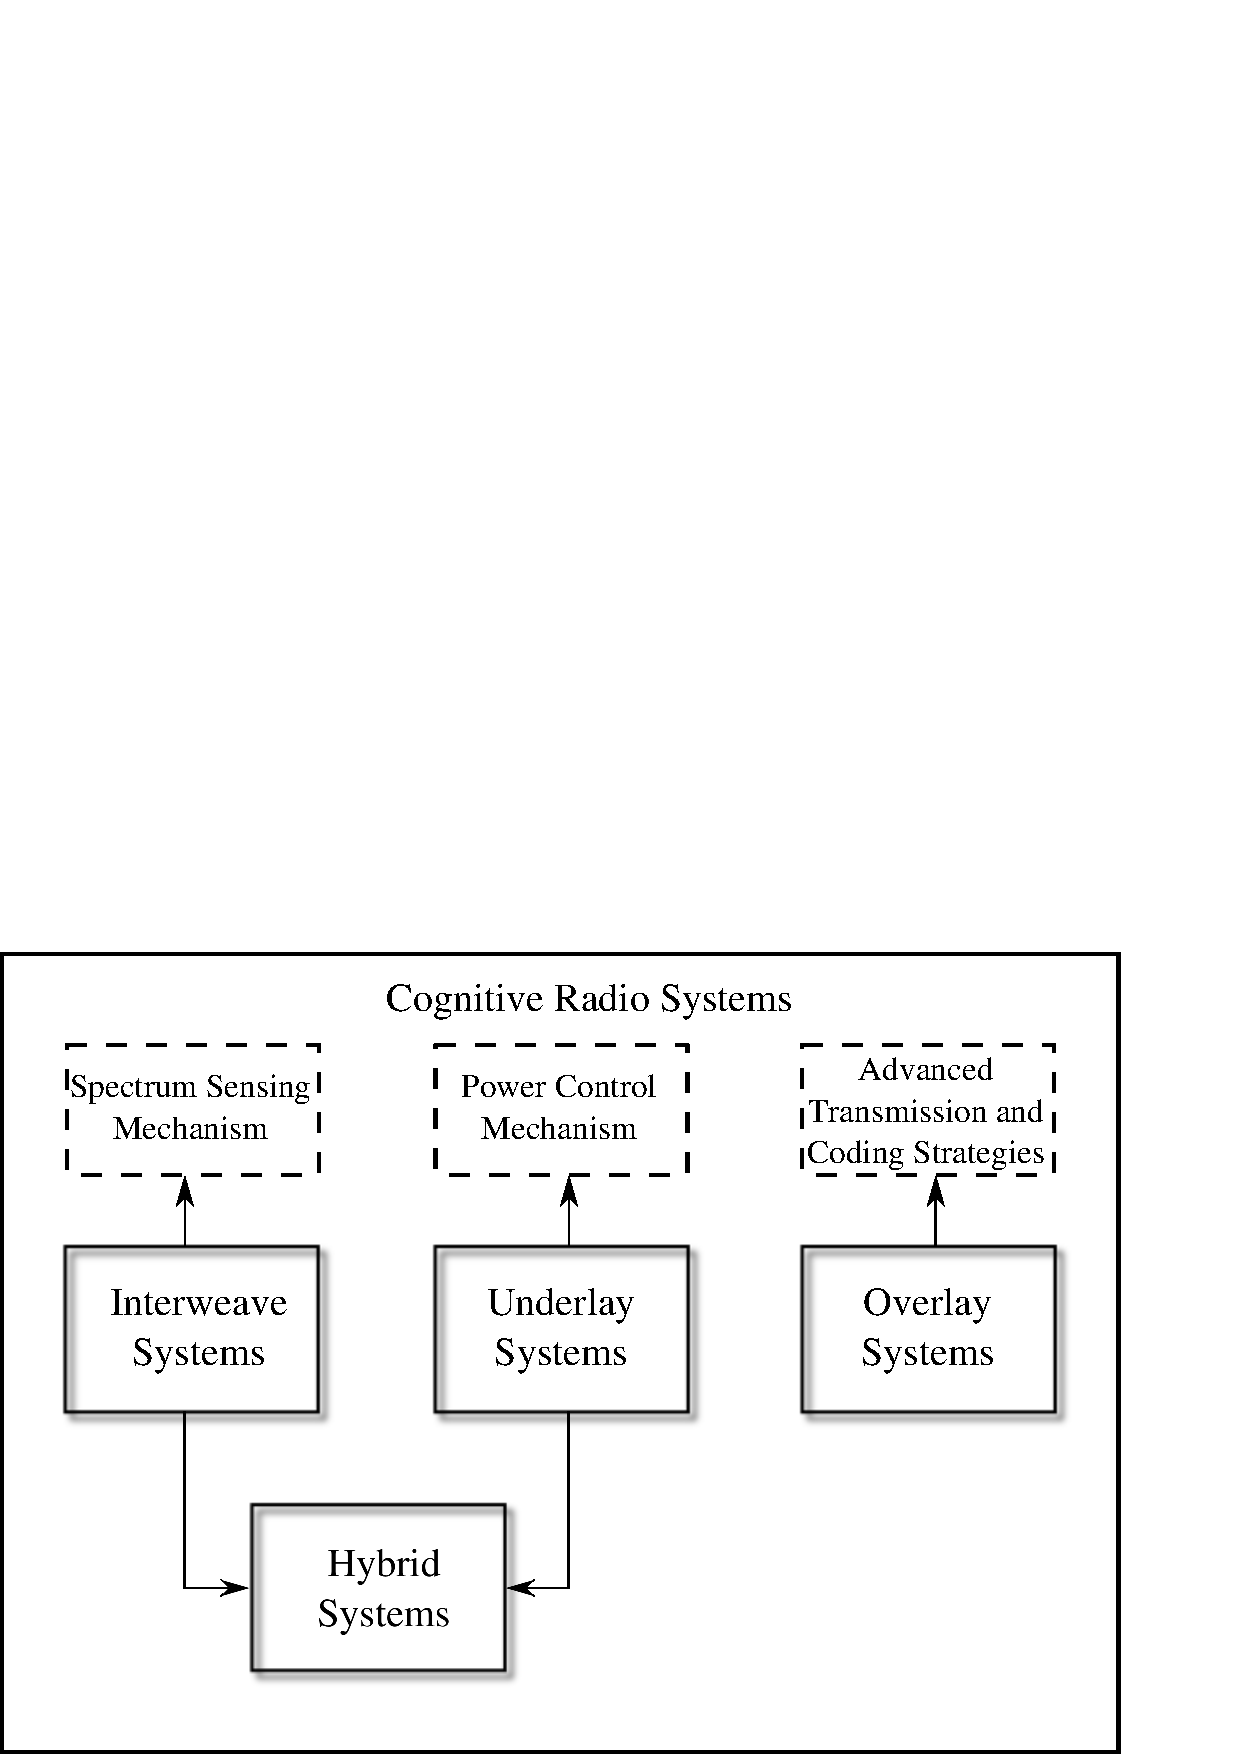
\includegraphics[width = 0.85 \columnwidth]{figures/CR_paradigm}
\caption{A classification of different CR systems and some specific CR techniques that allow shared access to the licensed spectrum.}
\label{fig_Int:paradigm}
\end{figure}


\section{Cognitive Small Cell: A Prominent Use-Case}
\label{sec:CSC}
\begin{figure}
\centering
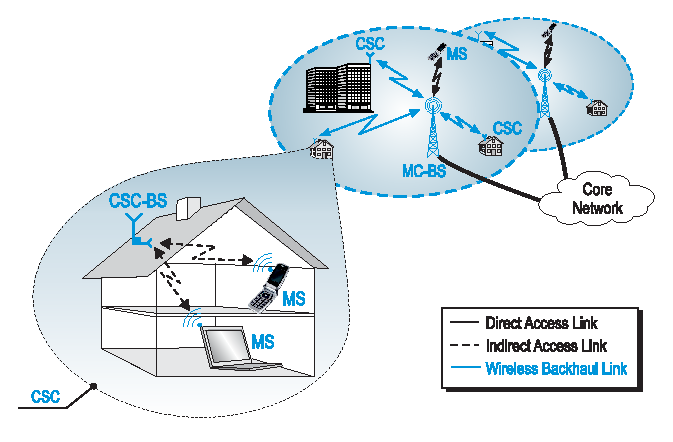
\includegraphics[width = 0.8 \columnwidth]{figures/Cellular_Scenario_CR_T6}
\caption{An illustration of the CSC deployment in a 5G network.}
\label{fig_Int:archi}
\end{figure}

It is evident from the previous discussion in Sect.~\ref{sec:Int} that the spectrum extension via CR systems and SC densification are significant to the \index{5G}5G system. %Recently, ElSawy \textit{et al.} \cite{Elsawy13} have presented Cognitive Small Cell (CSC), a concept that fulfills the capacity demands of the future wireless networks. 
Based on this, a preliminary concept of Cognitive Small Cell (CSC), a promising application that combines the benefits from the SC deployment and the efficient usage of the spectrum below \SI{6}{GHz}, by realizing CR, is presented. A typical scenario where the CSC finds its application would be the co-existence of Wi-Fi or unlicensed small cell and wireless cellular systems \cite{Benn13}. The notion of CSC has been previously investigated by Elsawy \textit{et al.} \cite{Elsawy13_cmag}, where the authors primarily emphasized on the modeling techniques that depict the positioning of several CSCs inside the network. The modeling is based on \index{Stochastic geometry}stochastic geometry, which allows a spatial averaging over multiple network geometries \cite{Haenggi}. Due to this, the performance analysis of the CSC has been limited mainly to network abstraction. In contrast, this chapter examines the fundamental aspects encountered while deploying a CSC, which otherwise could forbid its realization of this concept over the hardware. %, which could possibly lead to a successful integration of CSCs in the 5G network. %Consequently, by considering different CR paradigms to enable secondary usage of the licensed spectrum, here a deeper comprehension of the concept is illustrated. %, thereby, making it accessible to 5G systems. 
%To strengthen our understanding of CSC, we demonstrate the feasibility of the respective paradigms by means of hardware implementations.
%Pertaining to the deployment, we analyze the true performance of the CSC as a CR application for the mentioned paradigms.  
 A comprehensive incorporation of CSC in a preliminary 5G architecture is illustrated in \figurename~\ref{fig_Int:archi}. In order to enhance the viability of the proposed network architecture, it is reasonable to highlight some of the essential ingredients pertaining to the deployment of the CSC.


\subsection{Network Elements \index{Cognitive small cell!network elements}}
 In order to propose a successful integration of CSC in a 5G network, the following key elements are essential: a CSC-Base Station (CSC-BS), a Macro Cell-Base Station (MC-BS) and Mobile Stations (MSs), cf. \figurename~\ref{fig_Int:archi}. MSs are the devices either served by the MC-BS over a \textit{direct access} link or the CSC-BS over an \textit{indirect access} link. The direct access and the indirect access are the nomenclature used to distinguish a start-of-the-art (spectrum) access between the MC-BS and the MS from an access between the CSC-BS and the MS representing a CR communication, respectively. Furthermore, the MC-BS is connected to several CSC-BSs over a \textit{wireless backhaul} link. Although the MC-BS and the MS already exist in the conventional cellular architecture, to incorporate the opportunistic access inside the CSC, it is necessary to consider a functionality upgrade.

\subsection{Spectrum Access\index{Cognitive small cell!spectrum access}}
In the proposed network architecture, the access to the spectrum is realized over the wireless backhaul, the direct access and the indirect access links, cf. \figurename~\ref{fig_Int:archi}.
\begin{enumerate}
\item A wireless backhaul is a
%quasi-line of sight\footnote{It allows limited number of objects between the direct link.} 
point-to-point wireless link between the CSC-BS and the MC-BS that relays the traffic generated from the CSC to the core network. With regard to the densification of the CSC in 5G network, the wireless backhaul link, in contrast to the optical fiber link, presents a cost-effective and energy-efficient alternative to the mobile operator.
With limited infrastructure required for the deployment, wireless backauling accelerates the installation process and promotes scalability of the network.
For the wireless backhaul link, considering that it is utilized for a longer time duration, an exclusive spectrum represents a viable option. In this context, it is sensible to nominate a mmW band; alternatively, an exclusive band below \SI{6}{GHz} can be acquired using the principles of \index{LSA}Licensed Shared Access (LSA) \cite{ETSI13}.
%These WB links encourage ultra-densification as they brings down the capital expenditure and offer scalability to the vendor. 

\item A direct access link represents a direct access of the MS at the MC-BS over the allocated spectrum. Consequently, the spectrum access for this link is analogous to the one existing in the state-of-the-art wireless standards.
\item The CSC elements (the CSC-BS and the MS) are responsible for executing the secondary access to the licensed spectrum. The additional spectrum, acquired through the realization of CR techniques, \index{CR techniques}including spectrum sensing and power control, at the CSC-BS, is used for the communication between the CSC-BS and the MS over the indirect access link.
\end{enumerate}

\subsection{Hardware Feasibility\index{Cognitive small cell!hardware feasibility}}
Along with other ingredients, it is essential to outline certain aspects that pertain to the hardware realizability of the CSC. For the CSC-BS, an antenna mount system consisting of an indoor and an outdoor antenna is proposed. Whereby, the indoor antenna exploits the walls of the building to physically separate the indoor transmissions over the indirect access link. In this way, the CSC is able to mitigate the interference to the primary system and to the neighbouring CSCs, vice-versa. Whereas, the outdoor antenna secures a narrow beam transmission to enhance the link quality for the wireless backhaul link. Besides this, it is a well-known fact that Software Defined Radio \index{SDR}(SDR) has played an important role in the genesis of the CR \cite{Jondral05}. This means that the SDR can serve as a suitable platform for executing CR techniques, accomplishing rapid prototyping for the CR systems. Taking this into account, the SDR platform is utilized for realizing (or demonstrating) the CR functionality pursued by the CSC-BS over a hardware.


\subsection{Indoor Deployment\index{Cognitive small cell!indoor deployment}}
From a market survey, it has been depicted that $70\%$ of the mobile traffic is originated from indoor locations \cite{Chander08}. Another survey of the leading \index{WiMAX}WiMAX operators revealed that $80\%$ of their subscribers will be connected indoors \cite{Pao07}. In addition, a new range of wireless services, categorized as Internet of Things (IoT), will operate indoors. Following these facts, it is clear that the performance gains in terms of spectrum reuse will be far more consequential if we manage to consolidate these sources of traffic by means of SCs deployment. In order to capture the indoor originated traffic, it is sensible to consider the residential and enterprise as the main deployment scenarios for the CSC, cf. \figurename~\ref{fig_Int:archi}. Except for a different coverage regime, the operating principles of these scenarios are analogous. Besides, in context with the CR, where the interference mitigation between the primary and the secondary systems is a significant aspect, a CR communication within walls (which attributes to an indoor deployment) provides a spatial separation between the two systems. This, however, does not indicate that CR communication is limited to indoor scenarios. As the matter of fact, the indoor deployment is opted \begin{itemize} \item to exploit the behavioral dimension of the traffic source (traffic management) and \item to mitigate the interference between the two systems \end{itemize} so that co-existence with the licensed users is encouraged.
In this regard, an indoor scenario is considered for the deployment of the CSC, cf. \figurename~\ref{fig_Int:archi}. Besides employing such interference mitigation approach, an effective control over the interference is essential for a successful operation of the CR systems. Therefore, the next section extensively discusses the performance of the CR systems.


\section{Performance Analysis of CR Systems: A Challenging Task}
\label{sec:PA}
Since the evolution of wireless systems, understanding the performance of novel algorithms/techniques related to the wireless systems has always been a challenging task. With regard to this, for a CR system, because of the involvement of two different systems, namely primary and secondary systems, this task is even more difficult. On one end, it has been engaging a large number of researchers that are eager to find solutions for the new set of problems that are emerging from an interplay between these two systems, leading them to develop theoretical models (system models). As a result, these models allow us to determine the performance limits of the CR system. However, to sustain analytical tractability, they tend to consider assumptions that in most situations are unrealistic for a hardware deployment.  %However, with the lack of concrete guidelines, different perspective have forward for the performance analysis.
 
On the other end, due to the co-existence of the two systems sharing the same spectrum, the performance of a CR system is critical to the regulatory bodies and the mobile operators, responsible for managing the spectrum. These operators are the ones who are willing to share their license (as primary system) or the ones who are willing to access the licensed spectrum (as secondary system). In this regard, despite the numerous theoretical models that exist in the literature, when it comes to judging the performance of a CR system, the regulatory bodies give more preference to the hardware implementations. 

These different mindsets and the lack of proper guidelines ultimately slow down the evolution of the CR in realistic scenarios. Under this situation, it is advisable to merge these mindsets and establish a deployment-centric viewpoint towards the CR systems, according to which the upcoming models and/or techniques not only associate themselves to the performance characterization but also eligible for practical implementations. %This viewpoint, also the main motivation behind this work, is emphasized throughout the thesis.

The co-existence between the primary and the secondary systems can be accomplished only through a detailed analysis of the performance of these systems. %The lack of proper guidelines defining these systems and their co-existence leave the performance analysis of the CR systems a challenging task. 
To address this issue, the researchers have made an intensive effort to develop system models \cite{Liang08, Kang209, Kang09} that characterize the performance of the CR systems. The performed analysis boils down to the fact that the CR systems are allowed to successfully co-exist with the primary system only if they respect the interference power (or interference) at the primary system caused due to an access to the licensed spectrum. In other words, imposing an interference constraint ensures a sufficient protection to the primary systems and enables the CR system to perform secondary access.

\begin{figure}
\centering 
\tikzstyle{every node}=[draw=black,thick,anchor=west]
\tikzstyle{selected}=[draw=red,fill=red!30]
\tikzstyle{optional}=[dashed,fill=gray!50]
\begin{tikzpicture}[%
  grow via three points={one child at (0.5,-0.7) and
  two children at (0.5,-0.7) and (0.5,-1.4)},
  edge from parent path={(\tikzparentnode.south) |- (\tikzchildnode.west)}]
  \node {Imperfections (or Uncertainties)}
    child { node {Noise Uncertainty}}	
    child { node {Channel Imperfections}}
    child { node {Signal Uncertainty}}
    child { node {Channel/Noise Correlation}}
    child { node {Hardware Imperfections}
      child { node {RF Distortions}}
      child { node {Synchronization Errors}}
      child { node {Quantization Errors}}
    }
    child[missing] {}  
    child[missing] {}  
    child[missing] {}  
    child { node {Modeling Imperfections}
      child { node {Signal Modeling}}
      child { node {Signal Pre-processing}}
      %child { node {Parameter Estimation}}
      child { node {Channel Fading}}
    }
;
\end{tikzpicture}
\label{fig:imp}
\caption{An illustration of major imperfections (or uncertainties) in CR systems \cite{Sharma15}.} 
\end{figure}

With regard to the aforementioned constraint, the CR system also intends to deliver a certain Quality of Service/Quality of Experience (QoS/QoE) in the form of throughput to its corresponding Secondary Receiver (SR), defined as \index{Secondary throughput}\textit{Secondary throughput}. Such a QoS/QoE provisioning helps us to determine the potential applications or prominent use-cases for the CR system. For instance, the secondary throughput's knowledge over the access link enables the CR to execute a band allocation policy, based on which the CR can relinquish those channels that ineffectively contribute to the secondary throughput, and/or are responsible for causing interference at the primary system. As a result, the performance of a CR system can be jointly characterized in terms of the harmful interference received at the primary system and the throughput achieved by the secondary system.

But the fact is, the derived expressions depicting the performance of the CR systems are rarely examined over the hardware. Mainly, because of the complicated deployment scenario or the computational complexity of the employed CR techniques, leaving the validity of the existing theoretical analysis questionable. Because of this, we tend to overlook certain imperfections (or uncertainties) inherent to the CR systems, including noise uncertainty, channel imperfections, signal uncertainty, noise/channel correlation, hardware imperfections and modeling imperfections \cite{Sharma15}, which may be responsible for degrading the performance of CR systems, refer to \figurename~\ref{fig:imp}. In other words, by neglecting these imperfections in the system model, the performance of a CR system is overestimated. To narrow down the perspective, this chapter considers the effect on performance of CR systems due to imperfect channel while putting emphasis on the fact that the performed analysis can be easily validated through a hardware implementation.


\subsection{Imperfect Channel Knowledge}
\label{ssec:ICK}
In a nutshell, \textit{a CR is an agile system that possesses the ability to adapt to the changes in the environment}. From a physical layer perspective, this corresponds to the response to the changes incurred within the system or from the outside environment, which in a way leads to a performance enhancement. Inherent to the wireless systems, these changes may arise due to the variations in the signal caused by the presence of the thermal noise at the receiver and the fading in the channel. It is well-known from the text-books, related to wireless communications \cite{Goldsmith05, Tse05}, that the channel fading, in particular, is critical for wireless systems. As a matter of fact, channel knowledge -- in the form of Channel State Information at the Transmitter \index{CSIT}(CSIT) available through a feedback from the receivers -- has rendered a substantial improvement in the performance in terms of data rate, for instance, multiplexing gains for a \index{MIMO}MIMO system \cite{Ali12}.


%\begin{figure}[!t]
%\centering
%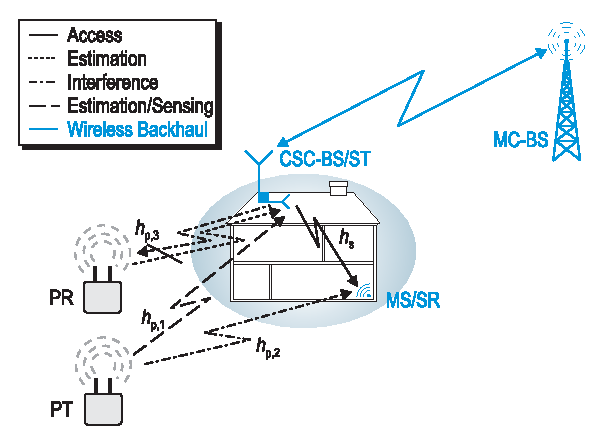
\includegraphics[width = \figscale]{figures/CR_Scenario_Hybrid}
%\caption{A cognitive small cell scenario demonstrating: (i) the CR systems employed at the CSC-BS, (ii) the associated network elements, which constitute Cognitive Small Cell-Base Station/Secondary Transmitter (CSC-BS/ST), Mobile Station/Secondary Receiver (MS/SR), Macro Cell-Base Station (MC-BS) and Primary Transmitter (PT), (iii) the interacting channels: sensing ($\hpo$), interference ($\hptw, \hpth$) and access ($\hs$) channels.}
%\label{fig_Int:scenario}
%\vspace{-6mm}
%\end{figure}


In context with a CR system, the channel knowledge, unlike the conventional or state-of-the-art wireless systems, is not confined to a single transmitter-receiver link. It rather includes all the related channels that exist within as-well-as across the primary and the secondary systems. Therefore, at this stage, it is worth understanding the fact that channel knowledge is paramount for the hardware implementation of the CR systems. This knowledge allows them to exercise CR techniques and to respect the desired interference constraints, which are necessary for their co-existence with the primary systems. Besides, from a theoretical perspective, the channel knowledge is required for the performance characterization. Absence of this knowledge, especially of those channels that are related to the interference at the primary systems, renders the performance characterization of a CR system inadequate for the practical implementations.


Despite the existence of multitude of analytical models in the literature \cite{Liang08, Sharma14, Ghasemi07} that consider with the performance analysis of a CR system, its performance with regard to the channel estimation, due to the complexity of the underlying problem, has never been completely understood. In order to curtail this gap, this chapter capitalizes on the estimation of the involved channels in a CR system. In this sense, the accessibility of the channel knowledge at the CSC-BS facilitates the implementation of the CR techniques at the CSC-BS, establishing a CR communication link with the MS over the acquired spectrum. More importantly, this knowledge allows us to regulate the interference at the PR below a desired level.

Certainly, an access to the channel knowledge comes at a certain cost. Firstly, the inclusion of channel estimation demands an allocation of a certain time interval by the CSC-BS. In consideration to the time allocation, a certain degradation in the performance in terms of the throughput is obvious. Secondly, the variations introduced due to the estimation process, also treated as imperfect channel knowledge, lead to an uncertainty in the interference, defined as \index{Uncertain interference}\textit{uncertain interference}, to the primary systems. The uncertain here specifically symbolizes the variations in the interference power received at the PR that exists because of the imperfect channel knowledge. If not considered, this uncertain interference may severely degrade the performance of the CR systems. In order to approach a successful integration of channel estimation into the CR system, it is essential to consider the performance degradation arising due to the time allocation and the uncertain interference in the system model. These effects concerning the performance degradation have been completely left aside in the existing models that consider the perfect channel knowledge. Sect.~\ref{sec:IS} takes these effects into account to establish analytical frameworks that allow us to understand the behaviour of the CR systems as interweave systems under those situations that are close to realistic scenarios. %Subsequently, these frameworks are utilized to characterize the performance of the respective CR systems.

Shifting the focus back to the deployment, it is worthy to understand that the channel estimation, facilitating shared access to the licensed spectrum, is viable only if the CR system is equipped with the knowledge about to the primary system. %In this way, the CR system is dependent on the wireless standard followed by the primary system. 
This implies that in order to perform channel estimation based on conventional techniques -- such as training-based \cite{Stoica03}, pilot-based \cite{Gifford05, Gifford08}, signal to noise ratio-based \cite{Chav11, Sharma13} channel estimation, which already exist in the literature -- a preliminary processing in the form of synchronization and demodulation of the baseband signal received from the primary system is necessary. The existence of multiple wireless standards and their complexity preclude us from deploying a dedicated circuitry corresponding to each primary system \cite{Ghasemi08_cm}. The fact is, these conventional channel estimation techniques are well-known for delivering accurate channel estimates, that is why employed in state-of-the-art wireless standards. However, in context of the CR systems, these techniques \begin{itemize} \item increase the complexity related to the channel estimation, evaluated in terms of the mathematical operations, and (or) \item demand the demodulation of the Primary User (PU) signal. \end{itemize}

Under these circumstances, it is advisable to consider only those solutions that offer low complexity and show versatility towards different PU signals. Generally speaking, such solutions will not only ease the deployment process but also have a large acceptance among the CR community. For instance, energy-based detection (or energy detection) has been a popular choice compared to its counterparts such as matched filtering-based and cyclostationary-based detection for detecting a PU signal, required for performing spectrum sensing for the interweave systems (discussed later in Sect.~\ref{sec:IS}). A direct comparison of these techniques by simply counting their implementations for hardware demonstration has been done in \cite{Pawe11}.

On similar grounds as energy detection, in order to approach the channel estimation for the CR system, particularly for the channels that involve the primary systems, a \textit{received power-based}\index{Channel estimation!received power-based}
channel estimation technique is proposed as a part of the analytical framework. It is worthy to understand that the received power refers to the signal power measured after analog to digital conversion, hence, it consists of the signal and the noise power. Traditionally, received signal strength is a metric used for measuring signal quality to perform tasks such as cell association and handover \cite{Boga16}. This channel estimation technique is introduced to substitute the conventional techniques because, like energy detection, employing received power-based estimation assures the low complexity and the versatility towards unknown PU signal requirements of the CR system, and consequently facilitates its deployment. Besides, the channel within the secondary framework, treated as a conventional transmitter-receiver link, does not fall in the aforementioned category. Therefore, its knowledge is procured by employing a pilot-based channel estimation technique\index{Channel estimation!pilot-based}.



\subsection{Modeling Imperfections}
Besides imperfect channel knowledge, this section briefly discusses some key issues that are necessary from a deployment perspective, but left aside while establishing the system model. 

\subsubsection{Signal Modeling}
The Gaussian and the constant power signals are generally used for modeling the PU signals, which correspond to Orthogonal Frequency Division Multiplexing (OFDM) and Phase Shift Keying (PSK) modulated signals, respectively. In practice, this modeling can be employed only if the sampling point is selected appropriately, hence resulting in i.i.d. samples. In other situations, the samples are correlated.
%Besides sampling point, several components in the RF chain, such as filtering, also introduce a certain amount correlation between the samples. 
This correlation is not considered while modeling the system, hence leads to deviation of the performance parameters (false alarm probability and detection probability) obtained theoretically from the ones obtained by performing the measurements. In order to resolve this issue, the OFDM and PSK modulated signals can be replaced with their mathematical counterparts for signal transmission, these include a Gaussian and a sinusoidal signal, respectively. By doing this, we are able to avoid the correlation between the samples that are used for computing the energy.

\subsubsection{Signal Pre-processing}
\begin{figure}
        %\vspace{-10 pt}
        \centering
        \subfloat[Signal with oversampling, where the local oscillator is tuned at $\flo = \SI{50}{kHz}$]
        {
                \begin{tikzpicture}[scale=1]
                \node[anchor=south west,inner sep=0] (image) at (0,0)
                {

                        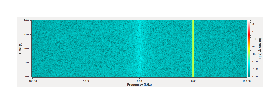
\includegraphics[width=0.9\textwidth]{figures/Spektrum}
                };
                \begin{scope}[x={(image.south east)},y={(image.north west)}]
                \draw[black,thick,<->] (0.498,0.98) --  node[above, font=\footnotesize] {$\flo = \SI{50}{kHz}$} (0.718,0.98);
                \draw[white, dashed] (0.4,0.155) rectangle node[above, font=\footnotesize, text width = 2cm, align=center] {\textcolor{white}{DC offset and flicker noise}} (0.6,0.942);

                %\draw[help lines,xstep=.1,ystep=.1] (0,0) grid (1,1);
                %\foreach \x in {0,1,...,9} { \node [anchor=north] at (\x/10,0) {0.\x}; }
                %\foreach \y in {0,1,...,9} { \node [anchor=east] at (0,\y/10) {0.\y}; }
                \end{scope}
                \end{tikzpicture}
                \label{fig_HVD:SP_os}
        } \\
        \subfloat[Signal after bandpass filtering, filter bandwidth  $= \SI{50}{kHz}$]
        {

                \begin{tikzpicture}[scale=1]
                \node[anchor=south west,inner sep=0] (image) at (0,0)
                {

                        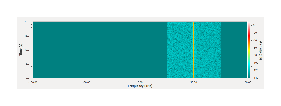
\includegraphics[width=0.9\textwidth]{figures/bpf}
                };
                \begin{scope}[x={(image.south east)},y={(image.north west)}]
                \draw[black,thick,<->] (0.605,0.98) --  node[above, font=\footnotesize] {Band pass filter = $\SI{50}{kHz}$} (0.825,0.98);

                %\draw[help lines,xstep=.1,ystep=.1] (0,0) grid (1,1);
                %\foreach \x in {0,1,...,9} { \node [anchor=north] at (\x/10,0) {0.\x}; }
                %\foreach \y in {0,1,...,9} { \node [anchor=east] at (0,\y/10) {0.\y}; }
                \end{scope}
                \end{tikzpicture}
                \label{fig_HVD:SP_bp}
        } \\
        \subfloat[Signal after digital downconversion]
        {
                
\includegraphics[width=0.9\textwidth]{figures/runtergemischt}
                \label{fig_HVD:SP_dc}
        } \\
        \subfloat[Signal after decimation]
        {
                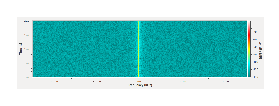
\includegraphics[width=0.9\textwidth]{figures/dezimiert}
                \label{fig_HVD:SP_de}
        }
        %\vspace{-10 pt}
        \caption{An illustration of the signal processing steps carried out at the host computer to preclude the spurious effects such as the DC offset and the flicker noise on the signal received at the ST.}
        \label{fig_HVD:SP}
\end{figure}


Generally, ST is emulated using an SDR platform (for instance, Universal Software Radio Peripheral \index{USRP}(USRP) B210, an SDR from Ettus Research \cite{Ettus}). Such low-cost hardwares are associated with a direct downconversion of the bandpass to the baseband signal -- a homodyne receiver -- spurious effects such as DC offset, flicker noise $(1/f)$ and I/Q imbalance arising from the analog front-end can affect the accuracy of the analytical expressions. These spurious effects, particularly the DC offset and the flicker noise, become significant at low signal to noise ratio. In order to retrieve the complex samples close to the one obtained while characterizing the system model that do not take such spurious effects into account, the following signal processing (referred as pre-processing) is proposed, please consider \figurename~\ref{fig_HVD:SP}:
\begin{itemize}
\item The received PU signal (a complex sinusoid) is oversampled with sampling frequency of $200$ $\SI{}{kHz}$.
%Now, for a bandpass filter with bandpass frequency of $\SI{50}{KHz}$ applied subsequently, this sampling corresponds to a oversampling factor = 4. 
In order to filter out the spurious effects\index{Pre-processing}, the local oscillator is tuned at a certain offset frequency defined as $\flo = \SI{50}{kHz}$, refer to \figurename~\ref{fig_HVD:SP_os}.
\item Subsequently, a bandpass filter with bandwidth = $\SI{50}{kHz}$, corresponding to a oversampling factor = $4$, is employed to obtain the desired bandpass signal at the $\flo$. This filters out the DC offset and the flicker noise present at low frequencies, cf. \figurename~\ref{fig_HVD:SP_bp}.
\item In order to obtain the lowpass equivalent of the desired signal, a digital downconversion (i.e., multiplying with a complex sinusoid with frequency $\flo = \SI{50}{kHz}$) of the bandpass filtered signal is performed, cf. \figurename~\ref{fig_HVD:SP_dc}. %These four steps depicted in \figurename~\ref{fig_HVD:SP} are carried out to remove the receiver's DC offset and the flicker noise (1/f) around the DC. Due to the small bandwidth of the pilot signal, these effects form the bottleneck of our validation and had to be accounted for. 
\item Lastly, a decimation filter (with decimation factor = 4) over the downconverted signal is applied, cf. \figurename~\ref{fig_HVD:SP_de}, to reduce the correlation between the samples, arising due to oversampling.
\end{itemize}

%\subsubsection{Parameter Estimation}
%\label{ssec:est}
%Following the characterization of the $P_{\text{d}}$ in (\ref{eq:pfapd_sls}) and (\ref{eq:pfapd_slc}) for the considered techniques, it is noticed that the knowledge of the receiver SNR $\bar{\gamma}_l$ (which is assumed to be perfectly known in the theoretical analysis) at the ST is essential. In this regard, as proposed in \cite{Kaushik16}, received power estimation for each antenna is employed. Therefore, a certain time interval $\tau_\text{est}$ within the sensing time is allocated to the SNR estimation. Upon estimating $\bar{\gamma}_l$, it is possible to evaluate the detection probability for the deployed hardware. Table \ref{tb:snr} presents the averaged (computed over different channel realizations of the channel for each antenna) value of the received SNR at each antenna for the different signal models.

\subsubsection{Channel Fading}
Channel fading is essential to establish a macroscopic view towards the performance of a CR system. With regard to this, Rayleigh block fading is mostly preferred for modeling channel fading. However, block fading considers uncorrelated over the different energy measurements. However, in practice, either uncorrelated fading is not encountered or the measurements may converge to a different fading model such as Nakagami-$m$ fading model \cite{Kaushik14_CC}. Due to this issue, hardware validation of the analytical expressions that incorporates channel fading models is rarely considered. %In order to facilitate the preliminary validation process, we propose the following simplification: The experiments are performed using a coaxial cable and Rayleigh fading is emulated at the PT.

One possible way of resolving this issue is to emulate fading at the ST, according to which the transmit signal is modulated with channel gains at the PT using software \cite{Kaushik16_VTC2}. This allows us to establish a close relation between the analytical model and the acquired energy measurements, which consequently enhances the validation of a CR system that incorporates channel fading for the performance analysis. However, to proceed with the hardware validation pertaining to scenarios that involve channel fading, in future, it is essential to incorporate correlated fading model into the system and estimate the related parameters \cite{Kaushik14_CC}. 

\section{Interweave System: A Case Study}
\label{sec:IS}
At this stage, it is well-understood that the knowledge of the related channels is crucial for the application of CR techniques in the practical scenarios. This section capitalizes on the successful integration of this knowledge on interweave system. In this context, the indoor deployment scenario is transformed into an interweave scenario, whereby a spectrum sensing mechanism is employed at the CSC-BS enabling a secondary access to the licensed spectrum. Section \ref{sec_IS:ana} derives the theoretical expressions to capture the effect of imperfect channel knowledge on the performance of an IS. Further, Section \ref{sec_IS:num_ana} establishes an estimation-sensing-throughput tradeoff that depicts the suitable estimation and the suitable sensing time intervals at which the maximum secondary throughput is achieved by an IS. Please note that this section contains material from the following publication \cite{Kaushik16_TWC}.

For detecting a PU signal, several techniques such as\index{Spectrum sensing!energy detection} energy-based detection (or energy detection), \index{Spectrum sensing!detection techniques}matched filtering-based, cyclostationary-based and feature-based detection exist \cite{Axell12}. Because of its versatility towards unknown PU signals and its low computational complexity, energy detection has been extensively investigated in the literature \cite{Urkowitz, Herath09}. In this technique, the decision is accomplished by comparing the power received at the ST to a decision threshold. In reality, the ST encounters variations in the received power due to the existence of thermal noise at the receiver and fading in the channel. Subsequently, these variations lead to sensing errors described as misdetection and false alarm, %The characterization of sensing errors as detection probability and false alarm probability has been studied in \cite{tan08}. 
which limit the performance of the IS. In order to determine the performance of a detector, it is essential to obtain the expressions of detection probability and false alarm probability.


In particular, detection probability is critical for IS because it protects the PR from the interference induced by the ST. As a result, the IS has to ensure that they operate above a target detection probability \cite{peh07}. Therefore, the characterization of the detection probability becomes absolutely necessary for the performance analysis of the IS. In this context, Urkowitz \cite{Urkowitz} introduced a probabilistic framework for characterizing the sensing errors, however, the characterization accounts only for the noise in the system.

To encounter the variation caused by channel fading, a frame structure has been introduced in \cite{Liang08}, \tc{assuming that the channel remains} constant over the frame duration (corresponds to a quasi-static block fading). Upon exceeding the frame duration, the system may observe a different realization of the channel. Based on this frame structure, the performance of the IS has been investigated in terms of a deterministic (corresponding to a non-random behaviour) channel \cite{Liang08, Sharma14} \index{Channel!deterministic channel} and a random channel\index{Channel!random channel} \cite{Alouini03, Herath09}. These deterministic and random behaviour of the channel illustrates a microscopic and a macroscopic view towards the performance characterization, respectively, of a CR system. \tc{In this chapter, the former approach is considered, hence, the performance is analyzed for a specific frame, i.e., for a certain (unknown) realization of the channel.} %Whereas the random channel represents that the performance is evaluated over multiple frames, i.e., the CR system observes multiple realizations of the channel. For the latter case, a fading model is employed to capture the random behaviour of the channel.}


Besides the detection probability, false alarm probability has a large influence on the throughput achieved by the secondary system. %Further, the characterization of the false alarm probability requires the knowledge of the noise power. Subject to a given uncertainty \cite{Tan08}, this knowledge can be acquired through hardware calibration. 
%\subsection{Problem Formulation}
Recently, the performance characterization of CR systems in terms of a sensing-throughput tradeoff\index{Tradeoffs!sensing-throughput tradeoff} has received significant attention \cite{Liang08, Juarez11}. According to Liang \textit{et al.} \cite{Liang08}, the ST assures a reliable detection of a PU signal by retaining the detection probability above a desired level with an objective of maximizing the throughput at the SR. In this way, the sensing-throughput tradeoff depicts a suitable sensing time interval that achieves a maximum secondary throughput. To characterize the detection probability and the secondary throughput, the system requires the knowledge of interacting channels, namely, a \textit{sensing} channel, an \textit{access} channel and an \textit{interference} channel, \tc{refer to} \figurename~\ref{fig_IS:scenario}. Since the interference to the PR is controlled by a regulatory constraint over the detection probability, in this view, the interaction with the PR is excluded in the considered scenario \cite{Liang08}. The baseline models, investigated in the literature, assume the knowledge of these channels to be available at the ST.
However, in practice, this knowledge is not available, thus, it needs to be estimated by the secondary system. As a result, the existing solutions for the IS are considered inadequate from a practical viewpoint.


As a matter of fact, the sensing and the interference channels related to the CR system (refer to \figurename~\ref{fig_IS:scenario}) represent the channels between two different (primary and secondary) systems. In this context, it becomes challenging to select the estimation methods in such a way that low complexity and versatility (towards different PU signals) requirements are satisfied. These issues, discussed later in Sect.~\ref{ssec_IS:pa}, render the existing estimation techniques \cite{Stoica03, Gifford05, Gifford08, Chav11, Sharma13} unsuitable for hardware implementations.
%Existing works assume it to be known at the ST. In reality, due to  this knowledge is not available at the ST. 
%The channel, regarded as deterministic and unknown, is expected to remain constant over a frame duration, 
To tackle the issue related to the channel estimation, as discussed previously in Sect.~\ref{ssec:ICK}, a received power-based estimation at the ST and at the SR for the sensing and the interference channels is employed, respectively.
Considering the fact that the access channel corresponds to the link between the ST and the SR, conventional channel estimation techniques such as pilot-based channel estimation at the ST is employed.

Inherent to the estimation process, the variations due to the channel estimation translate to the variations in the performance parameters, namely detection probability and secondary throughput. In particular, the variations induced in the detection probability cause uncertain interference at the PR, which may severely degrade the performance of a CR system. The detrimental effect due to the time allocation for the channel estimation and the uncertain interference due to imperfect channel knowledge have not been considered in \cite{Liang08, Juarez11} or studied partially in \cite{Chav11, Cao14}. In this context, the performance characterization of an IS with imperfect channel knowledge remains an open problem.
Motivated by this fact, this section focuses on the performance characterization of the IS in terms of sensing-throughput tradeoff taking these aforementioned aspects into account.


%%%%%%%%%%%%%%%%%%%%%%%%%%%%%%%%%%%%%%%%%%%%%%%%%%%%%%%%%%%%%%%%%%%%%%%%%%%%%%%%%%%%%%%%%
\subsection{System Model} \label{sec_IS:sys_mod}
%%%%%%%%%%%%%%%%%%%%%%%%%%%%%%%%%%%%%%%%%%%%%%%%%%%%%%%%%%%%%%%%%%%%%%%%%%%%%%%%%%%%%%%%%
\subsubsection{Interweave Scenario}
\index{Interweave system!involved channels}
\begin{figure}[!ht]
\centering
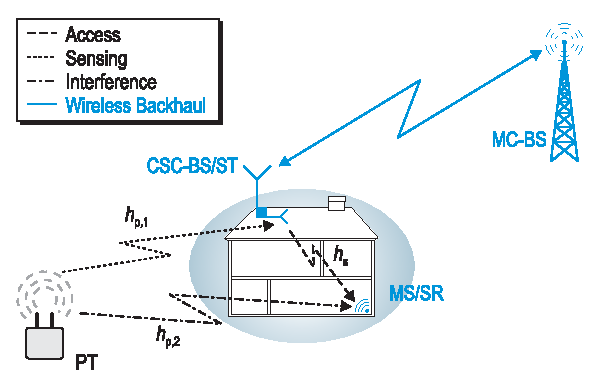
\includegraphics[width = \figscale]{figures/CR_Scenario_Interweave}
\caption{A cognitive small cell scenario demonstrating: (i) the interweave paradigm, (ii) the associated network elements, which constitute cognitive small cell-base station/secondary transmitter (CSC-BS/ST), mobile station/secondary receiver (MS/SR), macro cell-base station (MC-BS) and primary transmitter (PT), (iii) the interacting channels: sensing ($\hpo$), access ($\hs$) and interference ($\hpt$).}
\label{fig_IS:scenario}
%\vspace{-0.3cm}
\end{figure}

To consider the applicability of IS, the CSC, a CR application illustrated in the previous chapter, is transformed into an interweave scenario. Considering the fact that the IS is employed at the CSC-BS, the CSC-BS and the MS represent the ST and the SR, respectively. A hardware prototype of the CSC-BS operating as IS was presented in \cite{Kaushik13}. For simplification, a PU constraint based on false alarm probability (Neyman-Pearson criterion) was considered in \cite{Kaushik13}. With the purpose of improving system's reliability, the analysis is extended to employ a PU constraint on the detection probability.

\subsubsection{Signal Model}
%According to interweave system, ST considers a hypothesis testing to determine the presence ($\mathcal{H}_1$) or absence $(\mathcal{H}_0)$ of a signal transmitted by the PR. 
Subject to the underlying hypothesis that illustrates the presence $(\mathcal{H}_1)$ or the absence ($\mathcal{H}_0$) of a PU signal, the discrete and complex signal received at the ST is given by\index{Spectrum sensing!energy detection}
\begin{equation}
\yrcvd[n] = 
\begin{cases}
\hpo \cdot \xp[n] + \wst[n] & : \mathcal{H}_1 \\
\wst[n] & :\mathcal{H}_0
\end{cases},
\label{eq_IS:sys_mod_p1s}
\end{equation}
\tc{The signal $\xp[n]$ transmitted by the PUs} can be modeled as: (i) a PSK \index{Phase Shift Keying} modulated signal, or (ii) a Gaussian signal. The signals that are prone to high inter-symbol interference or entail precoding, for instance OFDM\index{OFDM} signal with linear precoding, can be modeled as Gaussian signals \cite{Liang08}. In this chapter, the analysis is focused on the latter case, i.e., the primary and the secondary systems employ OFDM to carry out their transmission. 
%In contrast, Chapter \ref{chap:US} associated with the US, considers the former case for the analysis. 
As a result, the mean and the variance for the signal and the noise are determined as $\e{}{\xp[n]} = 0$, $\e{}{\wst[n]} = 0$, $\e{}{|\xp[n]|^2} = \spo$ ($= \ptranpt$) and $\e{}{|\wst[n]|^2} = \npo$. The channel $\hpo$ is considered to be independent of $\xp[n]$ and $\wst[n]$. Thus, $\yrcvd[n]$ is also an independent and identically distributed (i.i.d.) random process.

Similar to (\ref{eq_IS:sys_mod_p1s}), during data transmission, the discrete and complex received signal at the SR conditioned on the detection probability ($\pd$) and the false alarm probability ($\pfa$) is given by
\begin{equation}
\ys[n] = 
\begin{cases}
\hs \cdot \xs[n] + \hpt \cdot \xp[n] +  \wsr[n] & : 1 - \pd \\
\hs \cdot \xs[n] + \wsr[n] & : 1 - \pfa
\end{cases},
\label{eq_IS:sys_mod_ss}
\end{equation}
%and on the other side, the interference signal at the SR, transmitted by the PR follows 
%\begin{equation}
%\yp[n] = \sqrt{\gpt \cdot \apt}/ \cdot \xp[n] + w[n],
%\label{eq_IS:sys_mod_p2s}
%\end{equation}
where $\xs[n]$ corresponds to discrete and complex sample transmitted by the ST and $\wsr[n]$ is the AWGN at the SR with $\mathcal{CN}(0, \npo)$. In practice, the noise power at different network nodes (the ST, the SR and the PR) have different values. The fact is, only the signal to noise ratios  received at these nodes are affected due to these different values, which are already included in the performance analysis. For the brevity of the exposition, the noise powers at these nodes are expressed using a single notation ($\npo$). Further, $|\hs|^2$ and $|\hpt|^2$ represent the power gains for the access and the interference channels, \tc{refer to} \figurename~\ref{fig_IS:scenario}.
\subsubsection{\tc{Problem Description}}\label{ssec_IS:pd}
%\subsection{Sensing}
\tc{In accordance with the conventional frame structure}, the ST performs sensing for a duration of $\tsen$. The test statistics at the ST is evaluated as
\begin{align}
\tst = \s{\tsen \fsam}{ |\yrcvd[n]|^2} \mathop{\gtrless}_{\mathcal{H}_0}^{\mathcal{H}_1} \mu, 
\label{eq_IS:test_st}
\end{align}
where $\mu$ is the decision threshold, $\fsam$ represents the sampling frequency and $\textbf{y}$ is a vector with $\tsen \fsam$ samples. $\ts$ represents a random variable, whereby the characterization of the cdf depends on the underlying hypothesis. With regard to the Gaussian signal model, which corresponds to the OFDM signal transmitted by the PU, $\ts$ follows a central chi-squared ($\cchi2$) distribution for both hypotheses $\mathcal{H}_0$ and $\mathcal{H}_1$ \cite{Kay}. It is worthy to mention here that, by avoiding the Gaussian approximation that exists due to the application of central limit theorem\index{Central limit theorem}, thereby limiting the applicability of the considered analysis to only large sample sizes. In this context, an effort has been made to derive the theoretical expressions so that the performance analysis is valid for all sample sizes.

As a result, the detection probability\index{Spectrum sensing!detection probability} $(\pd)$ and the false alarm probability\index{Spectrum sensing!false alarm probability} $(\pfa)$ corresponding to (\ref{eq_IS:test_st}) are determined as \cite{Tan08}
\begin{align}
%\pd(\mu, \tsen, \prcvd) &= \mathcal{Q}\left( \frac{\mu - \prcvd}{ \sqrt{\frac{2}{\tsen \fsam}} \prcvd} \right),  \label{eq_IS:pd} 
\pd &= \Gamma\left( \frac{\tsen \fsam}{2}, \frac{\tsen \fsam \mu}{2 \prcvdstpt} \right),  \label{eq_IS:pd} 
\end{align}
\begin{align}
\pfa &= \Gamma\left( \frac{\tsen \fsam}{2}, \frac{\tsen \fsam \mu}{2 \npo} \right),  \label{eq_IS:pfa} 
%\pfa(\mu, \tsen) &= \mathcal{Q}\left( \frac{\mu - \npo}{ \sqrt{\frac{2}{\tsen \fsam}} \npo} \right), \label{eq_IS:pfa}
\end{align}
where $\prcvdstpt$ is the power received over the sensing channel and $\Gamma(\cdot, \cdot)$ represents a regularized upper-incomplete Gamma function \cite{grad}\index{Gamma function}.

Following the characterization of $\pfa$ and $\pd$, Liang \textit{et al.} \cite{Liang08} established a tradeoff between the sensing time and the secondary throughput $(\rs)$ subject to a target detection probability $(\pdd)$. This tradeoff\index{Tradeoffs!sensing-throughput tradeoff} is represented as
\begin{align}
\trs(\ttsen) &= \maxi_{\tsen} \rs(\tsen) \nonumber \\&= \frac{T- \tsen}{T} \bigg[ \cz (1 - \pfa) \phz +  \co (1 - \pd) \pho  \bigg], \label{eq_IS:thr_id} \\
\text{s.t.} & \text{ } \pd \ge \pdd, \label{eq_IS:thr_id_con} \\ 
\text{where } \cz &= \log_2 \left(1 + |\hs|^2 \frac{\ptranst}{\npo}\right) = \log_2 \left( 1 + \snrso \right) \label{eq_IS:Cap0},\\ 
\co &= \log_2 \left(1 + \frac{|\hs|^2 \ptranst }{|\hpt|^2 \ptranpt  + \npo} \right) \nonumber \\ \quad &= \log_2 \left(1 + \frac{|\hs|^2 \ptranst }{\prcvdsr} \right) = \log_2 \left(1 + \frac{\snrso}{\snrpt + 1}  \right), \label{eq_IS:Cap1} 
\end{align}
where $\phz$ and $\pho$ are the occurrence probabilities for the respective hypothesis, whereas $\snrrcvd$ and $\snrso$ represent the signal to noise ratios for the links PT-ST and ST-SR, respectively, and $\snrpt$ corresponds to interference (from the PT) to noise ratio for the link PT-SR. Moreover, $\ptranpt$ and $\ptranst$ represent the transmit power at the PT and the ST, whereas $\prcvdsr$ corresponds to the received power (which includes the interference power from the PT and the noise power) at the SR. In addition, $\cz$ and $\co$ represent the data rate without and with the interference from the PT. Please note, the following terms the data rate $\cz$, $\co$ and the throughput $\rs$ have been introduced to make a clear distinction between the instantaneous data rate and its average value over the frame duration. Also, the use of the term ``capacity'' is avoided for representing $\cz$ and $\co$, since it implies the optimization of the mutual information over the cognitive channel. 

In other words, using (\ref{eq_IS:thr_id}), the ST determines a suitable sensing time $\tsen = \ttsen$, such that the secondary throughput is maximized subject to a target detection probability, \tc{refer to} (\ref{eq_IS:thr_id_con}). From the deployment perspective, the tradeoff depicted above has the following fundamental issues:
\begin{itemize}
\item Without the knowledge of the received power $\prcvdstpt$ over the sensing channel, it is not feasible to characterize $\pd$, refer to (\ref{eq_IS:pd}). This renders the characterization of the secondary throughput (\ref{eq_IS:thr_id}) impossible and the constraint defined in (\ref{eq_IS:thr_id_con}) inappropriate.
\item Moreover, the knowledge of the interference and the access channels is required at the ST, \tc{refer to} (\ref{eq_IS:Cap0}) and (\ref{eq_IS:Cap1}) for characterizing the throughput in terms of $\cz$ and $\co$ at the SR.
\end{itemize}

\subsubsection{\tc{Proposed Approach}} \label{ssec_IS:pa}

\tc{In order to overcome the difficulties discussed in Sect.~\ref{ssec_IS:pd}, the following strategy is proposed.
\begin{enumerate}
\item As a first step, the estimation of the involved channels is considered. In order to characterize the detection probability, a received power-based estimation at the ST for the sensing channel is employed. This is done to ensure that the detection probability remains above a desired level. Further, a pilot-based estimation and a received power-based estimation for the access channel and the interference channel are employed at the ST and the SR, respectively, to characterize the secondary throughput. 
\item Next, the variations due to channel estimation in the estimated parameters, namely, received power (for the sensing and the interference channels) and the power gain (for the access channel) are characterized in terms of their cdfs.
\item In order to investigate the performance of the IS subject to the channel estimation, these variations in the performance parameters, which include the detection probability and the secondary throughput, are characterized in terms of their cdfs.
\item Finally, the derived cdfs are utilized to obtain the expressions of sensing-throughput tradeoff. Hence, based on these expressions, the impact of imperfect channel knowledge on the performance of the ISs is qualified, and subsequently the achievable secondary throughput at a suitable sensing time is determined.
\end{enumerate}
}
Considering the channel estimation, it is well-known that systems with transmitter information (which includes the filter parameters, pilot symbols, modulation type and time-frequency synchronization) at the receiver acquire the channel knowledge by listening to the pilot data sent by the ST \cite{Gans71, Gifford05, Gifford08, Anna05}. Other systems, where the receiver possesses either no access to this information or is limited by hardware complexity, procure channel knowledge indirectly by estimating a different parameter that entails the channel knowledge, for instance, received signal power \cite{Kaushik15_CC} or received signal to noise ratio \cite{Chav11, Sharma13}. Recently, estimation techniques such as pilot-based estimation \cite{Suraweera10, Kim12} and received power-based estimation \cite{Kaushik15_ICC} have been applied to obtain channel knowledge for the CR systems. However, the performance analysis has been limited to the underlay systems, where the emphasis has been given on modeling the interference at the PR.

Since the pilot-based estimation requires the knowledge of the PU signal at the secondary system, the versatility (in terms of PU signals) of the secondary system is compromised. On the other side, for the estimation of the received signal to noise ratio\index{Channel estimation!received signal to noise ratio-based},\index{Channel estimation!eigenvalue-based} Eigenvalue (which involves matrix operations) based approach \cite{Sharma13} or iterative approaches such as expectation-maximization have been proposed \cite{Chav11}. Due to the complicated mathematical operations or the complexity of the iterative algorithms, such approaches tend to increase the hardware complexity of the ISs. In order to resolve these issues, a received power-based estimation\index{Channel estimation!received power-based} for the sensing and the interference channels, and a pilot-based estimation\index{Channel estimation!pilot-based} for the access channel is employed. Similar to the energy based detection, since the received power-based estimation involves simple operations on the obtained samples such as magnitude squared followed by summation, the proposed estimation provides a reasonable tradeoff between complexity and versatility.


\paragraph{Frame Structure\index{Interweave system!frame structure}}
\begin{figure}[!ht]
\centering
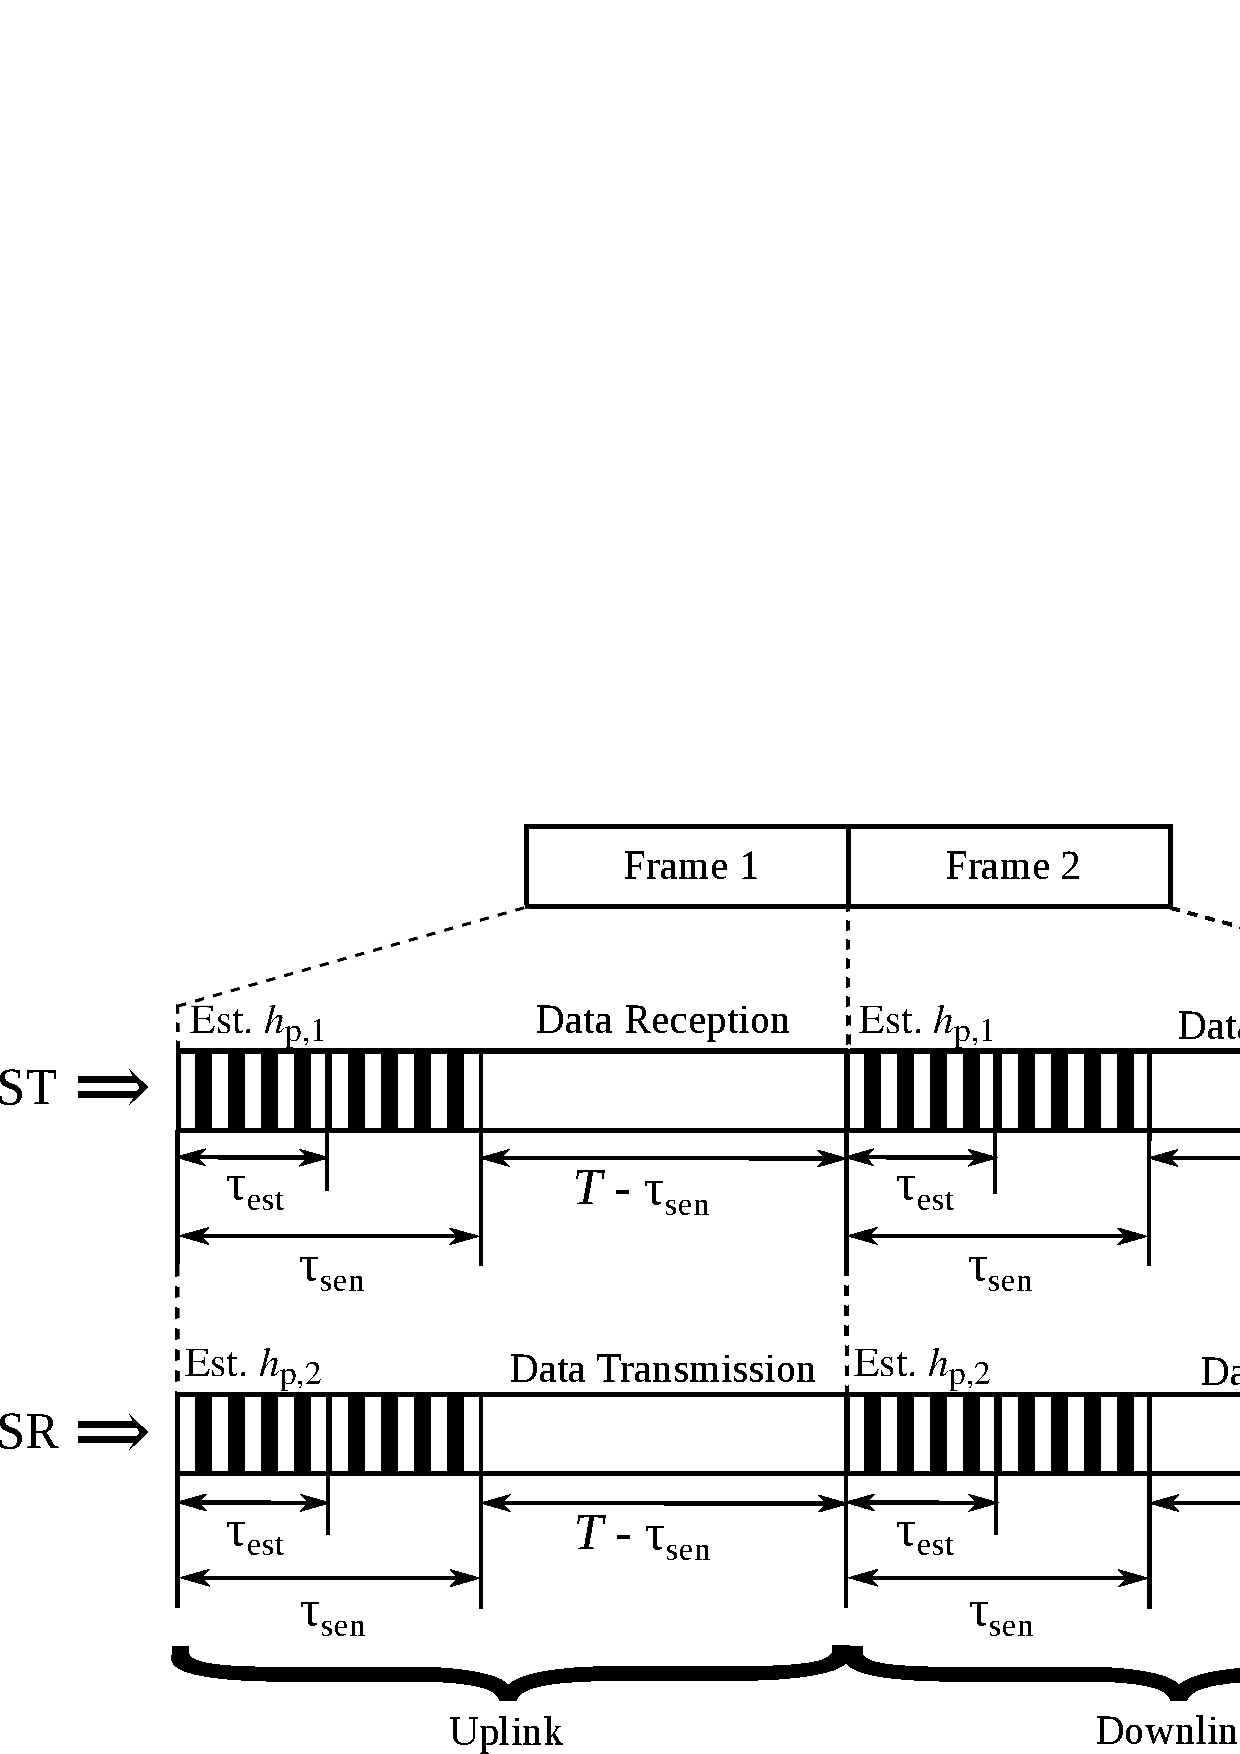
\includegraphics[width = \columnwidth]{figures/Frame_Structure}
\caption{Frame structure of the IS illustrating the time allocation of the channel estimation, sensing and data transmission from the perspective of the ST and the SR.} %The estimation of the sensing ($\hpo$) and the interference channel ($\hptw$) estimation occur at the ST. The estimation of the access channel ($\hs$) happens at the SR. Because of the employment of pilot-based channel estimation, the time resources allocated (number of sample used) for its estimation relatively less as compared to the previous two channels used for the channel estimation, it is not considered in the frame structure.} 
\label{fig_IS:fs}
%\vspace{-0.5cm}
\end{figure}
%The inclusion of estimation of the interacting channels causes variations in the parameters $\pd$, $\cz$ and $\co$. Unless characterized, these variations may seriously degrade the performance of the hardware deployed. In this view, we include the estimation of the interacting channels in the system model, thereby characterizing the variations in $\pd$, $\cz$ and $\co$ by means of their their distribution functions $\fpd$, $\fcz$ and $\fco$. By utilizing these expressions, we finally obtain a characterization of sensing-throughput tradeoff. %that depicts an deployment scenario. 
In order to include channel estimation, a frame structure that constitutes estimation $\test$, sensing $\tsen$ and data transmission $T - \tsen$ is proposed, where $\test$ and $\tsen$ correspond to time intervals and \tc{$0 < \test \le \tsen < T$, refer to} \figurename~{\ref{fig_IS:fs}}. Since the estimated values of the interacting channels are required for determining the suitable sensing time (the duration of the sensing phase), the sequence depicted in \figurename~{\ref{fig_IS:fs}} is reasonable for the hardware deployment, whereby estimation is followed by sensing.
Particularly for the sensing channel, it is worthy to note that the samples used for estimation can be combined with the samples acquired for sensing (therefore, the sensing phase incorporates the estimation phase, see \figurename~\ref{fig_IS:fs}) such that the time resources within the frame duration can be utilized efficiently, as shown in the frame structure in \figurename~\ref{fig_IS:fs}.
%To acquire the estimates for the interference and the access channels at the ST, a low-rate feedback channel from the SR to the ST is required for the proposed approach. 
Considering the fact that the number of pilot symbols is relatively small in comparison to the samples used for performing received power-based channel estimation, the time allocation of the pilot symbols does not affect the overall performance of the ISs. Hence, no time resources are allocated for the estimation of the access channel in the frame structure. In the following paragraphs, the estimation of the involved channels is considered.


\paragraph{Estimation of sensing channel ($\hpo$)}
\index{Channel estimation|(}
%To incorporate the effect of fading in the model, we assume that the channel remains constant for $T$.
\index{Channel estimation!received power-based|textbf}
Following the previous discussions, the ST acquires the knowledge of $\phpo$ (included in $\prcvdstpt$, cf. (\ref{eq_IS:pd})) to characterize $\pd$, and to further evaluate the detector's performance. This knowledge is acquired by estimating the power received at the ST over the sensing channel. %by estimating its received power. The estimated received power is required for the characterization of $\pd$, thereby evaluating the detector performance. %, an vital performance parameter for the cognitive radio system. %Implicit to estimation, the variation in the received power are translated to the $\pd$. Hence, the characterization of the $\pd$ in terms of distribution function is essential. 
%Characterized by the fading process, each frame witnesses a different received power. In order to sustain a desired detection probability, it is important to acquire the knowledge of $\prcvd$. As a result, received power estimation $\test$ precedes sensing $\tsen$ for each frame. The remaining time $T - (\test + \tsen)$ is utilized for data transmission. 

Under $\mathcal H_1$, the received power-based estimated during the estimation phase at the ST is given as \cite{Urkowitz}
\begin{align}
\eprcvdstpt = \s{\test \fsam}{ |\yrcvd[n]|^2}.
\label{eq_IS:eprcvd} 
\end{align}
$\eprcvdstpt$ determined in (\ref{eq_IS:eprcvd}) using $\test \fsam$ samples follows a \index{Distribution!central chi-squared}central chi-squared distribution $\cchi2$ \cite{Kay}. $\fsam$ and $\test$ are such that the number of samples $\test \fsam$ is an integer.
 %Applying the central limit theorem, this distribution can be approximated as the Gaussian distribution 
The cdf of $\eprcvdstpt$ is given by
\begin{align}
%\eprcvd \sim \mathcal{N}\left( \prcvd, \frac{2}{\test \fsam} \prcvd^2 \right).
%\eprcvd \sim  \cchi\left( \prcvd, \frac{2}{\test \fsam} \prcvd^2 \right).
\feprcvdstpt(x) = 1 - \Gamma\left(\frac{\test \fsam}{2}, \frac{ \test \fsam x}{2 \prcvdstpt}  \right). 
\label{eq_IS:dprcvd}
\end{align}
\paragraph{Estimation of access channel ($\hs$)}
%This information is essential for characterize the throughput $\cz$ and $\co$. 
%However, this information is not directly available at the SR.
%To accomplish this, we employ a pilot based estimation for $\hs$ and received power based estimation $\hpt$. 
%Channel estimation is a fundamental aspect to most wireless communication systems. 
The signal received from the SR undergoes matched filtering and demodulation at the ST, hence, it is reasonable to employ pilot-based estimation for $\hs$. Unlike received power-based estimation, pilot-based estimation renders a direct estimation of the channel. Now, to accomplish pilot-based estimation, the ST aligns itself to the pilot symbols transmitted by the SR.\index{Channel estimation!pilot-based|textbf}

Under $\mathcal H_0$, the discrete and complex pilot symbol at the output of the demodulator is given by \cite{Gifford08}
\begin{align}
p[n] = \sqrt{E\sub{s}} \hs + \wst[n], 
\label{eq_IS:pilot_sig}
\end{align}
where $E\sub{s}$ denotes the pilot energy. Without loss of generality, the pilot symbols are considered to be +1. The \index{Maximum likelihood estimate}maximum likelihood estimate, representing a sample average of $\Ks$ pilot symbols, is given by \cite{Gifford05}
\begin{align}
\ehs = \hs + \smash[b]{\underbrace{\frac{\sum\limits^{\Ks}_{n=1} \wst[n]}{\Ks}}_{\epsilon}},
\label{eq_IS:pilot_MLE}
\end{align}\\[-0.00em]
where $\epsilon$ denotes the estimation error.
%(\ref{eq_IS:pilot_MLE}) illustrates a correlation between the $\hs$ and $\ehs$. 
The estimate $\ehs$ is unbiased, efficient and achieves a \index{Cram\'er-Rao bound}Cram\'er-Rao bound with equality, with variance $\e{}{|\hs -\ehs|^2} = \npo/\Ks$ \cite{Gifford08}.

Consequently, $\ehs$ conditioned on $\hs$ follows a circularly symmetric Gaussian distribution.
\begin{align}
\ehs|\hs \sim \mathcal{CN}\left( \hs,\evar \right).
\label{eq_IS:ehs} 
\end{align}
As a result, the power gain $|\ehs|^2$ follows a non-central chi-squared ($\ncchi2$)\index{Distribution!non-central chi-squared} distribution with 2 degrees of freedom and non-centrality parameter $\ls = \frac{\Ks |\hs|^2}{\npo}$.

\paragraph{Estimation of interference channel ($\hpt$)}
\index{Channel estimation!received power-based}
The knowledge of $\phpt$ is required to characterize the interference from the PT.
Analog to the sensing channel, the SR performs received power-based estimation by listening to the signal transmitted by the PT.

Under $\mathcal H_1$, in the estimation phase (which implies ST is not transmitting, please consider \figurename~\ref{fig_IS:fs}), the discrete and complex signal received at the SR is given as
\begin{align}
\ys[n] = \hpt \cdot \xp[n] + \wsr[n].
\label{eq_IS:sys_mod_p2s}
\end{align}
%Under $\mathcal H_1$, the SR cancels the ST the data signal over the access channel in order to estimate the secondary interference (power) received from the PT, refer to (\ref{eq_US:sys_mod_sr}). In order to establish a preliminary analysis, it is assumed that signal to noise ratio for the access link is suitable enough to allow perfect cancellation of the data signal. For extreme situations, a probabilistic approach can be applied to deal with the imperfect signal cancellation for the proposed channel estimation. However, under such situations, it is possible that due to bad quality of the access channel, the ST may not consider such a channel for data transmission. In both situations, the received power at the SR from the PT given by  
As a result, the estimated power at the SR, from the signal transmitted by the PT, is given by
\begin{align} 
\eprcvdsr &= \frac{1}{\Kp} \sum\limits_{n = 1}^{\Kp} |\ys[n]|^2,
\label{eq_IS:ehp2}
\end{align}
where $\eprcvdsr$ follows a $\cchi2$ distribution.%, where $\Kp$ corresponds to the number of samples used for the estimation.
\index{Channel estimation|)}

\subsubsection{\tc{Validation}}
\tc{
At this stage, it is clear that the estimates $\eprcvdstpt$, $|\ehs|^2$ and $\eprcvdsr$ exhibit the knowledge corresponding to the involved channels, however, it is essential to validate them, mainly $\eprcvdstpt$ and $\eprcvdsr$. In this context, it is necessary to ensure the presence of the PU signal ($\mathcal H_1$) for that particular frame. In this direction, Chavali \textit{et al.} \cite{Chav11} recently proposed a detection followed by the estimation of the signal to noise ratio, while \cite{Cao14} implemented a blind technique for estimating the signal power of non-coherent PU signals.

Here, a different methodology is proposed, according to which a coarse detection on the estimates ($\eprcvdstpt$, $\eprcvdsr$) at the end of the estimation phase $\test$ is applied. For the coarse detection, an energy detection is employed whose threshold can be determined by means of Neyman-Pearson criterion. Through an appropriate selection of the time interval $\test$ (for instance, $\test \in [1, 10]\SI{}{ms}$) during the system design, the reliability of the coarse detection can be ensured. With the existence of a separate control channel such as cognitive pilot channel, the reliability of the coarse detection can be further enhanced by exchanging the detection results between the ST and the SR.}

\tc{
The estimation and the coarse detection processes in the proposed method are equivalent in terms of their mathematical operations, consisting of magnitude squared and summation. In this regard, the validity of the channel estimates with certain reliability and without comprising the complexity of the estimators, employed by the secondary system, is considered. Moreover, by performing a joint estimation and (coarse) detection, an efficient way of utilizing the time resources within the frame duration is proposed. The ST considers these estimates to determine a suitable sensing time based on the sensing-throughput tradeoff such that the desired detector's performance is ensured. At the end of the detection phase, a fine detection of the PU signals is carried out, thereby improving the performance of the detector. In accordance with the proposed frame structure in \figurename~\ref{fig_IS:fs}, fine detection represents the main detection, which also includes the samples acquired during the estimation phase.} 


\subsubsection{Assumptions and Approximation}
%We consider the estimation of $\bprcvd$ at the ST. To simplify the analysis for the proposed model, it is assumed that the ST acquires the perfect knowledge about $\snrp$ and $ \snrs$ from the SR over a feedback channel. 
To simplify the analysis and sustain analytical tractability for the proposed approach, several assumptions, considered in this section, are summarized as follows:
\begin{itemize}
\item All transmitted signals are subjected to distance dependent path loss and small scale fading gain. %The small scale fading gains $\gpo, \gpt, \gs$ are modelled as frequency-flat fading. %Hence, the $\gpo, \gpt, \gs$ follow a unit-mean exponential distribution \cite{Tse05}.
With no loss of generality, it is considered that the channel gains include distance dependent path loss and small scale gain. Moreover, the coherence time for the channel gain is considered to be greater than the frame duration. In scenarios, where the coherence time exceeds the frame duration, the proposed characterization depicts a lower performance bound.
\item Perfect knowledge of the noise power is assumed in the system, however, the uncertainty in noise power can be captured as a bounded interval \cite{Tan08}. Inserting this interval in the derived expressions, \tc{refer to} Sect.~\ref{sec_IS:ana}, the performance of the IS can be expressed in terms of the upper and the lower bounds.
\end{itemize}
For analytical tractability, the following approximation is considered.
\index{Approximation}
\begin{approxi} \label{ap:ap1}
\normalfont
For all degrees of freedom, $\ncchi2$ distribution can be approximated by a Gamma distribution \cite{abramo}. The parameters of the Gamma distribution are obtained by matching the first two central moments to those of $\ncchi2$.
\end{approxi}


\subsection{Theoretical Analysis} \label{sec_IS:ana}
%%%%%%%%%%%%%%%%%%%%%%%%%%%%%%%%%%%%%%%%%%%%%%%%%%%%%%%%%%%%%%%%%%%%%%%%%%%%%%%%%%%%%%%%%
%\subsection*{Characterizing the performance parameters}
%%%%%%%%%%%%%%%%%%%%%%%%%%%%%%%%%%%%%%%%%%%%%%%%%%%%%%%%%%%%%%%%%%%%%%%%%%%%%%%%%%%%%%%%%%
%The estimation of received power at the ST and interacting channels translate to the distortion in the performance parameters $\pd$ and $\trs$. 
%While substituting estimated received power $\prcvd$ in (\ref{eq_IS:pd}), a certain distortion is induced in the $\pd$. In order capture this distortion, it is essential to characterize its distribution function $\fpd$. 
\index{Channel!deterministic channel}
%\subsection{Deterministic Channel} \label{ssec_IS:det_th}
%At first, the performance of the proposed framework in context to the deterministic channel is evaluated.
At this stage, it is evident that the variation due to the imperfect channel knowledge translates to the variations in the performance parameters
\begin{align}
\epd = \Gamma\left( \frac{\tsen \fsam}{2}, \frac{\tsen \fsam \mu}{2 \eprcvdstpt} \right),  \label{eq_IS:epd} 
\end{align}
\begin{align}
\ecz = \log_2 \left(1 + \ephs \frac{\ptranst}{\npo}\right), 
\label{eq_IS:ecz} 
\end{align}
and
\begin{align}
\eco = \log_2 \left(1 + \frac{\ephs \ptranst }{\eprcvdsr} \right), 
\label{eq_IS:eco} 
\end{align}
which are fundamental to sensing-throughput tradeoff. It is worth noticing the fact (\ref{eq_IS:epd}), (\ref{eq_IS:ecz}) and (\ref{eq_IS:eco}) are determined using the estimated parameters, which include $\eprcvdstpt$, $\ephs$ and $\eprcvdsr$, determined in previous section. Below, the variations in these performance parameters are characterized in terms of their cdfs $\fpd(\cdot)$, $\fcz(\cdot)$ and $\fco(\cdot)$.
\begin{lemma} \label{lm_IS:lem1}
\normalfont
The cdf of $\epd$ is characterized as
\begin{align}
\fpd(x) = 1 - \Gamma \left(\frac{\test \fsam}{2}, \frac{\test \tsen \fsam^2 \mu}{4 \prcvdstpt \Gamma^{-1}(x, \frac{\tsen \fsam}{2}) } \right), 
%\fpd(x) = 1 - \mathcal{Q} \left( {\frac{\mu}{ \left( \sqrt{\frac{2}{\tsen \fsam}} \mathcal{Q}^{-1}(x) + 1 \right) }}\Bigg/{ \sqrt{\frac{2}{\test \fsam}} \prcvd }  \right).
%\dpd = \mu \frac{\exp \left( \frac{\left(\mathcal{Q}^{-1}(x)\right)^2}{2}  - \left( \frac{\frac{\lambda}{1 + \sqrt{\frac{2}{\tsen \fsam}} \mathcal{Q}^{-1}(x)} - \bprcvd}{ \bprcvd \sqrt{\frac{4}{\test \fsam}}}    \right)^2 \right)}{ \bprcvd \sqrt{\frac{2}{\tsen \fsam}} \left( 1 + \sqrt{\frac{2}{\test \fsam}} \mathcal{Q}^{-1}(x) \right)^2 }
\label{eq_IS:fpd}
\end{align}
where $\Gamma^{-1}(\cdot, \cdot)$ is the inverse of the regularized upper-incomplete Gamma function \cite{grad}.
\end{lemma}
\begin{proof}
The cdf of $\epd$ is defined as
\begin{align}
\fpd(x) = \p(\epd \le x).
\end{align}
Using (\ref{eq_IS:epd})
\begin{align}
\quad =  \p \left( \Gamma \left( \frac{\tsen \fsam}{2}, \frac{\tsen \fsam \mu}{2 \eprcvdstpt} \right) \le x \right), 
\end{align}
\begin{align}
\quad =  1- \p \left( \eprcvdstpt \ge \frac{\mu \tsen \fsam}{2 {\Gamma}^{-1}\left( x, \frac{\tsen \fsam}{2} \right) } \right). \label{eq_IS:lem1} 
%\quad &=  \p \left( \mathcal{Q} \left( \frac{\mu - \eprcvd}{\sqrt{\frac{2}{\tsen \fsam} }} \right) \le x \right) \\ 
%\quad &=  1- \p \left( \eprcvd \le \frac{\mu}{\mathcal{Q}^{-1}(x) \sqrt{\frac{2}{\tsen \fsam}}} \right) 
\end{align}
Replacing the cdf of $\eprcvdstpt$ in (\ref{eq_IS:lem1}), an expression of $\fpd(\cdot)$ is obtained.
\end{proof}
\begin{lemma} \label{lm_IS:lem2}
\normalfont
The cdf of $\ecz$ is defined as
\begin{align}
\fcz(x) &= \int\limits_{0}^{x} \dcz(t) dt, \label{eq_IS:dis_C0} 
\end{align}
where
\begin{align}
\dcz(x) = 2^x \ln 2 \frac{(2^x - 1)^{\as - 1}}{\Gamma(\as) \bs^{\as}} \exp\left(-\frac{2^x - 1}{\bs}\right),  \label{eq_IS:den_C0}
\end{align}
and 
\begin{align}
\as = \frac{(2 + \ls)^2}{(4 + 4\ls)} \text{ and }  \bs = \npo \frac{(4 + 4\ls)}{(2 + \ls)} \label{eq_IS:dphs_para}. 
\end{align}
%and, $\as$ and $\bs$ are defined in (\ref{eq_IS:dphs_para}).
%\begin{align}
%\quad & \as = \frac{\left(2 \lambdas + |\hs|^2  \right)^2 }{ \lambdas \left(2 \lambdas + 4 |\hs|^2  \right)}   \text{  and  } \nonumber \\ \quad & \bs = \frac{\lambdas \left(2 \lambdas + 4  |\hs|^2 \right)}{\left( \lambdas + |\hs|^2  \right) } \label{eq_IS:para_s}. 
%\end{align}
\end{lemma}
\begin{proof}
\tc{See \cite[Section IV, Lemma 2]{Kaushik16_TWC}}.
\end{proof}

\begin{lemma} \label{lm_IS:lem3}
\normalfont
The cdf of $\eco$ is given by
\begin{align}
\fco(x) = \int\limits_{0}^{x} \dco(t) dt, \label{eq_IS:dis_C1} 
\end{align}
where
\begin{align}
\dco(x) = 2^x \ln 2 \frac{(2^x - 1)^{\as - 1} \Gamma(\as + \ap)}{\Gamma(\as) \Gamma(\ap) \bs^{\as} \bp^{\ap}} \left(\frac{1}{\bp} + \frac{2^x - 1}{\bs}\right)^{(\as + \ap)}, \label{eq_IS:den_C1}
\end{align}
and
\begin{align}
\ap = \frac{\tsen \fsam}{2} \text{ and } \bp = \frac{2 \prcvdsr}{\npo \tsen\fsam}.
\end{align}
%\begin{align}
%\quad & \ap = \frac{N (1 + \snrp)^2}{(2 + 4 \snrp)} \text{  and  } \bp = \frac{\sigma^2 (2+ 4 \snrp)}{N (1 + \snrp)}, \label{eq_IS:para_p} 
%\quad & \ap = \frac{\Kp}{2}  \text{  and  } \bp = \frac{2 \prcvdsr}{\npo \Kp}, \label{eq_IS:para_p} 
%\end{align}
where $\as$ and $\bs$ are defined in (\ref{eq_IS:dphs_para}).%, whereas $\ap$ and $\bp$ are defined in (\ref{eq_IS:dsnrp_para}).
\end{lemma}
\begin{proof}
\tc{See \cite[Appendix A]{Kaushik16_TWC}}.
\end{proof}

Next, a sensing-throughput tradeoff for the estimation model is established that includes the estimation time and incorporates the variations in the performance parameter. Most importantly, to restrain the harmful effect of the uncertain interference at the PR due to the variations in the detection probability%Unless investigated, these distortions may result in harmful interference at the PR and/or reduction in the throughput at the SR. In this regard, we capture these distortions induced in the system, thereby characterizing the true performance of the IS. 
, two new PU constraints at the PR, namely an Average Constraint (AC) and an Outage Constraint (OC) on the detection probability are proposed. Based on these constraints, the sensing-throughput tradeoff for the IS is characterized.


%In order to sustain the effect of the distortion induced due to the estimation of the received power, an outage constraint on the detection probability is proposed. 
%\subsection*{Average Constraint}
%The average constraint on the detection probability is defined as
%\begin{equation}
%\e{}{\pd} \le \pdd
%\label{eq_IS:AC}
%\end{equation}
%The transformed sensing-throughput tradeoff subject to the average constraint is presented as
%\begin{figure*}
\index{Tradeoffs!estimation-sensing-throughput tradeoff}
\index{Secondary throughput}
\index{Interference constraint!average constraint}
\begin{theorem} \label{th_IS:th1}
\normalfont
The achievable expected secondary throughput subject to an average constraint on $\epd$ that employs channel estimation corresponding to the deterministic behavior of the interacting channels, is given by 
\begin{align}
\trsac(\ttest, \ttsenac) =& \maxi_{\tc{\test}, \tsen} \e{\epd, \ecz, \eco}{\rs(\test, \tsen)} \nonumber \\ 
\quad =& \frac{T- \tsen}{T} \bigg[ \e{\ecz}{\ecz} (1 - \pfa) \phz + \nonumber \\ \quad & \e{\eco}{\eco} (1 - \e{\epd}{\epd}) \pho  \bigg], \label{eq_IS:thr_AC} \\
\text{s.t.} & \text{ }  \e{\epd}{\epd} \ge \pdd, \label{eq_IS:AC} \\
\tc{\text{s.t.}} & \text{ }  \tc{0 < \test \le \tsen \le T,} \nonumber
\end{align}
\end{theorem}
% IEEE uses as a separator
%\hrulefill
% The spacer can be tweaked to stop underfull vboxes.
%\vspace*{4pt}
%\end{figure*}
%In this regard, we analyze the performance of IS based on this constraint.
where $\e{\epd}{\cdot}$ represents the expectation with respect to $\epd$, $\e{\epd, \ecz, \eco}{\cdot}$ denotes the expectation with respect to $\epd$, $\ecz$ and $\eco$. Unlike (\ref{eq_IS:thr_id_con}), $\pdd$ in (\ref{eq_IS:thr_AC}) represents the constraint on expected detection probability.

\begin{proof}
\tc{See \cite[Appendix B]{Kaushik16_TWC}.}
\end{proof}
%\subsection*{Outage Constraint}
%Here, we consider the outage constraint on the detection probability is defined as 
%\begin{equation}
%P(\pd \le \pdd) \le \mpd
%\label{eq_IS:OC}
%\end{equation}

\index{Interference constraint!outage constraint}
\begin{theorem} \label{th_IS:th2}
\normalfont
The achievable expected secondary throughput subject to an outage constraint on $\epd$ that employs channel estimation corresponding to the deterministic behavior of the interacting channels, is given by  
\begin{align}
\trsoc(\ttest, \ttsenoc) =& \maxi_{\tc{\test}, \tsen} \e{\epd, \ecz, \eco}{\rs(\test, \tsen)} \nonumber \\ 
\quad =& \frac{T- \tsen}{T} \bigg[ \e{\ecz}{\ecz} (1 - \pfa) \phz + \nonumber \\ \quad & \e{\eco}{\eco} (1 - \e{\epd}{\epd}) \pho  \bigg], \label{eq_IS:thr_OC} \\
\text{s.t.} & \text{ }  \p(\epd \le \pdd) \le \mpd, \label{eq_IS:OC} \\
\tc{\text{s.t.}} & \text{ }  \tc{0 < \test \le \tsen \le T,} \nonumber
\end{align}
\end{theorem}
%In this regard, we analyze the performance of IS based on this constraint. 
where $\mpd$ represents the outage constraint.
%\subsubsection*{Methodology of analysis}

\begin{proof}
\tc{See \cite[Appendix B]{Kaushik16_TWC}.}
\end{proof}
\tc{In contrast to the ideal model, the sensing-throughput tradeoff investigated by the estimation model (refer to Problems \ref{th_IS:th1} and \ref{th_IS:th2}) incorporates the imperfect channel knowledge. In this context, the performance characterization considered by the proposed framework is closer to the realistic situations.}
%Subsequently, following the variation of optimum expected throughput $\trs(\test,\ttsen)$ (optimized over the sensing time) against the estimation time, 
Herein, based on the estimation model, a fundamental relation between estimation time (that regulates the variation in the detection probability according to the PU constraint), sensing time (that represents the detector performance) and achievable throughput is established. This relationship is characterized as estimation-sensing-throughput tradeoff. Based on this tradeoff, a suitable estimation time $\test = \ttest$ and a suitable sensing time $\tsen = \ttsen$ that attains a maximum achievable throughput $\trs(\ttest,\ttsen)$ for the IS is determined.
%\end{remark}

\begin{corollary} \label{cor_IS:cor1}
\normalfont
\tc{Problems \ref{th_IS:th1} and \ref{th_IS:th2} consider the optimization of the expected secondary throughput to incorporate the effect of variations due to the channel estimation, and subsequently determine the suitable sensing and the suitable estimation time. Here, an alternative approach to the optimization problem that captures the effect of imperfect channel knowledge is investigated. According to which, the suitable sensing time for a certain value of estimation time, subject to the average constraint, is determined as}
\tc{
\begin{align}
\ttsen &= \argmaxi_{\tsen} \rs(\test, \tsen) \label{eq_IS:C_sen_AC} \\ 
\quad &= \frac{T- \tsen}{T} \bigg[ \ecz (1 - \pfa) \phz + \eco (1 - \epd) \pho  \bigg], \nonumber \\
\text{s.t.} & \text{ }  \e{\epd}{\epd} \ge \pdd, \nonumber \\
\tc{\text{s.t.}} & \text{ }  \tc{0 < \test \le \tsen \le T.} \nonumber
\end{align}
}
\tc{
Similarly, the suitable sensing time for a certain value of estimation time, subject to the outage constraint, is determined as}
\tc{
\begin{align}
\ttsen &= \argmaxi_{\tsen} \rs(\test, \tsen) \label{eq_IS:C_sen_OC} \\ 
\quad &= \frac{T- \tsen}{T} \bigg[ \ecz (1 - \pfa) \phz + \eco (1 - \epd) \pho  \bigg], \nonumber \\
\text{s.t.} & \text{ }   \p(\epd \le \pdd) \le \mpd, \nonumber \\
\tc{\text{s.t.}} & \text{ }  \tc{0 < \test \le \tsen \le T.} \nonumber
\end{align}
}
In contrast to (\ref{eq_IS:thr_AC}) and (\ref{eq_IS:thr_OC}), the suitable sensing time evaluated in (\ref{eq_IS:C_sen_AC}) and (\ref{eq_IS:C_sen_OC}) entails the variations due to the channel estimation from the performance parameters ($\epd, \ecz, \eco$). Hence, the expected secondary throughput subject to the average and the outage constraints that captures the variations in the suitable sensing time and the performance parameters, is determined as
\begin{align}
\e{\epd, \ecz, \eco, \ttsen}{\rs(\test, \ttsen)} \label{eq_IS:C_thr},
\end{align}
where $\e{\epd, \ecz, \eco, \ttsen}{\cdot}$ corresponds to an expectation over $\epd, \ecz, \eco, \ttsen$.

In accordance with the Problems  \ref{th_IS:th1} and \ref{th_IS:th2}, the expected secondary throughput, defined in (\ref{eq_IS:C_thr}), is further optimized over the estimation time to yield the achievable expected secondary throughput
\begin{align}
\trs(\ttest, \ttsenac) &= \maxi_{\test} \e{\epd, \ecz, \eco, \ttsen}{\rs(\test, \ttsen)} \label{eq_IS:C_thr_AC}. 
\end{align}
In this way, an estimation-sensing-throughput tradeoff for the alternative approach is established that determines the suitable estimation and the suitable sensing time intervals.
\end{corollary}
\begin{remark} \label{rm:rem2}
\normalfont
Complementing the analysis in \cite{Liang08}, it is complicated to obtain a closed-form expression of $\ttsen$, thereby rendering the analytical tractability of its cdf difficult. In this view, the performance of the alternative approach is captured by means of simulations.
\end{remark}


%%%%%%%%%%%%%%%%%%%%%%%%%%%%%%%%%%%%%%%%%%%%%%%%%%%%%%%%%%%%%%%%%%%%%%%%%%%%%%%%%%%%%%%%%
\subsection{Numerical Results} \label{sec_IS:num_ana}
%%%%%%%%%%%%%%%%%%%%%%%%%%%%%%%%%%%%%%%%%%%%%%%%%%%%%%%%%%%%%%%%%%%%%%%%%%%%%%%%%%%%%%%%%
Here, the performance of the IS based on the proposed approach is investigated. In this regard: (i) the simulations are performed to validate the expressions obtained, (ii) the performance degradation incurred due to the channel estimation is analyzed. In this regard, the ideal model is considered to benchmark, and to evaluate the performance loss, (iii) the mathematical justification to the considered approximations is established. Although the derived expressions, depicting the performance analysis, are general and applicable to all CR systems, the parameters are selected in such a way that they closely relate to the deployment scenario described in \figurename~{\ref{fig_IS:scenario}. Unless stated explicitly, the choice of the parameters given in Table \ref{tb_IS:tb2} is considered for the analysis.
\begin{table}
%\vspace{-0.4cm}
\renewcommand{\arraystretch}{1.4}
\caption{Parameters for Numerical Analysis}
%\vspace{-0.6cm}
\label{tb_IS:tb2}
\centering
%\small{
\begin{tabular}{c||c}
\hline
\bfseries Parameter & \bfseries Value \\
\hline\hline
$\fsam$  & $\SI{1}{MHz}$ \\ %\hline
$\phpo$  & $\SI{-100}{dB}$ \\ %\hline
$\phpt$  & $\SI{-100}{dB}$ \\ %\hline
$\phs$  & $\SI{-80}{dB}$ \\ %\hline 
$T$ & $\SI{100}{ms}$ \\ %\hline 
$\pdd$ & 0.9 \\ %\hline 
$\mpd$ & $0.05$ \\ %\hline 
$\npo$ & $\SI{-100}{dBm}$ \\ %\hline
$\snrrcvd$ & $\SI{-10}{dB}$ \\ %\hline
$\snrpt$ & $\SI{-10}{dB}$ \\ %\hline
$\snrso$ & $\SI{10}{dB}$ \\ %\hline
$\spo = \ptranpt$ & $-\SI{10}{dBm}$ \\ %\hline
$\ptranst$ & $-\SI{10}{dBm}$ \\ %\hline
$\pho = 1 - \phz$ & 0.2 \\ %\hline
$\test$ & $\SI{5}{ms}$ \\ %\hline
$\Ks$ & 10 \\ \hline
%$\Kp$ & $1000$ \\ \hline
\end{tabular}
%}
\end{table}

\begin{figure}[!ht]
\centering
\resizebox{\resizescale}{!}{%
%% Add psfrag entries
% This file is generated by the MATLAB m-file laprint.m. It can be included
% into LaTeX documents using the packages graphicx, color and psfrag.
% It is accompanied by a postscript file. A sample LaTeX file is:
%    \documentclass{article}\usepackage{graphicx,color,psfrag}
%    \begin{document}% This file is generated by the MATLAB m-file laprint.m. It can be included
% into LaTeX documents using the packages graphicx, color and psfrag.
% It is accompanied by a postscript file. A sample LaTeX file is:
%    \documentclass{article}\usepackage{graphicx,color,psfrag}
%    \begin{document}% This file is generated by the MATLAB m-file laprint.m. It can be included
% into LaTeX documents using the packages graphicx, color and psfrag.
% It is accompanied by a postscript file. A sample LaTeX file is:
%    \documentclass{article}\usepackage{graphicx,color,psfrag}
%    \begin{document}\input{fig_thr_sen_time_tradeoff_AWGN}\end{document}
% See http://www.mathworks.de/matlabcentral/fileexchange/loadFile.do?objectId=4638
% for recent versions of laprint.m.
%
% created by:           LaPrint version 3.16 (13.9.2004)
% created on:           18-Aug-2016 10:50:24
% eps bounding box:     16 cm x 12 cm
% comment:              
%
%\begin{psfrags}%
%\psfragscanon%
%
% text strings:
\psfrag{s08}[b][b]{\fontsize{8}{12}\fontseries{m}\mathversion{normal}\fontshape{n}\selectfont \color[rgb]{0,0,0}\setlength{\tabcolsep}{0pt}\begin{tabular}{c}$\rs(\test = \SI{5}{ms}, \tsen)$ [bits/sec/Hz]\end{tabular}}%
\psfrag{s09}[t][t]{\fontsize{8}{12}\fontseries{m}\mathversion{normal}\fontshape{n}\selectfont \color[rgb]{0,0,0}\setlength{\tabcolsep}{0pt}\begin{tabular}{c}$\tsen$ [ms]\end{tabular}}%
\psfrag{s13}[][]{\fontsize{10}{15}\fontseries{m}\mathversion{normal}\fontshape{n}\selectfont \color[rgb]{0,0,0}\setlength{\tabcolsep}{0pt}\begin{tabular}{c} \end{tabular}}%
\psfrag{s14}[][]{\fontsize{10}{15}\fontseries{m}\mathversion{normal}\fontshape{n}\selectfont \color[rgb]{0,0,0}\setlength{\tabcolsep}{0pt}\begin{tabular}{c} \end{tabular}}%
\psfrag{s15}[l][l]{\fontsize{8}{12}\fontseries{m}\mathversion{normal}\fontshape{n}\selectfont \color[rgb]{0,0,0}Simulated}%
\psfrag{s16}[l][l]{\fontsize{8}{12}\fontseries{m}\mathversion{normal}\fontshape{n}\selectfont \color[rgb]{0,0,0}IM}%
\psfrag{s17}[l][l]{\fontsize{8}{12}\fontseries{m}\mathversion{normal}\fontshape{n}\selectfont \color[rgb]{0,0,0}EM-AC, Problem 1}%
\psfrag{s18}[l][l]{\fontsize{8}{12}\fontseries{m}\mathversion{normal}\fontshape{n}\selectfont \color[rgb]{0,0,0}EM-OC, Problem 2}%
\psfrag{s19}[l][l]{\fontsize{8}{12}\fontseries{m}\mathversion{normal}\fontshape{n}\selectfont \color[rgb]{0,0,0}$\trs(\test,\ttsen)$}%
\psfrag{s20}[l][l]{\fontsize{8}{12}\fontseries{m}\mathversion{normal}\fontshape{n}\selectfont \color[rgb]{0,0,0}Simulated}%
\psfrag{s21}[b][b]{\fontsize{8}{12}\fontseries{m}\mathversion{normal}\fontshape{n}\selectfont \color[rgb]{0,0,0}\setlength{\tabcolsep}{0pt}\begin{tabular}{c}Zoom\end{tabular}}%
%
% axes font properties:
\fontsize{8}{12}\fontseries{m}\mathversion{normal}%
\fontshape{n}\selectfont%
%
% xticklabels:
\psfrag{x01}[t][t]{5}%
\psfrag{x02}[t][t]{5.2}%
\psfrag{x03}[t][t]{5.4}%
\psfrag{x04}[t][t]{5.6}%
\psfrag{x05}[t][t]{1}%
\psfrag{x06}[t][t]{2}%
\psfrag{x07}[t][t]{3}%
\psfrag{x08}[t][t]{4}%
\psfrag{x09}[t][t]{5}%
\psfrag{x10}[t][t]{6}%
\psfrag{x11}[t][t]{7}%
\psfrag{x12}[t][t]{8}%
\psfrag{x13}[t][t]{9}%
\psfrag{x14}[t][t]{10}%
%
% yticklabels:
\psfrag{v01}[r][r]{2.55}%
\psfrag{v02}[r][r]{2.6}%
\psfrag{v03}[r][r]{2.65}%
\psfrag{v04}[r][r]{0}%
\psfrag{v05}[r][r]{0.5}%
\psfrag{v06}[r][r]{1}%
\psfrag{v07}[r][r]{1.5}%
\psfrag{v08}[r][r]{2}%
\psfrag{v09}[r][r]{2.5}%
%
% Figure:
%\resizebox{8cm}{!}{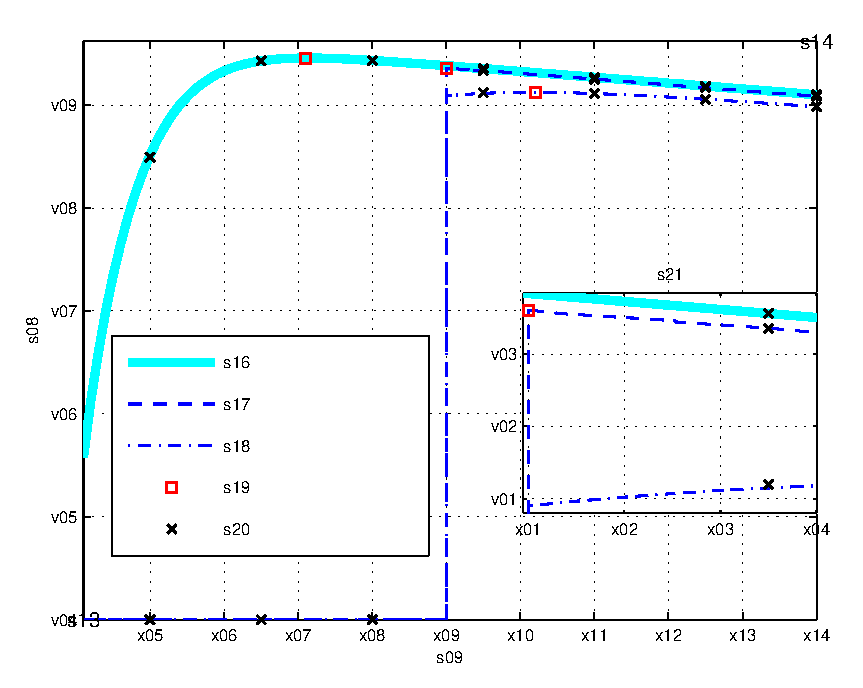
\includegraphics{fig_thr_sen_time_tradeoff_AWGN.eps}}%
%\end{psfrags}%
%
% End fig_thr_sen_time_tradeoff_AWGN.tex
\end{document}
% See http://www.mathworks.de/matlabcentral/fileexchange/loadFile.do?objectId=4638
% for recent versions of laprint.m.
%
% created by:           LaPrint version 3.16 (13.9.2004)
% created on:           18-Aug-2016 10:50:24
% eps bounding box:     16 cm x 12 cm
% comment:              
%
%\begin{psfrags}%
%\psfragscanon%
%
% text strings:
\psfrag{s08}[b][b]{\fontsize{8}{12}\fontseries{m}\mathversion{normal}\fontshape{n}\selectfont \color[rgb]{0,0,0}\setlength{\tabcolsep}{0pt}\begin{tabular}{c}$\rs(\test = \SI{5}{ms}, \tsen)$ [bits/sec/Hz]\end{tabular}}%
\psfrag{s09}[t][t]{\fontsize{8}{12}\fontseries{m}\mathversion{normal}\fontshape{n}\selectfont \color[rgb]{0,0,0}\setlength{\tabcolsep}{0pt}\begin{tabular}{c}$\tsen$ [ms]\end{tabular}}%
\psfrag{s13}[][]{\fontsize{10}{15}\fontseries{m}\mathversion{normal}\fontshape{n}\selectfont \color[rgb]{0,0,0}\setlength{\tabcolsep}{0pt}\begin{tabular}{c} \end{tabular}}%
\psfrag{s14}[][]{\fontsize{10}{15}\fontseries{m}\mathversion{normal}\fontshape{n}\selectfont \color[rgb]{0,0,0}\setlength{\tabcolsep}{0pt}\begin{tabular}{c} \end{tabular}}%
\psfrag{s15}[l][l]{\fontsize{8}{12}\fontseries{m}\mathversion{normal}\fontshape{n}\selectfont \color[rgb]{0,0,0}Simulated}%
\psfrag{s16}[l][l]{\fontsize{8}{12}\fontseries{m}\mathversion{normal}\fontshape{n}\selectfont \color[rgb]{0,0,0}IM}%
\psfrag{s17}[l][l]{\fontsize{8}{12}\fontseries{m}\mathversion{normal}\fontshape{n}\selectfont \color[rgb]{0,0,0}EM-AC, Problem 1}%
\psfrag{s18}[l][l]{\fontsize{8}{12}\fontseries{m}\mathversion{normal}\fontshape{n}\selectfont \color[rgb]{0,0,0}EM-OC, Problem 2}%
\psfrag{s19}[l][l]{\fontsize{8}{12}\fontseries{m}\mathversion{normal}\fontshape{n}\selectfont \color[rgb]{0,0,0}$\trs(\test,\ttsen)$}%
\psfrag{s20}[l][l]{\fontsize{8}{12}\fontseries{m}\mathversion{normal}\fontshape{n}\selectfont \color[rgb]{0,0,0}Simulated}%
\psfrag{s21}[b][b]{\fontsize{8}{12}\fontseries{m}\mathversion{normal}\fontshape{n}\selectfont \color[rgb]{0,0,0}\setlength{\tabcolsep}{0pt}\begin{tabular}{c}Zoom\end{tabular}}%
%
% axes font properties:
\fontsize{8}{12}\fontseries{m}\mathversion{normal}%
\fontshape{n}\selectfont%
%
% xticklabels:
\psfrag{x01}[t][t]{5}%
\psfrag{x02}[t][t]{5.2}%
\psfrag{x03}[t][t]{5.4}%
\psfrag{x04}[t][t]{5.6}%
\psfrag{x05}[t][t]{1}%
\psfrag{x06}[t][t]{2}%
\psfrag{x07}[t][t]{3}%
\psfrag{x08}[t][t]{4}%
\psfrag{x09}[t][t]{5}%
\psfrag{x10}[t][t]{6}%
\psfrag{x11}[t][t]{7}%
\psfrag{x12}[t][t]{8}%
\psfrag{x13}[t][t]{9}%
\psfrag{x14}[t][t]{10}%
%
% yticklabels:
\psfrag{v01}[r][r]{2.55}%
\psfrag{v02}[r][r]{2.6}%
\psfrag{v03}[r][r]{2.65}%
\psfrag{v04}[r][r]{0}%
\psfrag{v05}[r][r]{0.5}%
\psfrag{v06}[r][r]{1}%
\psfrag{v07}[r][r]{1.5}%
\psfrag{v08}[r][r]{2}%
\psfrag{v09}[r][r]{2.5}%
%
% Figure:
%\resizebox{8cm}{!}{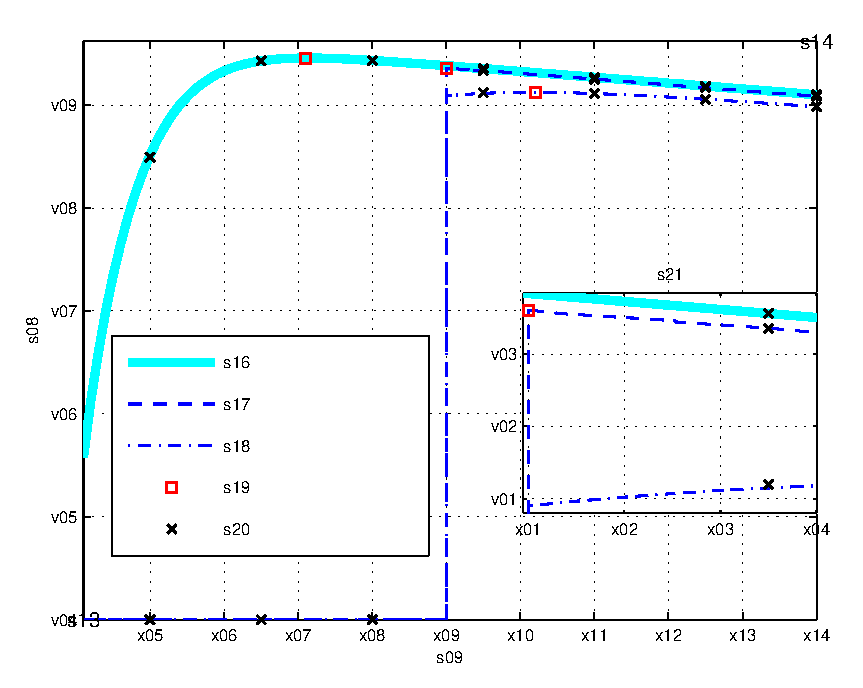
\includegraphics{fig_thr_sen_time_tradeoff_AWGN.eps}}%
%\end{psfrags}%
%
% End fig_thr_sen_time_tradeoff_AWGN.tex
\end{document}
% See http://www.mathworks.de/matlabcentral/fileexchange/loadFile.do?objectId=4638
% for recent versions of laprint.m.
%
% created by:           LaPrint version 3.16 (13.9.2004)
% created on:           18-Aug-2016 10:50:24
% eps bounding box:     16 cm x 12 cm
% comment:              
%
%\begin{psfrags}%
%\psfragscanon%
%
% text strings:
\psfrag{s08}[b][b]{\fontsize{8}{12}\fontseries{m}\mathversion{normal}\fontshape{n}\selectfont \color[rgb]{0,0,0}\setlength{\tabcolsep}{0pt}\begin{tabular}{c}$\rs(\test = \SI{5}{ms}, \tsen)$ [bits/sec/Hz]\end{tabular}}%
\psfrag{s09}[t][t]{\fontsize{8}{12}\fontseries{m}\mathversion{normal}\fontshape{n}\selectfont \color[rgb]{0,0,0}\setlength{\tabcolsep}{0pt}\begin{tabular}{c}$\tsen$ [ms]\end{tabular}}%
\psfrag{s13}[][]{\fontsize{10}{15}\fontseries{m}\mathversion{normal}\fontshape{n}\selectfont \color[rgb]{0,0,0}\setlength{\tabcolsep}{0pt}\begin{tabular}{c} \end{tabular}}%
\psfrag{s14}[][]{\fontsize{10}{15}\fontseries{m}\mathversion{normal}\fontshape{n}\selectfont \color[rgb]{0,0,0}\setlength{\tabcolsep}{0pt}\begin{tabular}{c} \end{tabular}}%
\psfrag{s15}[l][l]{\fontsize{8}{12}\fontseries{m}\mathversion{normal}\fontshape{n}\selectfont \color[rgb]{0,0,0}Simulated}%
\psfrag{s16}[l][l]{\fontsize{8}{12}\fontseries{m}\mathversion{normal}\fontshape{n}\selectfont \color[rgb]{0,0,0}IM}%
\psfrag{s17}[l][l]{\fontsize{8}{12}\fontseries{m}\mathversion{normal}\fontshape{n}\selectfont \color[rgb]{0,0,0}EM-AC, Problem 1}%
\psfrag{s18}[l][l]{\fontsize{8}{12}\fontseries{m}\mathversion{normal}\fontshape{n}\selectfont \color[rgb]{0,0,0}EM-OC, Problem 2}%
\psfrag{s19}[l][l]{\fontsize{8}{12}\fontseries{m}\mathversion{normal}\fontshape{n}\selectfont \color[rgb]{0,0,0}$\trs(\test,\ttsen)$}%
\psfrag{s20}[l][l]{\fontsize{8}{12}\fontseries{m}\mathversion{normal}\fontshape{n}\selectfont \color[rgb]{0,0,0}Simulated}%
\psfrag{s21}[b][b]{\fontsize{8}{12}\fontseries{m}\mathversion{normal}\fontshape{n}\selectfont \color[rgb]{0,0,0}\setlength{\tabcolsep}{0pt}\begin{tabular}{c}Zoom\end{tabular}}%
%
% axes font properties:
\fontsize{8}{12}\fontseries{m}\mathversion{normal}%
\fontshape{n}\selectfont%
%
% xticklabels:
\psfrag{x01}[t][t]{5}%
\psfrag{x02}[t][t]{5.2}%
\psfrag{x03}[t][t]{5.4}%
\psfrag{x04}[t][t]{5.6}%
\psfrag{x05}[t][t]{1}%
\psfrag{x06}[t][t]{2}%
\psfrag{x07}[t][t]{3}%
\psfrag{x08}[t][t]{4}%
\psfrag{x09}[t][t]{5}%
\psfrag{x10}[t][t]{6}%
\psfrag{x11}[t][t]{7}%
\psfrag{x12}[t][t]{8}%
\psfrag{x13}[t][t]{9}%
\psfrag{x14}[t][t]{10}%
%
% yticklabels:
\psfrag{v01}[r][r]{2.55}%
\psfrag{v02}[r][r]{2.6}%
\psfrag{v03}[r][r]{2.65}%
\psfrag{v04}[r][r]{0}%
\psfrag{v05}[r][r]{0.5}%
\psfrag{v06}[r][r]{1}%
\psfrag{v07}[r][r]{1.5}%
\psfrag{v08}[r][r]{2}%
\psfrag{v09}[r][r]{2.5}%
%
% Figure:
%\resizebox{8cm}{!}{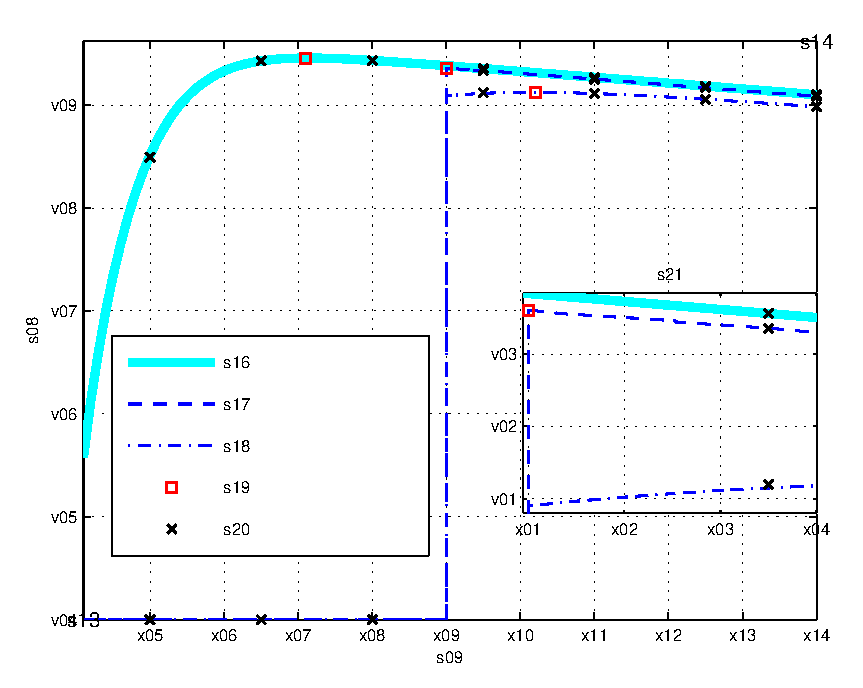
\includegraphics{fig_thr_sen_time_tradeoff_AWGN.eps}}%
%\end{psfrags}%
%
% End fig_thr_sen_time_tradeoff_AWGN.tex


\begin{tikzpicture}[scale=1]
\node[anchor=south west,inner sep=0] (image) at (0,0)
{
        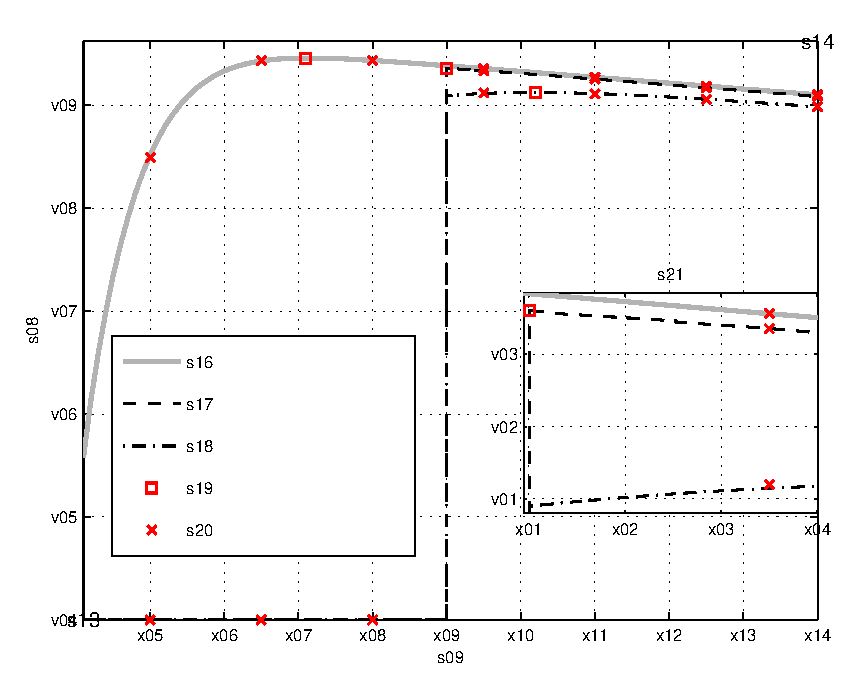
\includegraphics[width= \figscale]{figures/fig_thr_sen_time_tradeoff_AWGN}
};
\begin{scope}[x={(image.south east)},y={(image.north west)}]

%\node[draw,fill=gray!10,font=\small] (senid) at (0.232,0.83) {$\trs$};
%\draw[black, ->] (senid.north) -- (0.232,0.93);
%\node[draw,fill=gray!10,font=\small] (senac) at (0.378,0.882) {$\trsac$};
%\draw[black, ->] (senac.east) -- (0.478,0.882);
%\node[draw,fill=gray!10,font=\small] (senoc) at (0.614,0.733) {$\trsoc$};
%\draw[black, ->] (senoc.north) -- (0.614,0.833);

\draw[black,thick,<->] (0.088,0.1) --  node[above, font=\footnotesize] {$\test$} (0.512,0.1);

%\draw[help lines,xstep=.1,ystep=.1] (0,0) grid (1,1);
%\foreach \x in {0,1,...,9} { \node [anchor=north] at (\x/10,0) {0.\x}; }
%\foreach \y in {0,1,...,9} { \node [anchor=east] at (0,\y/10) {0.\y}; }
\end{scope}
\end{tikzpicture}
}
\caption{\tc{Sensing-throughput tradeoff for the Ideal Model (IM) and Estimation Model (EM), $\snrrcvd = \SI{-10}{dB}$, $\test = \SI{5}{ms}$ and $\mpd = 0.05$.}}
\label{fig_IS:ST_gen}
\vspace{-0.0cm}
\end{figure}

At first, the performance of the IS in terms of sensing-throughput tradeoff corresponding to the Ideal Model (IM) and Estimation Model (EM) for a fixed $\test = \SI{5}{ms}$ is analyzed, \tc{refer to} \figurename~\ref{fig_IS:ST_gen}. In contrast to constraint on $\pd$ for the ideal model, the average constraint (EM-AC) and the outage constraint (EM-OC) for the proposed estimation model are employed. With the inclusion of received power-based estimation in the frame structure, the ST achieves no throughput at the SR for the interval $\test$. For the given cases, namely, IM, EM-AC and EM-OC, a suitable sensing time that results in a maximum secondary throughput $\trs(\test = \SI{5}{ms},\ttsen)$ is determined. Apart from that, a performance degradation is depicted in terms of the achievable throughput, refer to \figurename~\ref{fig_IS:ST_gen}. For $\mpd = 0.05$, it is observed that the outage constraint is more sensitive to the performance loss in comparison to the average constraint. It is clear that the analysis, illustrated in \figurename~\ref{fig_IS:ST_gen}, is obtained for a certain choice of system parameters, particularly $\snrrcvd = -\SI{10}{dB}$, $\test = \SI{5}{ms}$ and $\mpd = 0.05$. To acquire more insights, the effect of these variations on the performance parameters is considered, subsequently.


\begin{figure}[!ht]

\centering
\resizebox{\resizescale}{!}{%
%% Add psfrag entries
% This file is generated by the MATLAB m-file laprint.m. It can be included
% into LaTeX documents using the packages graphicx, color and psfrag.
% It is accompanied by a postscript file. A sample LaTeX file is:
%    \documentclass{article}\usepackage{graphicx,color,psfrag}
%    \begin{document}% This file is generated by the MATLAB m-file laprint.m. It can be included
% into LaTeX documents using the packages graphicx, color and psfrag.
% It is accompanied by a postscript file. A sample LaTeX file is:
%    \documentclass{article}\usepackage{graphicx,color,psfrag}
%    \begin{document}% This file is generated by the MATLAB m-file laprint.m. It can be included
% into LaTeX documents using the packages graphicx, color and psfrag.
% It is accompanied by a postscript file. A sample LaTeX file is:
%    \documentclass{article}\usepackage{graphicx,color,psfrag}
%    \begin{document}\input{fig_opt_thr_vs_SNR_AWGN}\end{document}
% See http://www.mathworks.de/matlabcentral/fileexchange/loadFile.do?objectId=4638
% for recent versions of laprint.m.
%
% created by:           LaPrint version 3.16 (13.9.2004)
% created on:           21-Feb-2016 20:15:31
% eps bounding box:     12 cm x 9 cm
% comment:              
%
%\begin{psfrags}%
%\psfragscanon%
%
% text strings:
\psfrag{s05}[b][b]{\fontsize{8}{12}\fontseries{m}\mathversion{normal}\fontshape{n}\selectfont \color[rgb]{0,0,0}\setlength{\tabcolsep}{0pt}\begin{tabular}{c}$\rs(\testpt, \testptsr, \testpr, \ttsen)$ [bits/sec/Hz]\end{tabular}}%
\psfrag{s06}[t][t]{\fontsize{8}{12}\fontseries{m}\mathversion{normal}\fontshape{n}\selectfont \color[rgb]{0,0,0}\setlength{\tabcolsep}{0pt}\begin{tabular}{c}$\phpth$ [dB]\end{tabular}}%
\psfrag{s10}[][]{\fontsize{10}{15}\fontseries{m}\mathversion{normal}\fontshape{n}\selectfont \color[rgb]{0,0,0}\setlength{\tabcolsep}{0pt}\begin{tabular}{c} \end{tabular}}%
\psfrag{s11}[][]{\fontsize{10}{15}\fontseries{m}\mathversion{normal}\fontshape{n}\selectfont \color[rgb]{0,0,0}\setlength{\tabcolsep}{0pt}\begin{tabular}{c} \end{tabular}}%
\psfrag{s12}[l][l]{\fontsize{8}{12}\fontseries{m}\mathversion{normal}\fontshape{n}\selectfont \color[rgb]{0,0,0}EM}%
\psfrag{s13}[l][l]{\fontsize{8}{12}\fontseries{m}\mathversion{normal}\fontshape{n}\selectfont \color[rgb]{0,0,0}IM}%
\psfrag{s14}[l][l]{\fontsize{8}{12}\fontseries{m}\mathversion{normal}\fontshape{n}\selectfont \color[rgb]{0,0,0}EM}%
%
% axes font properties:
\fontsize{8}{12}\fontseries{m}\mathversion{normal}%
\fontshape{n}\selectfont%
%
% xticklabels:
\psfrag{x01}[t][t]{-110}%
\psfrag{x02}[t][t]{-105}%
\psfrag{x03}[t][t]{-100}%
\psfrag{x04}[t][t]{-95}%
\psfrag{x05}[t][t]{-90}%
%
% yticklabels:
\psfrag{v01}[r][r]{1.8}%
\psfrag{v02}[r][r]{2}%
\psfrag{v03}[r][r]{2.2}%
\psfrag{v04}[r][r]{2.4}%
\psfrag{v05}[r][r]{2.6}%
\psfrag{v06}[r][r]{2.8}%
\psfrag{v07}[r][r]{3}%
\psfrag{v08}[r][r]{3.2}%
\psfrag{v09}[r][r]{3.4}%
%
% Figure:
%\resizebox{6cm}{!}{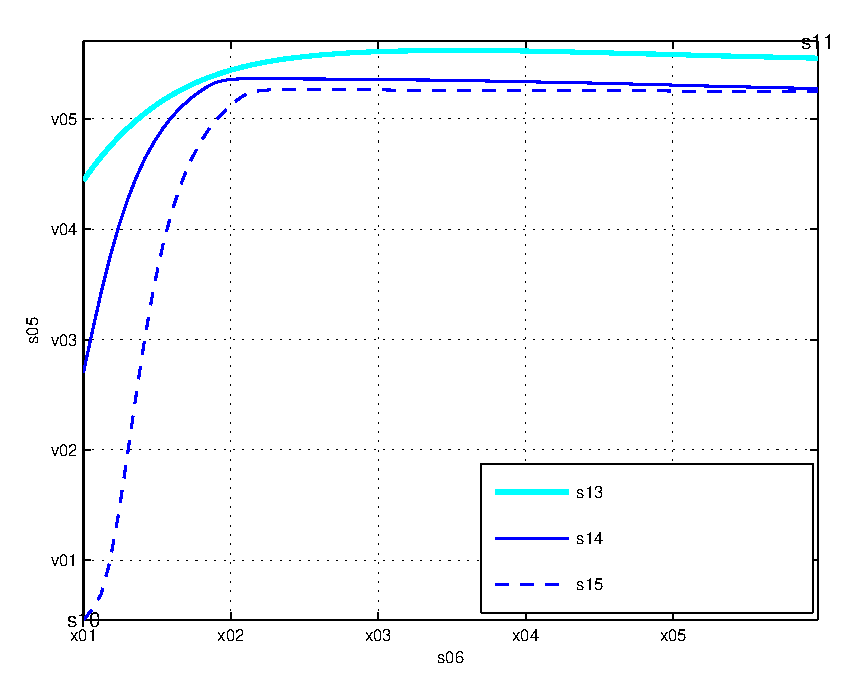
\includegraphics{fig_opt_thr_vs_SNR_AWGN.eps}}%
%\end{psfrags}%
%
% End fig_opt_thr_vs_SNR_AWGN.tex
\end{document}
% See http://www.mathworks.de/matlabcentral/fileexchange/loadFile.do?objectId=4638
% for recent versions of laprint.m.
%
% created by:           LaPrint version 3.16 (13.9.2004)
% created on:           21-Feb-2016 20:15:31
% eps bounding box:     12 cm x 9 cm
% comment:              
%
%\begin{psfrags}%
%\psfragscanon%
%
% text strings:
\psfrag{s05}[b][b]{\fontsize{8}{12}\fontseries{m}\mathversion{normal}\fontshape{n}\selectfont \color[rgb]{0,0,0}\setlength{\tabcolsep}{0pt}\begin{tabular}{c}$\rs(\testpt, \testptsr, \testpr, \ttsen)$ [bits/sec/Hz]\end{tabular}}%
\psfrag{s06}[t][t]{\fontsize{8}{12}\fontseries{m}\mathversion{normal}\fontshape{n}\selectfont \color[rgb]{0,0,0}\setlength{\tabcolsep}{0pt}\begin{tabular}{c}$\phpth$ [dB]\end{tabular}}%
\psfrag{s10}[][]{\fontsize{10}{15}\fontseries{m}\mathversion{normal}\fontshape{n}\selectfont \color[rgb]{0,0,0}\setlength{\tabcolsep}{0pt}\begin{tabular}{c} \end{tabular}}%
\psfrag{s11}[][]{\fontsize{10}{15}\fontseries{m}\mathversion{normal}\fontshape{n}\selectfont \color[rgb]{0,0,0}\setlength{\tabcolsep}{0pt}\begin{tabular}{c} \end{tabular}}%
\psfrag{s12}[l][l]{\fontsize{8}{12}\fontseries{m}\mathversion{normal}\fontshape{n}\selectfont \color[rgb]{0,0,0}EM}%
\psfrag{s13}[l][l]{\fontsize{8}{12}\fontseries{m}\mathversion{normal}\fontshape{n}\selectfont \color[rgb]{0,0,0}IM}%
\psfrag{s14}[l][l]{\fontsize{8}{12}\fontseries{m}\mathversion{normal}\fontshape{n}\selectfont \color[rgb]{0,0,0}EM}%
%
% axes font properties:
\fontsize{8}{12}\fontseries{m}\mathversion{normal}%
\fontshape{n}\selectfont%
%
% xticklabels:
\psfrag{x01}[t][t]{-110}%
\psfrag{x02}[t][t]{-105}%
\psfrag{x03}[t][t]{-100}%
\psfrag{x04}[t][t]{-95}%
\psfrag{x05}[t][t]{-90}%
%
% yticklabels:
\psfrag{v01}[r][r]{1.8}%
\psfrag{v02}[r][r]{2}%
\psfrag{v03}[r][r]{2.2}%
\psfrag{v04}[r][r]{2.4}%
\psfrag{v05}[r][r]{2.6}%
\psfrag{v06}[r][r]{2.8}%
\psfrag{v07}[r][r]{3}%
\psfrag{v08}[r][r]{3.2}%
\psfrag{v09}[r][r]{3.4}%
%
% Figure:
%\resizebox{6cm}{!}{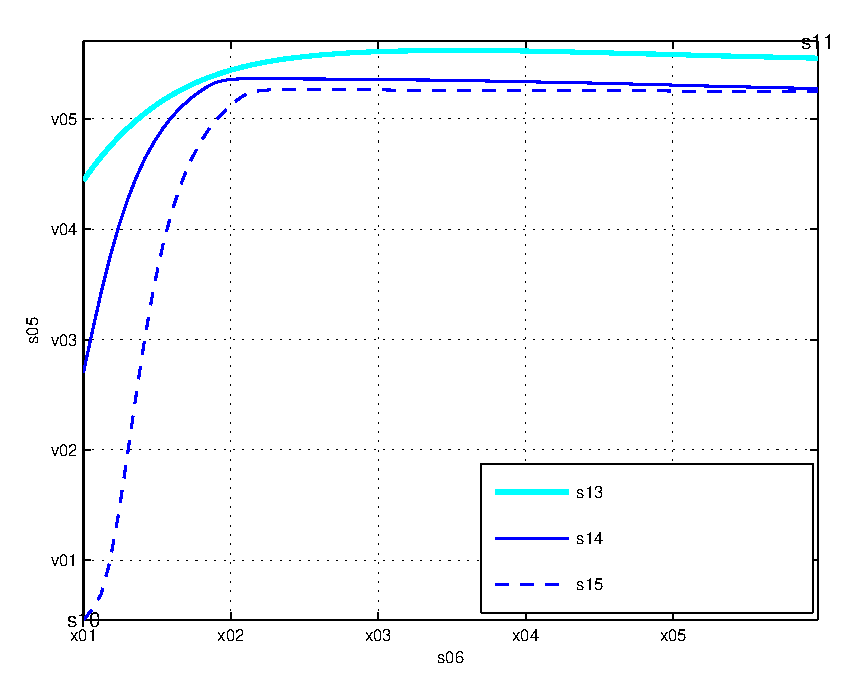
\includegraphics{fig_opt_thr_vs_SNR_AWGN.eps}}%
%\end{psfrags}%
%
% End fig_opt_thr_vs_SNR_AWGN.tex
\end{document}
% See http://www.mathworks.de/matlabcentral/fileexchange/loadFile.do?objectId=4638
% for recent versions of laprint.m.
%
% created by:           LaPrint version 3.16 (13.9.2004)
% created on:           21-Feb-2016 20:15:31
% eps bounding box:     12 cm x 9 cm
% comment:              
%
%\begin{psfrags}%
%\psfragscanon%
%
% text strings:
\psfrag{s05}[b][b]{\fontsize{8}{12}\fontseries{m}\mathversion{normal}\fontshape{n}\selectfont \color[rgb]{0,0,0}\setlength{\tabcolsep}{0pt}\begin{tabular}{c}$\rs(\testpt, \testptsr, \testpr, \ttsen)$ [bits/sec/Hz]\end{tabular}}%
\psfrag{s06}[t][t]{\fontsize{8}{12}\fontseries{m}\mathversion{normal}\fontshape{n}\selectfont \color[rgb]{0,0,0}\setlength{\tabcolsep}{0pt}\begin{tabular}{c}$\phpth$ [dB]\end{tabular}}%
\psfrag{s10}[][]{\fontsize{10}{15}\fontseries{m}\mathversion{normal}\fontshape{n}\selectfont \color[rgb]{0,0,0}\setlength{\tabcolsep}{0pt}\begin{tabular}{c} \end{tabular}}%
\psfrag{s11}[][]{\fontsize{10}{15}\fontseries{m}\mathversion{normal}\fontshape{n}\selectfont \color[rgb]{0,0,0}\setlength{\tabcolsep}{0pt}\begin{tabular}{c} \end{tabular}}%
\psfrag{s12}[l][l]{\fontsize{8}{12}\fontseries{m}\mathversion{normal}\fontshape{n}\selectfont \color[rgb]{0,0,0}EM}%
\psfrag{s13}[l][l]{\fontsize{8}{12}\fontseries{m}\mathversion{normal}\fontshape{n}\selectfont \color[rgb]{0,0,0}IM}%
\psfrag{s14}[l][l]{\fontsize{8}{12}\fontseries{m}\mathversion{normal}\fontshape{n}\selectfont \color[rgb]{0,0,0}EM}%
%
% axes font properties:
\fontsize{8}{12}\fontseries{m}\mathversion{normal}%
\fontshape{n}\selectfont%
%
% xticklabels:
\psfrag{x01}[t][t]{-110}%
\psfrag{x02}[t][t]{-105}%
\psfrag{x03}[t][t]{-100}%
\psfrag{x04}[t][t]{-95}%
\psfrag{x05}[t][t]{-90}%
%
% yticklabels:
\psfrag{v01}[r][r]{1.8}%
\psfrag{v02}[r][r]{2}%
\psfrag{v03}[r][r]{2.2}%
\psfrag{v04}[r][r]{2.4}%
\psfrag{v05}[r][r]{2.6}%
\psfrag{v06}[r][r]{2.8}%
\psfrag{v07}[r][r]{3}%
\psfrag{v08}[r][r]{3.2}%
\psfrag{v09}[r][r]{3.4}%
%
% Figure:
%\resizebox{6cm}{!}{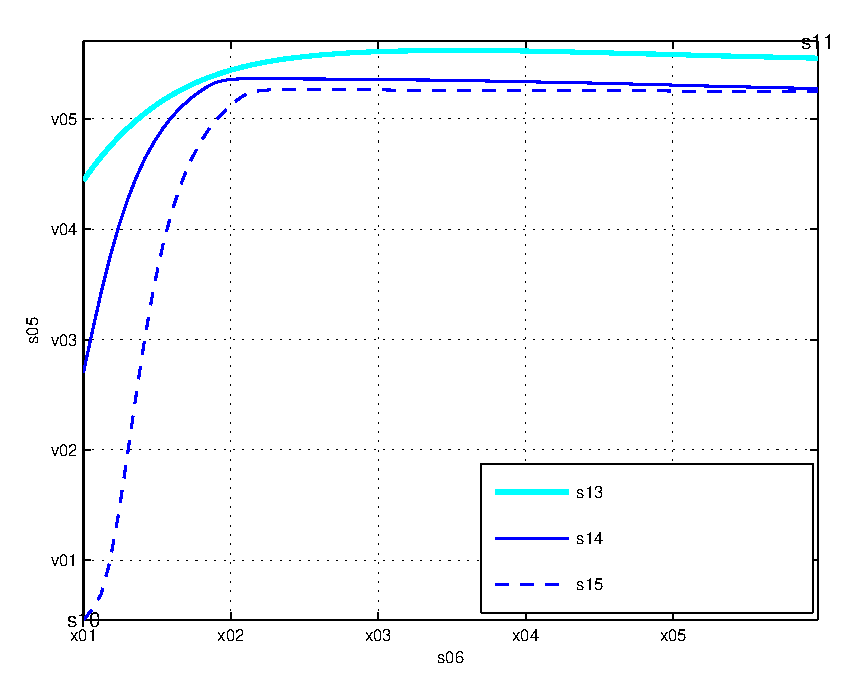
\includegraphics{fig_opt_thr_vs_SNR_AWGN.eps}}%
%\end{psfrags}%
%
% End fig_opt_thr_vs_SNR_AWGN.tex

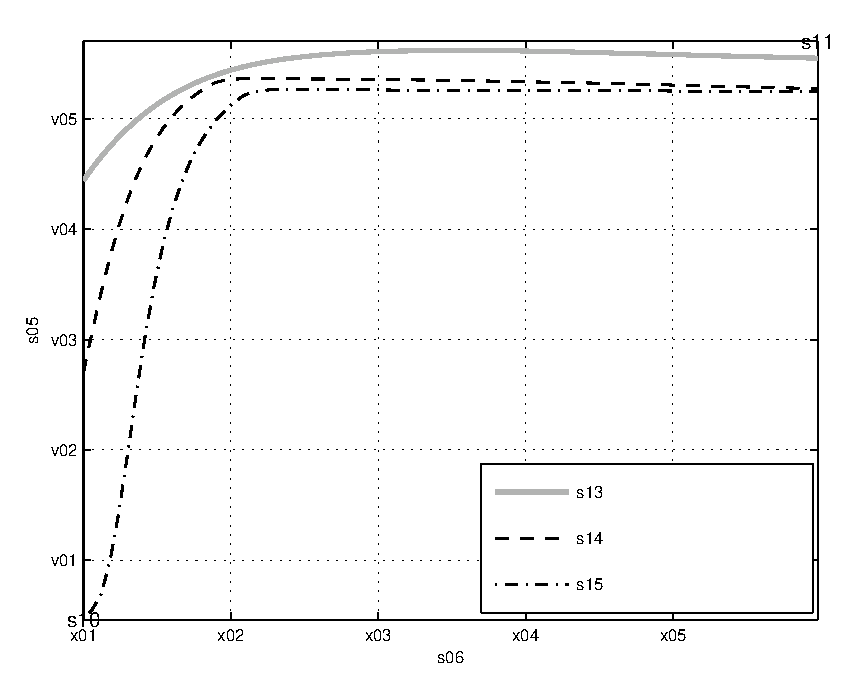
\includegraphics[width= \figscale]{figures/fig_opt_thr_vs_SNR_AWGN}
}
\caption{\tc{Secondary throughput versus $\snrrcvd$ with $\tau\sub{est} = \SI{5}{ms}$ for the deterministic channel.}}
\label{fig_IS:optT_snr}
%\vspace{-0.7cm}
\end{figure}

Hereafter, the theoretical expressions are considered for the analysis, in addition, the IS is operated at the suitable sensing time. Next, the variation in the achievable throughput $\rs(\test, \ttsen)$ against the received signal to noise ratio $\snrrcvd$ at the ST with $\test = \SI{5}{ms}$ is considered, \tc{refer to} \figurename~\ref{fig_IS:optT_snr}. For $\snrrcvd < -\SI{10}{dB}$, the estimation model incurs a significant performance loss. This clearly reveals that the ideal model overestimates the performance of the IS. \tc{From the previous discussion, it is concluded that the inclusion of the average and the outage constraints (depicted by the proposed framework) precisely tackles the uncertainty in the interference at the PR, arising due to channel estimation, without considerably degrading the performance of the IS.}


Upon maximizing the secondary throughput, it is interesting to analyze the variation of the secondary throughput with the estimation time. Corresponding to the estimation model, \figurename~\ref{fig_IS:EST} illustrates a tradeoff among the estimation time, the sensing time and the secondary throughput. \tc{From \figurename~\ref{fig_IS:EST}, it can be noticed that the function $\rs(\test, \tsen)$ is well-behaved in the region $0 < \test \le \tsen \le T$ and consists of a global maximum, yielding the achievable secondary throughput.


\begin{figure}[!h]
\centering
\subfloat[]{
%% Add psfrag entries
\resizebox{\resizescale}{!}{%
% This file is generated by the MATLAB m-file laprint.m. It can be included
% into LaTeX documents using the packages graphicx, color and psfrag.
% It is accompanied by a postscript file. A sample LaTeX file is:
%    \documentclass{article}\usepackage{graphicx,color,psfrag}
%    \begin{document}% This file is generated by the MATLAB m-file laprint.m. It can be included
% into LaTeX documents using the packages graphicx, color and psfrag.
% It is accompanied by a postscript file. A sample LaTeX file is:
%    \documentclass{article}\usepackage{graphicx,color,psfrag}
%    \begin{document}% This file is generated by the MATLAB m-file laprint.m. It can be included
% into LaTeX documents using the packages graphicx, color and psfrag.
% It is accompanied by a postscript file. A sample LaTeX file is:
%    \documentclass{article}\usepackage{graphicx,color,psfrag}
%    \begin{document}\input{fig_opt_thr_vs_est_time_sen_time_ac_AWGN}\end{document}
% See http://www.mathworks.de/matlabcentral/fileexchange/loadFile.do?objectId=4638
% for recent versions of laprint.m.
%
% created by:           LaPrint version 3.16 (13.9.2004)
% created on:           11-Nov-2015 10:11:34
% eps bounding box:     16 cm x 12 cm
% comment:              
%
%\begin{psfrags}%
%\psfragscanon%
%
% text strings:
\psfrag{s02}[b][b]{\fontsize{8}{12}\fontseries{m}\mathversion{normal}\fontshape{n}\selectfont \color[rgb]{0,0,0}\setlength{\tabcolsep}{0pt}\begin{tabular}{c}$\trs(\test,\tsen)$ [bits/sec/Hz]\end{tabular}}%
\psfrag{s03}[lt][lt]{\fontsize{8}{12}\fontseries{m}\mathversion{normal}\fontshape{n}\selectfont \color[rgb]{0,0,0}\setlength{\tabcolsep}{0pt}\begin{tabular}{l}$\tsen$ [ms]\end{tabular}}%
\psfrag{s04}[rt][rt]{\fontsize{8}{12}\fontseries{m}\mathversion{normal}\fontshape{n}\selectfont \color[rgb]{0,0,0}\setlength{\tabcolsep}{0pt}\begin{tabular}{r}$\test$ [ms]\end{tabular}}%
%
% axes font properties:
\fontsize{8}{12}\fontseries{m}\mathversion{normal}%
\fontshape{n}\selectfont%
%
% xticklabels:
\psfrag{x01}[t][t]{0}%
\psfrag{x02}[t][t]{5}%
\psfrag{x03}[t][t]{10}%
\psfrag{x04}[t][t]{15}%
\psfrag{x05}[t][t]{20}%
\psfrag{x06}[t][t]{25}%
%
% yticklabels:
\psfrag{v01}[r][r]{0}%
\psfrag{v02}[r][r]{5}%
\psfrag{v03}[r][r]{10}%
%
% zticklabels:
\psfrag{z01}[r][r]{0}%
\psfrag{z02}[r][r]{0.5}%
\psfrag{z03}[r][r]{1}%
\psfrag{z04}[r][r]{1.5}%
\psfrag{z05}[r][r]{2}%
\psfrag{z06}[r][r]{2.5}%
\psfrag{z07}[r][r]{3}%
%
% Figure:
%\resizebox{8cm}{!}{\includegraphics{fig_opt_thr_vs_est_time_sen_time_ac_AWGN.eps}}%
%\end{psfrags}%
%
% End fig_opt_thr_vs_est_time_sen_time_ac_AWGN.tex
\end{document}
% See http://www.mathworks.de/matlabcentral/fileexchange/loadFile.do?objectId=4638
% for recent versions of laprint.m.
%
% created by:           LaPrint version 3.16 (13.9.2004)
% created on:           11-Nov-2015 10:11:34
% eps bounding box:     16 cm x 12 cm
% comment:              
%
%\begin{psfrags}%
%\psfragscanon%
%
% text strings:
\psfrag{s02}[b][b]{\fontsize{8}{12}\fontseries{m}\mathversion{normal}\fontshape{n}\selectfont \color[rgb]{0,0,0}\setlength{\tabcolsep}{0pt}\begin{tabular}{c}$\trs(\test,\tsen)$ [bits/sec/Hz]\end{tabular}}%
\psfrag{s03}[lt][lt]{\fontsize{8}{12}\fontseries{m}\mathversion{normal}\fontshape{n}\selectfont \color[rgb]{0,0,0}\setlength{\tabcolsep}{0pt}\begin{tabular}{l}$\tsen$ [ms]\end{tabular}}%
\psfrag{s04}[rt][rt]{\fontsize{8}{12}\fontseries{m}\mathversion{normal}\fontshape{n}\selectfont \color[rgb]{0,0,0}\setlength{\tabcolsep}{0pt}\begin{tabular}{r}$\test$ [ms]\end{tabular}}%
%
% axes font properties:
\fontsize{8}{12}\fontseries{m}\mathversion{normal}%
\fontshape{n}\selectfont%
%
% xticklabels:
\psfrag{x01}[t][t]{0}%
\psfrag{x02}[t][t]{5}%
\psfrag{x03}[t][t]{10}%
\psfrag{x04}[t][t]{15}%
\psfrag{x05}[t][t]{20}%
\psfrag{x06}[t][t]{25}%
%
% yticklabels:
\psfrag{v01}[r][r]{0}%
\psfrag{v02}[r][r]{5}%
\psfrag{v03}[r][r]{10}%
%
% zticklabels:
\psfrag{z01}[r][r]{0}%
\psfrag{z02}[r][r]{0.5}%
\psfrag{z03}[r][r]{1}%
\psfrag{z04}[r][r]{1.5}%
\psfrag{z05}[r][r]{2}%
\psfrag{z06}[r][r]{2.5}%
\psfrag{z07}[r][r]{3}%
%
% Figure:
%\resizebox{8cm}{!}{\includegraphics{fig_opt_thr_vs_est_time_sen_time_ac_AWGN.eps}}%
%\end{psfrags}%
%
% End fig_opt_thr_vs_est_time_sen_time_ac_AWGN.tex
\end{document}
% See http://www.mathworks.de/matlabcentral/fileexchange/loadFile.do?objectId=4638
% for recent versions of laprint.m.
%
% created by:           LaPrint version 3.16 (13.9.2004)
% created on:           11-Nov-2015 10:11:34
% eps bounding box:     16 cm x 12 cm
% comment:              
%
%\begin{psfrags}%
%\psfragscanon%
%
% text strings:
\psfrag{s02}[b][b]{\fontsize{8}{12}\fontseries{m}\mathversion{normal}\fontshape{n}\selectfont \color[rgb]{0,0,0}\setlength{\tabcolsep}{0pt}\begin{tabular}{c}$\trs(\test,\tsen)$ [bits/sec/Hz]\end{tabular}}%
\psfrag{s03}[lt][lt]{\fontsize{8}{12}\fontseries{m}\mathversion{normal}\fontshape{n}\selectfont \color[rgb]{0,0,0}\setlength{\tabcolsep}{0pt}\begin{tabular}{l}$\tsen$ [ms]\end{tabular}}%
\psfrag{s04}[rt][rt]{\fontsize{8}{12}\fontseries{m}\mathversion{normal}\fontshape{n}\selectfont \color[rgb]{0,0,0}\setlength{\tabcolsep}{0pt}\begin{tabular}{r}$\test$ [ms]\end{tabular}}%
%
% axes font properties:
\fontsize{8}{12}\fontseries{m}\mathversion{normal}%
\fontshape{n}\selectfont%
%
% xticklabels:
\psfrag{x01}[t][t]{0}%
\psfrag{x02}[t][t]{5}%
\psfrag{x03}[t][t]{10}%
\psfrag{x04}[t][t]{15}%
\psfrag{x05}[t][t]{20}%
\psfrag{x06}[t][t]{25}%
%
% yticklabels:
\psfrag{v01}[r][r]{0}%
\psfrag{v02}[r][r]{5}%
\psfrag{v03}[r][r]{10}%
%
% zticklabels:
\psfrag{z01}[r][r]{0}%
\psfrag{z02}[r][r]{0.5}%
\psfrag{z03}[r][r]{1}%
\psfrag{z04}[r][r]{1.5}%
\psfrag{z05}[r][r]{2}%
\psfrag{z06}[r][r]{2.5}%
\psfrag{z07}[r][r]{3}%
%
% Figure:
%\resizebox{8cm}{!}{\includegraphics{fig_opt_thr_vs_est_time_sen_time_ac_AWGN.eps}}%
%\end{psfrags}%
%
% End fig_opt_thr_vs_est_time_sen_time_ac_AWGN.tex

\centering
\begin{tikzpicture}[scale=1]
\node[anchor=south west,inner sep=0] (image) at (0,0)
{
\includegraphics[width= \figscale]{figures/fig_opt_thr_vs_est_time_sen_time_ac_AWGN}
};
\begin{scope}[x={(image.south east)},y={(image.north west)}]
%\draw[black,->] (0.6,0.44) node[above=0.0,  font=\small] {$\mpd \in \{0.05,0.10,0.15\}$} -- (0.56,0.33);
\draw[black,->] (0.389,0.83) -- (0.389,0.656);
\node[draw=none, font=\footnotesize] at (0.389, 0.86) {$\rs(\ttest, \ttsen)$};

%\draw[help lines,xstep=.1,ystep=.1] (0,0) grid (1,1);
%\foreach \x in {0,1,...,9} { \node [anchor=north] at (\x/10,0) {0.\x}; }
%\foreach \y in {0,1,...,9} { \node [anchor=east] at (0,\y/10) {0.\y}; }
\end{scope}
\end{tikzpicture}
}

\label{fig_IS:EST_ac}}
\hfil
\subfloat[]{
%% Add psfrag entries
\resizebox{\resizescale}{!}{%
% This file is generated by the MATLAB m-file laprint.m. It can be included
% into LaTeX documents using the packages graphicx, color and psfrag.
% It is accompanied by a postscript file. A sample LaTeX file is:
%    \documentclass{article}\usepackage{graphicx,color,psfrag}
%    \begin{document}% This file is generated by the MATLAB m-file laprint.m. It can be included
% into LaTeX documents using the packages graphicx, color and psfrag.
% It is accompanied by a postscript file. A sample LaTeX file is:
%    \documentclass{article}\usepackage{graphicx,color,psfrag}
%    \begin{document}% This file is generated by the MATLAB m-file laprint.m. It can be included
% into LaTeX documents using the packages graphicx, color and psfrag.
% It is accompanied by a postscript file. A sample LaTeX file is:
%    \documentclass{article}\usepackage{graphicx,color,psfrag}
%    \begin{document}\input{fig_opt_thr_vs_est_time_sen_time_oc_AWGN}\end{document}
% See http://www.mathworks.de/matlabcentral/fileexchange/loadFile.do?objectId=4638
% for recent versions of laprint.m.
%
% created by:           LaPrint version 3.16 (13.9.2004)
% created on:           11-Nov-2015 10:11:33
% eps bounding box:     16 cm x 12 cm
% comment:              
%
%\begin{psfrags}%
%\psfragscanon%
%
% text strings:
\psfrag{s02}[b][b]{\fontsize{8}{12}\fontseries{m}\mathversion{normal}\fontshape{n}\selectfont \color[rgb]{0,0,0}\setlength{\tabcolsep}{0pt}\begin{tabular}{c}$\trs(\test,\tsen)$ [bits/sec/Hz]\end{tabular}}%
\psfrag{s03}[lt][lt]{\fontsize{8}{12}\fontseries{m}\mathversion{normal}\fontshape{n}\selectfont \color[rgb]{0,0,0}\setlength{\tabcolsep}{0pt}\begin{tabular}{l}$\tsen$ [ms]\end{tabular}}%
\psfrag{s04}[rt][rt]{\fontsize{8}{12}\fontseries{m}\mathversion{normal}\fontshape{n}\selectfont \color[rgb]{0,0,0}\setlength{\tabcolsep}{0pt}\begin{tabular}{r}$\test$ [ms]\end{tabular}}%
%
% axes font properties:
\fontsize{8}{12}\fontseries{m}\mathversion{normal}%
\fontshape{n}\selectfont%
%
% xticklabels:
\psfrag{x01}[t][t]{0}%
\psfrag{x02}[t][t]{5}%
\psfrag{x03}[t][t]{10}%
\psfrag{x04}[t][t]{15}%
\psfrag{x05}[t][t]{20}%
\psfrag{x06}[t][t]{25}%
%
% yticklabels:
\psfrag{v01}[r][r]{0}%
\psfrag{v02}[r][r]{5}%
\psfrag{v03}[r][r]{10}%
%
% zticklabels:
\psfrag{z01}[r][r]{0}%
\psfrag{z02}[r][r]{0.5}%
\psfrag{z03}[r][r]{1}%
\psfrag{z04}[r][r]{1.5}%
\psfrag{z05}[r][r]{2}%
\psfrag{z06}[r][r]{2.5}%
\psfrag{z07}[r][r]{3}%
%
% Figure:
%\resizebox{8cm}{!}{\includegraphics{fig_opt_thr_vs_est_time_sen_time_oc_AWGN.eps}}%
%\end{psfrags}%
%
% End fig_opt_thr_vs_est_time_sen_time_oc_AWGN.tex
\end{document}
% See http://www.mathworks.de/matlabcentral/fileexchange/loadFile.do?objectId=4638
% for recent versions of laprint.m.
%
% created by:           LaPrint version 3.16 (13.9.2004)
% created on:           11-Nov-2015 10:11:33
% eps bounding box:     16 cm x 12 cm
% comment:              
%
%\begin{psfrags}%
%\psfragscanon%
%
% text strings:
\psfrag{s02}[b][b]{\fontsize{8}{12}\fontseries{m}\mathversion{normal}\fontshape{n}\selectfont \color[rgb]{0,0,0}\setlength{\tabcolsep}{0pt}\begin{tabular}{c}$\trs(\test,\tsen)$ [bits/sec/Hz]\end{tabular}}%
\psfrag{s03}[lt][lt]{\fontsize{8}{12}\fontseries{m}\mathversion{normal}\fontshape{n}\selectfont \color[rgb]{0,0,0}\setlength{\tabcolsep}{0pt}\begin{tabular}{l}$\tsen$ [ms]\end{tabular}}%
\psfrag{s04}[rt][rt]{\fontsize{8}{12}\fontseries{m}\mathversion{normal}\fontshape{n}\selectfont \color[rgb]{0,0,0}\setlength{\tabcolsep}{0pt}\begin{tabular}{r}$\test$ [ms]\end{tabular}}%
%
% axes font properties:
\fontsize{8}{12}\fontseries{m}\mathversion{normal}%
\fontshape{n}\selectfont%
%
% xticklabels:
\psfrag{x01}[t][t]{0}%
\psfrag{x02}[t][t]{5}%
\psfrag{x03}[t][t]{10}%
\psfrag{x04}[t][t]{15}%
\psfrag{x05}[t][t]{20}%
\psfrag{x06}[t][t]{25}%
%
% yticklabels:
\psfrag{v01}[r][r]{0}%
\psfrag{v02}[r][r]{5}%
\psfrag{v03}[r][r]{10}%
%
% zticklabels:
\psfrag{z01}[r][r]{0}%
\psfrag{z02}[r][r]{0.5}%
\psfrag{z03}[r][r]{1}%
\psfrag{z04}[r][r]{1.5}%
\psfrag{z05}[r][r]{2}%
\psfrag{z06}[r][r]{2.5}%
\psfrag{z07}[r][r]{3}%
%
% Figure:
%\resizebox{8cm}{!}{\includegraphics{fig_opt_thr_vs_est_time_sen_time_oc_AWGN.eps}}%
%\end{psfrags}%
%
% End fig_opt_thr_vs_est_time_sen_time_oc_AWGN.tex
\end{document}
% See http://www.mathworks.de/matlabcentral/fileexchange/loadFile.do?objectId=4638
% for recent versions of laprint.m.
%
% created by:           LaPrint version 3.16 (13.9.2004)
% created on:           11-Nov-2015 10:11:33
% eps bounding box:     16 cm x 12 cm
% comment:              
%
%\begin{psfrags}%
%\psfragscanon%
%
% text strings:
\psfrag{s02}[b][b]{\fontsize{8}{12}\fontseries{m}\mathversion{normal}\fontshape{n}\selectfont \color[rgb]{0,0,0}\setlength{\tabcolsep}{0pt}\begin{tabular}{c}$\trs(\test,\tsen)$ [bits/sec/Hz]\end{tabular}}%
\psfrag{s03}[lt][lt]{\fontsize{8}{12}\fontseries{m}\mathversion{normal}\fontshape{n}\selectfont \color[rgb]{0,0,0}\setlength{\tabcolsep}{0pt}\begin{tabular}{l}$\tsen$ [ms]\end{tabular}}%
\psfrag{s04}[rt][rt]{\fontsize{8}{12}\fontseries{m}\mathversion{normal}\fontshape{n}\selectfont \color[rgb]{0,0,0}\setlength{\tabcolsep}{0pt}\begin{tabular}{r}$\test$ [ms]\end{tabular}}%
%
% axes font properties:
\fontsize{8}{12}\fontseries{m}\mathversion{normal}%
\fontshape{n}\selectfont%
%
% xticklabels:
\psfrag{x01}[t][t]{0}%
\psfrag{x02}[t][t]{5}%
\psfrag{x03}[t][t]{10}%
\psfrag{x04}[t][t]{15}%
\psfrag{x05}[t][t]{20}%
\psfrag{x06}[t][t]{25}%
%
% yticklabels:
\psfrag{v01}[r][r]{0}%
\psfrag{v02}[r][r]{5}%
\psfrag{v03}[r][r]{10}%
%
% zticklabels:
\psfrag{z01}[r][r]{0}%
\psfrag{z02}[r][r]{0.5}%
\psfrag{z03}[r][r]{1}%
\psfrag{z04}[r][r]{1.5}%
\psfrag{z05}[r][r]{2}%
\psfrag{z06}[r][r]{2.5}%
\psfrag{z07}[r][r]{3}%
%
% Figure:
%\resizebox{8cm}{!}{\includegraphics{fig_opt_thr_vs_est_time_sen_time_oc_AWGN.eps}}%
%\end{psfrags}%
%
% End fig_opt_thr_vs_est_time_sen_time_oc_AWGN.tex

\centering
\begin{tikzpicture}[scale=1]
\node[anchor=south west,inner sep=0] (image) at (0,0)
{
\includegraphics[width= \figscale]{figures/fig_opt_thr_vs_est_time_sen_time_oc_AWGN}
};
\begin{scope}[x={(image.south east)},y={(image.north west)}]
%\draw[black,->] (0.6,0.44) node[above=0.0,  font=\small] {$\mpd \in \{0.05,0.10,0.15\}$} -- (0.56,0.33);
\draw[black,->] (0.353,0.83) -- (0.353,0.699);
\node[draw=none, font=\footnotesize] at (0.353, 0.86) {$\rs(\ttest, \ttsen)$};

%\draw[help lines,xstep=.1,ystep=.1] (0,0) grid (1,1);
%\foreach \x in {0,1,...,9} { \node [anchor=north] at (\x/10,0) {0.\x}; }
%\foreach \y in {0,1,...,9} { \node [anchor=east] at (0,\y/10) {0.\y}; }
\end{scope}
\end{tikzpicture}
}
\label{fig_IS:EST_oc}}
\caption{\tc{Estimation-sensing-throughput tradeoff for the estimation model for (a) average constraint and (b) outage constraint with $\mpd = 0.05$.}}
\label{fig_IS:EST}
%\vspace{-0.7cm}
\end{figure}

This tradeoff depicted by the proposed framework can be explained from the fact that low values of the estimation time result in large variations in $\epd$.} To counteract and satisfy the average and the outage constraints, the corresponding thresholds shift to a lower value. This causes an increase in $\pfa$, thereby increasing the sensing-throughput curvature. As a result, the suitable sensing time is obtained at a higher value. However, beyond a certain value ($\ttest$), a further increase in the estimation time slightly contributes to the performance improvement and largely consumes the time resources. As a consequence to the estimation-sensing-throughput tradeoff, the suitable estimation time that yields an achievable throughput $\trs(\ttest,\ttsen)$ is determined.


\begin{figure}[t]
\centering
%\subfloat[]{
\resizebox{\resizescale}{!}{%
% This file is generated by the MATLAB m-file laprint.m. It can be included
% into LaTeX documents using the packages graphicx, color and psfrag.
% It is accompanied by a postscript file. A sample LaTeX file is:
%    \documentclass{article}\usepackage{graphicx,color,psfrag}
%    \begin{document}% This file is generated by the MATLAB m-file laprint.m. It can be included
% into LaTeX documents using the packages graphicx, color and psfrag.
% It is accompanied by a postscript file. A sample LaTeX file is:
%    \documentclass{article}\usepackage{graphicx,color,psfrag}
%    \begin{document}% This file is generated by the MATLAB m-file laprint.m. It can be included
% into LaTeX documents using the packages graphicx, color and psfrag.
% It is accompanied by a postscript file. A sample LaTeX file is:
%    \documentclass{article}\usepackage{graphicx,color,psfrag}
%    \begin{document}\input{fig_P_d_vs_est_time_diff_mu_AWGN}\end{document}
% See http://www.mathworks.de/matlabcentral/fileexchange/loadFile.do?objectId=4638
% for recent versions of laprint.m.
%
% created by:           LaPrint version 3.16 (13.9.2004)
% created on:           10-Nov-2015 13:50:43
% eps bounding box:     16 cm x 12 cm
% comment:              
%
%\begin{psfrags}%
%\psfragscanon%
%
% text strings:
\psfrag{s05}[b][b]{\fontsize{8}{12}\fontseries{m}\mathversion{normal}\fontshape{n}\selectfont \color[rgb]{0,0,0}\setlength{\tabcolsep}{0pt}\begin{tabular}{c}$\e{\pd}{\pd}$\end{tabular}}%
\psfrag{s06}[t][t]{\fontsize{8}{12}\fontseries{m}\mathversion{normal}\fontshape{n}\selectfont \color[rgb]{0,0,0}\setlength{\tabcolsep}{0pt}\begin{tabular}{c}$\test$ [ms]\end{tabular}}%
\psfrag{s10}[][]{\fontsize{10}{15}\fontseries{m}\mathversion{normal}\fontshape{n}\selectfont \color[rgb]{0,0,0}\setlength{\tabcolsep}{0pt}\begin{tabular}{c} \end{tabular}}%
\psfrag{s11}[][]{\fontsize{10}{15}\fontseries{m}\mathversion{normal}\fontshape{n}\selectfont \color[rgb]{0,0,0}\setlength{\tabcolsep}{0pt}\begin{tabular}{c} \end{tabular}}%
\psfrag{s12}[l][l]{\fontsize{8}{12}\fontseries{m}\mathversion{normal}\fontshape{n}\selectfont \color[rgb]{0,0,0}Corollary 1}%
\psfrag{s13}[l][l]{\fontsize{8}{12}\fontseries{m}\mathversion{normal}\fontshape{n}\selectfont \color[rgb]{0,0,0}IM}%
\psfrag{s14}[l][l]{\fontsize{8}{12}\fontseries{m}\mathversion{normal}\fontshape{n}\selectfont \color[rgb]{0,0,0}EM-AC, Thm. 1}%
\psfrag{s15}[l][l]{\fontsize{8}{12}\fontseries{m}\mathversion{normal}\fontshape{n}\selectfont \color[rgb]{0,0,0}EM-OC, Thm. 2}%
\psfrag{s16}[l][l]{\fontsize{8}{12}\fontseries{m}\mathversion{normal}\fontshape{n}\selectfont \color[rgb]{0,0,0}Corollary 1}%
%
% axes font properties:
\fontsize{8}{12}\fontseries{m}\mathversion{normal}%
\fontshape{n}\selectfont%
%
% xticklabels:
\psfrag{x01}[t][t]{1}%
\psfrag{x02}[t][t]{2}%
\psfrag{x03}[t][t]{3}%
\psfrag{x04}[t][t]{4}%
\psfrag{x05}[t][t]{5}%
\psfrag{x06}[t][t]{6}%
\psfrag{x07}[t][t]{7}%
\psfrag{x08}[t][t]{8}%
\psfrag{x09}[t][t]{9}%
\psfrag{x10}[t][t]{10}%
%
% yticklabels:
\psfrag{v01}[r][r]{0.8}%
\psfrag{v02}[r][r]{0.82}%
\psfrag{v03}[r][r]{0.84}%
\psfrag{v04}[r][r]{0.86}%
\psfrag{v05}[r][r]{0.88}%
\psfrag{v06}[r][r]{0.9}%
\psfrag{v07}[r][r]{0.92}%
\psfrag{v08}[r][r]{0.94}%
\psfrag{v09}[r][r]{0.96}%
\psfrag{v10}[r][r]{0.98}%
\psfrag{v11}[r][r]{1}%
%
% Figure:
%\resizebox{8cm}{!}{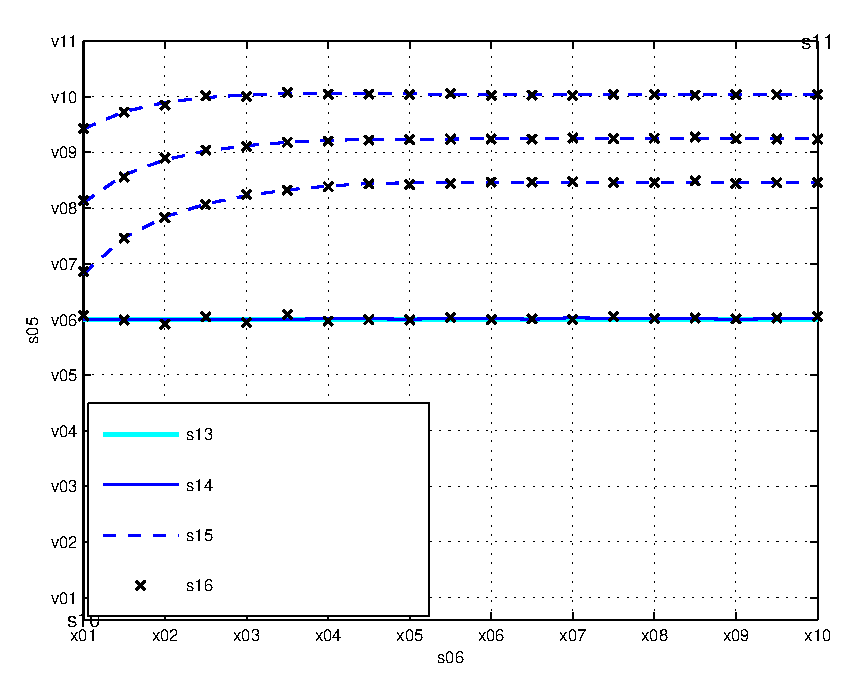
\includegraphics{fig_P_d_vs_est_time_diff_mu_AWGN.eps}}%
%\end{psfrags}%
%
% End fig_P_d_vs_est_time_diff_mu_AWGN.tex
\end{document}
% See http://www.mathworks.de/matlabcentral/fileexchange/loadFile.do?objectId=4638
% for recent versions of laprint.m.
%
% created by:           LaPrint version 3.16 (13.9.2004)
% created on:           10-Nov-2015 13:50:43
% eps bounding box:     16 cm x 12 cm
% comment:              
%
%\begin{psfrags}%
%\psfragscanon%
%
% text strings:
\psfrag{s05}[b][b]{\fontsize{8}{12}\fontseries{m}\mathversion{normal}\fontshape{n}\selectfont \color[rgb]{0,0,0}\setlength{\tabcolsep}{0pt}\begin{tabular}{c}$\e{\pd}{\pd}$\end{tabular}}%
\psfrag{s06}[t][t]{\fontsize{8}{12}\fontseries{m}\mathversion{normal}\fontshape{n}\selectfont \color[rgb]{0,0,0}\setlength{\tabcolsep}{0pt}\begin{tabular}{c}$\test$ [ms]\end{tabular}}%
\psfrag{s10}[][]{\fontsize{10}{15}\fontseries{m}\mathversion{normal}\fontshape{n}\selectfont \color[rgb]{0,0,0}\setlength{\tabcolsep}{0pt}\begin{tabular}{c} \end{tabular}}%
\psfrag{s11}[][]{\fontsize{10}{15}\fontseries{m}\mathversion{normal}\fontshape{n}\selectfont \color[rgb]{0,0,0}\setlength{\tabcolsep}{0pt}\begin{tabular}{c} \end{tabular}}%
\psfrag{s12}[l][l]{\fontsize{8}{12}\fontseries{m}\mathversion{normal}\fontshape{n}\selectfont \color[rgb]{0,0,0}Corollary 1}%
\psfrag{s13}[l][l]{\fontsize{8}{12}\fontseries{m}\mathversion{normal}\fontshape{n}\selectfont \color[rgb]{0,0,0}IM}%
\psfrag{s14}[l][l]{\fontsize{8}{12}\fontseries{m}\mathversion{normal}\fontshape{n}\selectfont \color[rgb]{0,0,0}EM-AC, Thm. 1}%
\psfrag{s15}[l][l]{\fontsize{8}{12}\fontseries{m}\mathversion{normal}\fontshape{n}\selectfont \color[rgb]{0,0,0}EM-OC, Thm. 2}%
\psfrag{s16}[l][l]{\fontsize{8}{12}\fontseries{m}\mathversion{normal}\fontshape{n}\selectfont \color[rgb]{0,0,0}Corollary 1}%
%
% axes font properties:
\fontsize{8}{12}\fontseries{m}\mathversion{normal}%
\fontshape{n}\selectfont%
%
% xticklabels:
\psfrag{x01}[t][t]{1}%
\psfrag{x02}[t][t]{2}%
\psfrag{x03}[t][t]{3}%
\psfrag{x04}[t][t]{4}%
\psfrag{x05}[t][t]{5}%
\psfrag{x06}[t][t]{6}%
\psfrag{x07}[t][t]{7}%
\psfrag{x08}[t][t]{8}%
\psfrag{x09}[t][t]{9}%
\psfrag{x10}[t][t]{10}%
%
% yticklabels:
\psfrag{v01}[r][r]{0.8}%
\psfrag{v02}[r][r]{0.82}%
\psfrag{v03}[r][r]{0.84}%
\psfrag{v04}[r][r]{0.86}%
\psfrag{v05}[r][r]{0.88}%
\psfrag{v06}[r][r]{0.9}%
\psfrag{v07}[r][r]{0.92}%
\psfrag{v08}[r][r]{0.94}%
\psfrag{v09}[r][r]{0.96}%
\psfrag{v10}[r][r]{0.98}%
\psfrag{v11}[r][r]{1}%
%
% Figure:
%\resizebox{8cm}{!}{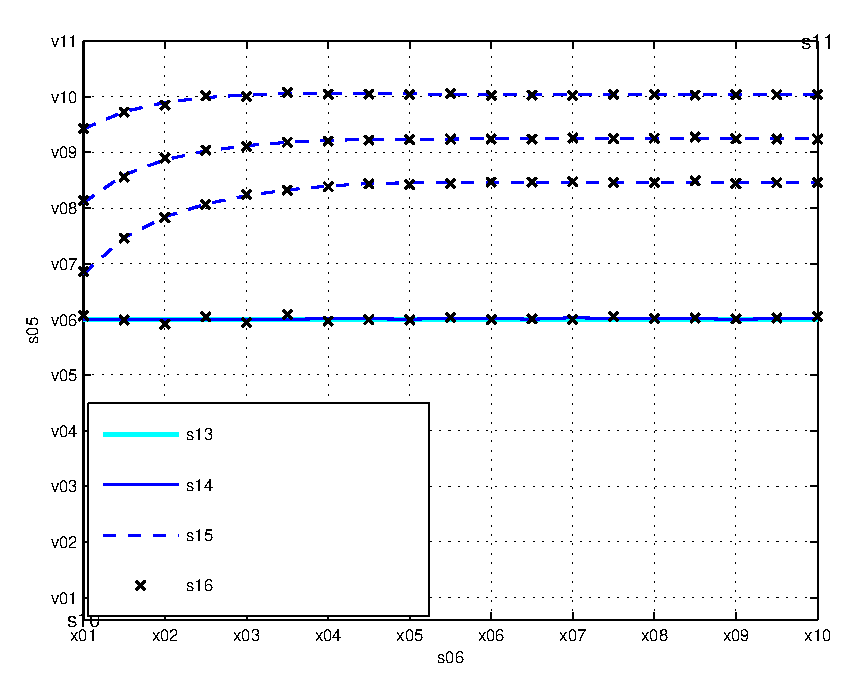
\includegraphics{fig_P_d_vs_est_time_diff_mu_AWGN.eps}}%
%\end{psfrags}%
%
% End fig_P_d_vs_est_time_diff_mu_AWGN.tex
\end{document}
% See http://www.mathworks.de/matlabcentral/fileexchange/loadFile.do?objectId=4638
% for recent versions of laprint.m.
%
% created by:           LaPrint version 3.16 (13.9.2004)
% created on:           10-Nov-2015 13:50:43
% eps bounding box:     16 cm x 12 cm
% comment:              
%
%\begin{psfrags}%
%\psfragscanon%
%
% text strings:
\psfrag{s05}[b][b]{\fontsize{8}{12}\fontseries{m}\mathversion{normal}\fontshape{n}\selectfont \color[rgb]{0,0,0}\setlength{\tabcolsep}{0pt}\begin{tabular}{c}$\e{\pd}{\pd}$\end{tabular}}%
\psfrag{s06}[t][t]{\fontsize{8}{12}\fontseries{m}\mathversion{normal}\fontshape{n}\selectfont \color[rgb]{0,0,0}\setlength{\tabcolsep}{0pt}\begin{tabular}{c}$\test$ [ms]\end{tabular}}%
\psfrag{s10}[][]{\fontsize{10}{15}\fontseries{m}\mathversion{normal}\fontshape{n}\selectfont \color[rgb]{0,0,0}\setlength{\tabcolsep}{0pt}\begin{tabular}{c} \end{tabular}}%
\psfrag{s11}[][]{\fontsize{10}{15}\fontseries{m}\mathversion{normal}\fontshape{n}\selectfont \color[rgb]{0,0,0}\setlength{\tabcolsep}{0pt}\begin{tabular}{c} \end{tabular}}%
\psfrag{s12}[l][l]{\fontsize{8}{12}\fontseries{m}\mathversion{normal}\fontshape{n}\selectfont \color[rgb]{0,0,0}Corollary 1}%
\psfrag{s13}[l][l]{\fontsize{8}{12}\fontseries{m}\mathversion{normal}\fontshape{n}\selectfont \color[rgb]{0,0,0}IM}%
\psfrag{s14}[l][l]{\fontsize{8}{12}\fontseries{m}\mathversion{normal}\fontshape{n}\selectfont \color[rgb]{0,0,0}EM-AC, Thm. 1}%
\psfrag{s15}[l][l]{\fontsize{8}{12}\fontseries{m}\mathversion{normal}\fontshape{n}\selectfont \color[rgb]{0,0,0}EM-OC, Thm. 2}%
\psfrag{s16}[l][l]{\fontsize{8}{12}\fontseries{m}\mathversion{normal}\fontshape{n}\selectfont \color[rgb]{0,0,0}Corollary 1}%
%
% axes font properties:
\fontsize{8}{12}\fontseries{m}\mathversion{normal}%
\fontshape{n}\selectfont%
%
% xticklabels:
\psfrag{x01}[t][t]{1}%
\psfrag{x02}[t][t]{2}%
\psfrag{x03}[t][t]{3}%
\psfrag{x04}[t][t]{4}%
\psfrag{x05}[t][t]{5}%
\psfrag{x06}[t][t]{6}%
\psfrag{x07}[t][t]{7}%
\psfrag{x08}[t][t]{8}%
\psfrag{x09}[t][t]{9}%
\psfrag{x10}[t][t]{10}%
%
% yticklabels:
\psfrag{v01}[r][r]{0.8}%
\psfrag{v02}[r][r]{0.82}%
\psfrag{v03}[r][r]{0.84}%
\psfrag{v04}[r][r]{0.86}%
\psfrag{v05}[r][r]{0.88}%
\psfrag{v06}[r][r]{0.9}%
\psfrag{v07}[r][r]{0.92}%
\psfrag{v08}[r][r]{0.94}%
\psfrag{v09}[r][r]{0.96}%
\psfrag{v10}[r][r]{0.98}%
\psfrag{v11}[r][r]{1}%
%
% Figure:
%\resizebox{8cm}{!}{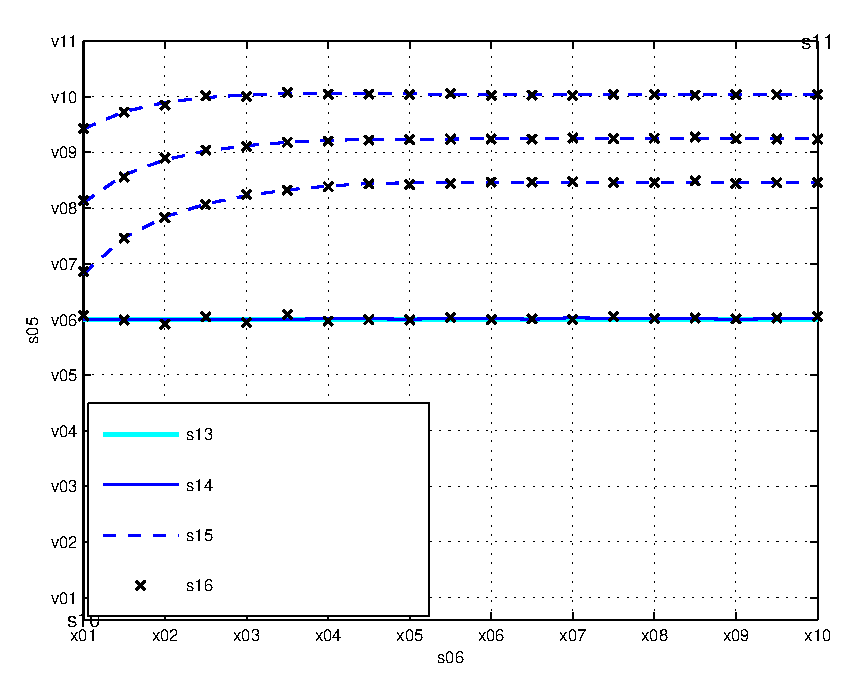
\includegraphics{fig_P_d_vs_est_time_diff_mu_AWGN.eps}}%
%\end{psfrags}%
%
% End fig_P_d_vs_est_time_diff_mu_AWGN.tex

\begin{tikzpicture}[scale=1]
\node[anchor=south west,inner sep=0] (image) at (0,0)
{
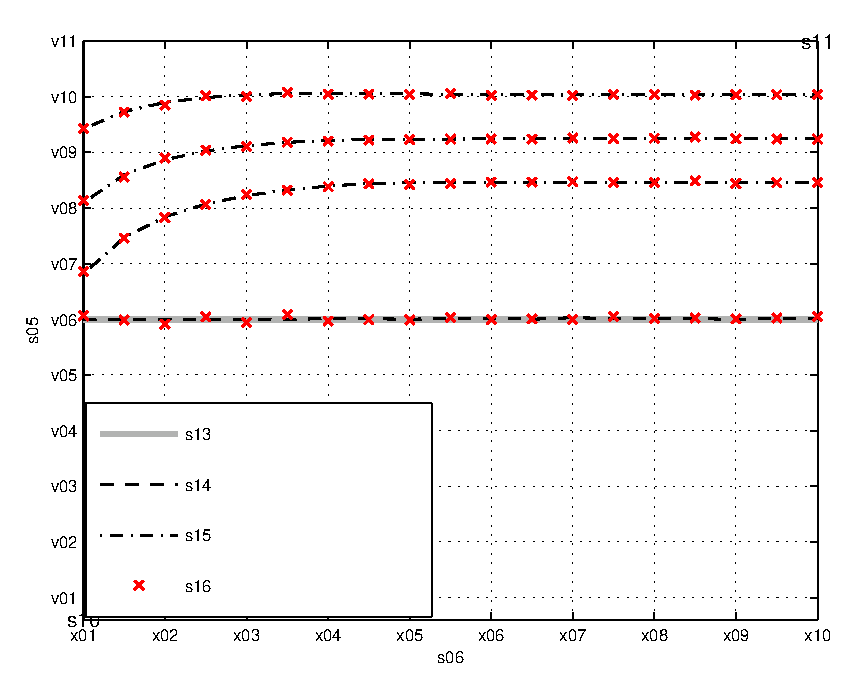
\includegraphics[width = \figscale]{figures/fig_P_d_vs_est_time_diff_mu_AWGN}
};
\begin{scope}[x={(image.south east)},y={(image.north west)}]
\draw[black,->] (0.25,0.68) -- (0.14,0.92);
\node[draw=none,font=\footnotesize] at (0.28,0.62) {$\mpd \in \{0.05,0.10,0.15\}$};

%\draw[help lines,xstep=.1,ystep=.1] (0,0) grid (1,1);
%\foreach \x in {0,1,...,9} { \node [anchor=north] at (\x/10,0) {0.\x}; }
%\foreach \y in {0,1,...,9} { \node [anchor=east] at (0,\y/10) {0.\y}; }
\end{scope}
\end{tikzpicture}
}
\caption{Variation of $\e{\epd}{\epd}$ versus the $\test$, where the secondary throughput is maximized over the sensing time, $\trs(\test,\ttsen)$.}
\label{fig_IS:pd_test}%}
\end{figure}



\begin{figure}
\centering
\resizebox{\resizescale}{!}{%
% This file is generated by the MATLAB m-file laprint.m. It can be included
% into LaTeX documents using the packages graphicx, color and psfrag.
% It is accompanied by a postscript file. A sample LaTeX file is:
%    \documentclass{article}\usepackage{graphicx,color,psfrag}
%    \begin{document}% This file is generated by the MATLAB m-file laprint.m. It can be included
% into LaTeX documents using the packages graphicx, color and psfrag.
% It is accompanied by a postscript file. A sample LaTeX file is:
%    \documentclass{article}\usepackage{graphicx,color,psfrag}
%    \begin{document}% This file is generated by the MATLAB m-file laprint.m. It can be included
% into LaTeX documents using the packages graphicx, color and psfrag.
% It is accompanied by a postscript file. A sample LaTeX file is:
%    \documentclass{article}\usepackage{graphicx,color,psfrag}
%    \begin{document}\input{fig_P_f_vs_est_time_diff_mu_AWGN}\end{document}
% See http://www.mathworks.de/matlabcentral/fileexchange/loadFile.do?objectId=4638
% for recent versions of laprint.m.
%
% created by:           LaPrint version 3.16 (13.9.2004)
% created on:           12-Jul-2016 15:03:25
% eps bounding box:     16 cm x 12 cm
% comment:              
%
%\begin{psfrags}%
%\psfragscanon%
%
% text strings:
\psfrag{s05}[b][b]{\fontsize{8}{12}\fontseries{m}\mathversion{normal}\fontshape{n}\selectfont \color[rgb]{0,0,0}\setlength{\tabcolsep}{0pt}\begin{tabular}{c}$\pfa$\end{tabular}}%
\psfrag{s06}[t][t]{\fontsize{8}{12}\fontseries{m}\mathversion{normal}\fontshape{n}\selectfont \color[rgb]{0,0,0}\setlength{\tabcolsep}{0pt}\begin{tabular}{c}$\test$ = [ms]\end{tabular}}%
\psfrag{s10}[][]{\fontsize{10}{15}\fontseries{m}\mathversion{normal}\fontshape{n}\selectfont \color[rgb]{0,0,0}\setlength{\tabcolsep}{0pt}\begin{tabular}{c} \end{tabular}}%
\psfrag{s11}[][]{\fontsize{10}{15}\fontseries{m}\mathversion{normal}\fontshape{n}\selectfont \color[rgb]{0,0,0}\setlength{\tabcolsep}{0pt}\begin{tabular}{c} \end{tabular}}%
\psfrag{s12}[l][l]{\fontsize{8}{12}\fontseries{m}\mathversion{normal}\fontshape{n}\selectfont \color[rgb]{0,0,0}Corollary 1}%
\psfrag{s13}[l][l]{\fontsize{8}{12}\fontseries{m}\mathversion{normal}\fontshape{n}\selectfont \color[rgb]{0,0,0}IM}%
\psfrag{s14}[l][l]{\fontsize{8}{12}\fontseries{m}\mathversion{normal}\fontshape{n}\selectfont \color[rgb]{0,0,0}EM-AC, Problem 1}%
\psfrag{s15}[l][l]{\fontsize{8}{12}\fontseries{m}\mathversion{normal}\fontshape{n}\selectfont \color[rgb]{0,0,0}EM-OC, Problem 2}%
\psfrag{s16}[l][l]{\fontsize{8}{12}\fontseries{m}\mathversion{normal}\fontshape{n}\selectfont \color[rgb]{0,0,0}Corollary 1}%
%
% axes font properties:
\fontsize{8}{12}\fontseries{m}\mathversion{normal}%
\fontshape{n}\selectfont%
%
% xticklabels:
\psfrag{x01}[t][t]{1}%
\psfrag{x02}[t][t]{2}%
\psfrag{x03}[t][t]{3}%
\psfrag{x04}[t][t]{4}%
\psfrag{x05}[t][t]{5}%
\psfrag{x06}[t][t]{6}%
\psfrag{x07}[t][t]{7}%
\psfrag{x08}[t][t]{8}%
\psfrag{x09}[t][t]{9}%
\psfrag{x10}[t][t]{10}%
%
% yticklabels:
\psfrag{v01}[r][r]{$10^{-4}$}%
\psfrag{v02}[r][r]{$10^{-3}$}%
\psfrag{v03}[r][r]{$10^{-2}$}%
\psfrag{v04}[r][r]{$10^{-1}$}%
%
% Figure:
%\resizebox{8cm}{!}{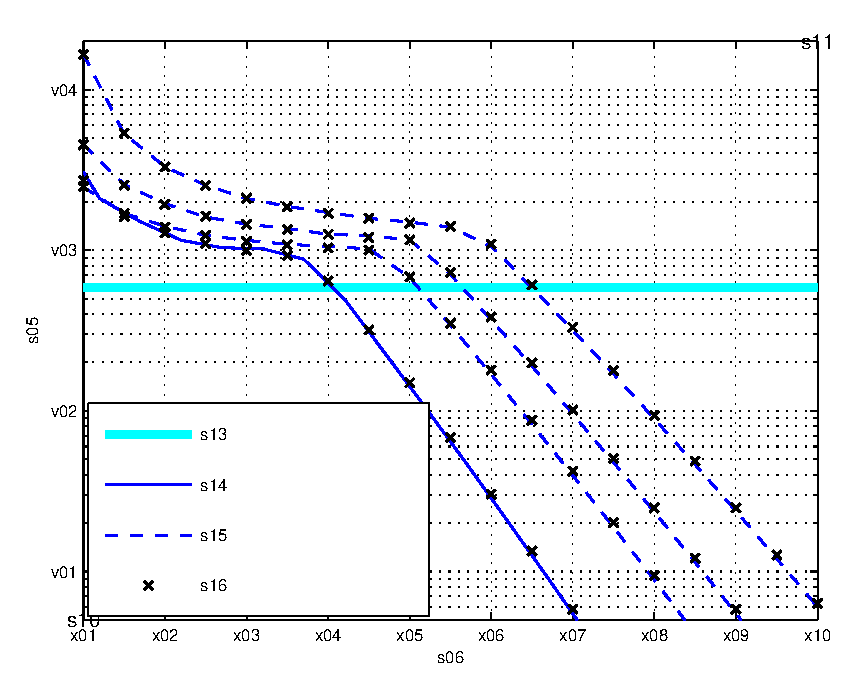
\includegraphics{fig_P_f_vs_est_time_diff_mu_AWGN.eps}}%
%\end{psfrags}%
%
% End fig_P_f_vs_est_time_diff_mu_AWGN.tex
\end{document}
% See http://www.mathworks.de/matlabcentral/fileexchange/loadFile.do?objectId=4638
% for recent versions of laprint.m.
%
% created by:           LaPrint version 3.16 (13.9.2004)
% created on:           12-Jul-2016 15:03:25
% eps bounding box:     16 cm x 12 cm
% comment:              
%
%\begin{psfrags}%
%\psfragscanon%
%
% text strings:
\psfrag{s05}[b][b]{\fontsize{8}{12}\fontseries{m}\mathversion{normal}\fontshape{n}\selectfont \color[rgb]{0,0,0}\setlength{\tabcolsep}{0pt}\begin{tabular}{c}$\pfa$\end{tabular}}%
\psfrag{s06}[t][t]{\fontsize{8}{12}\fontseries{m}\mathversion{normal}\fontshape{n}\selectfont \color[rgb]{0,0,0}\setlength{\tabcolsep}{0pt}\begin{tabular}{c}$\test$ = [ms]\end{tabular}}%
\psfrag{s10}[][]{\fontsize{10}{15}\fontseries{m}\mathversion{normal}\fontshape{n}\selectfont \color[rgb]{0,0,0}\setlength{\tabcolsep}{0pt}\begin{tabular}{c} \end{tabular}}%
\psfrag{s11}[][]{\fontsize{10}{15}\fontseries{m}\mathversion{normal}\fontshape{n}\selectfont \color[rgb]{0,0,0}\setlength{\tabcolsep}{0pt}\begin{tabular}{c} \end{tabular}}%
\psfrag{s12}[l][l]{\fontsize{8}{12}\fontseries{m}\mathversion{normal}\fontshape{n}\selectfont \color[rgb]{0,0,0}Corollary 1}%
\psfrag{s13}[l][l]{\fontsize{8}{12}\fontseries{m}\mathversion{normal}\fontshape{n}\selectfont \color[rgb]{0,0,0}IM}%
\psfrag{s14}[l][l]{\fontsize{8}{12}\fontseries{m}\mathversion{normal}\fontshape{n}\selectfont \color[rgb]{0,0,0}EM-AC, Problem 1}%
\psfrag{s15}[l][l]{\fontsize{8}{12}\fontseries{m}\mathversion{normal}\fontshape{n}\selectfont \color[rgb]{0,0,0}EM-OC, Problem 2}%
\psfrag{s16}[l][l]{\fontsize{8}{12}\fontseries{m}\mathversion{normal}\fontshape{n}\selectfont \color[rgb]{0,0,0}Corollary 1}%
%
% axes font properties:
\fontsize{8}{12}\fontseries{m}\mathversion{normal}%
\fontshape{n}\selectfont%
%
% xticklabels:
\psfrag{x01}[t][t]{1}%
\psfrag{x02}[t][t]{2}%
\psfrag{x03}[t][t]{3}%
\psfrag{x04}[t][t]{4}%
\psfrag{x05}[t][t]{5}%
\psfrag{x06}[t][t]{6}%
\psfrag{x07}[t][t]{7}%
\psfrag{x08}[t][t]{8}%
\psfrag{x09}[t][t]{9}%
\psfrag{x10}[t][t]{10}%
%
% yticklabels:
\psfrag{v01}[r][r]{$10^{-4}$}%
\psfrag{v02}[r][r]{$10^{-3}$}%
\psfrag{v03}[r][r]{$10^{-2}$}%
\psfrag{v04}[r][r]{$10^{-1}$}%
%
% Figure:
%\resizebox{8cm}{!}{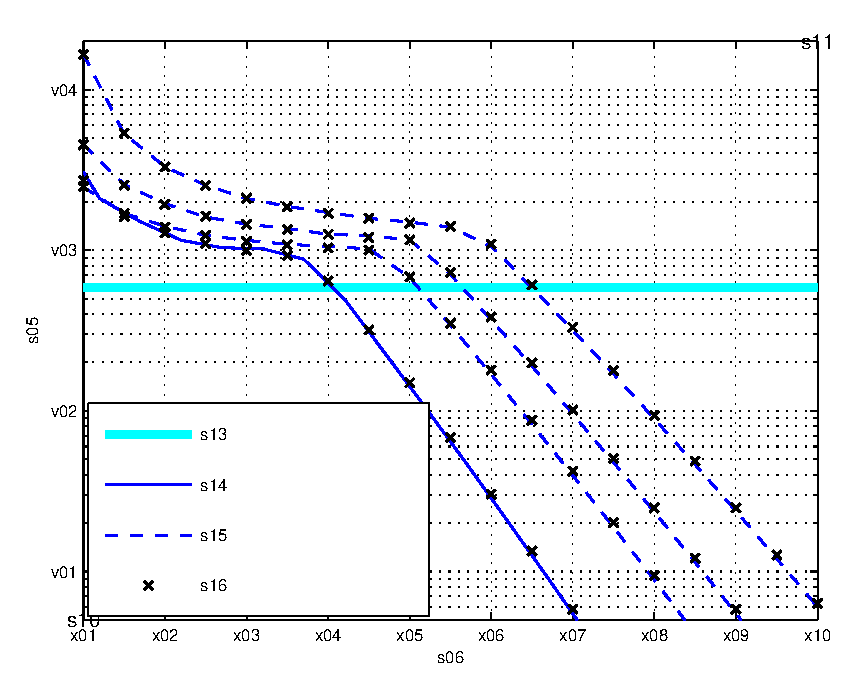
\includegraphics{fig_P_f_vs_est_time_diff_mu_AWGN.eps}}%
%\end{psfrags}%
%
% End fig_P_f_vs_est_time_diff_mu_AWGN.tex
\end{document}
% See http://www.mathworks.de/matlabcentral/fileexchange/loadFile.do?objectId=4638
% for recent versions of laprint.m.
%
% created by:           LaPrint version 3.16 (13.9.2004)
% created on:           12-Jul-2016 15:03:25
% eps bounding box:     16 cm x 12 cm
% comment:              
%
%\begin{psfrags}%
%\psfragscanon%
%
% text strings:
\psfrag{s05}[b][b]{\fontsize{8}{12}\fontseries{m}\mathversion{normal}\fontshape{n}\selectfont \color[rgb]{0,0,0}\setlength{\tabcolsep}{0pt}\begin{tabular}{c}$\pfa$\end{tabular}}%
\psfrag{s06}[t][t]{\fontsize{8}{12}\fontseries{m}\mathversion{normal}\fontshape{n}\selectfont \color[rgb]{0,0,0}\setlength{\tabcolsep}{0pt}\begin{tabular}{c}$\test$ = [ms]\end{tabular}}%
\psfrag{s10}[][]{\fontsize{10}{15}\fontseries{m}\mathversion{normal}\fontshape{n}\selectfont \color[rgb]{0,0,0}\setlength{\tabcolsep}{0pt}\begin{tabular}{c} \end{tabular}}%
\psfrag{s11}[][]{\fontsize{10}{15}\fontseries{m}\mathversion{normal}\fontshape{n}\selectfont \color[rgb]{0,0,0}\setlength{\tabcolsep}{0pt}\begin{tabular}{c} \end{tabular}}%
\psfrag{s12}[l][l]{\fontsize{8}{12}\fontseries{m}\mathversion{normal}\fontshape{n}\selectfont \color[rgb]{0,0,0}Corollary 1}%
\psfrag{s13}[l][l]{\fontsize{8}{12}\fontseries{m}\mathversion{normal}\fontshape{n}\selectfont \color[rgb]{0,0,0}IM}%
\psfrag{s14}[l][l]{\fontsize{8}{12}\fontseries{m}\mathversion{normal}\fontshape{n}\selectfont \color[rgb]{0,0,0}EM-AC, Problem 1}%
\psfrag{s15}[l][l]{\fontsize{8}{12}\fontseries{m}\mathversion{normal}\fontshape{n}\selectfont \color[rgb]{0,0,0}EM-OC, Problem 2}%
\psfrag{s16}[l][l]{\fontsize{8}{12}\fontseries{m}\mathversion{normal}\fontshape{n}\selectfont \color[rgb]{0,0,0}Corollary 1}%
%
% axes font properties:
\fontsize{8}{12}\fontseries{m}\mathversion{normal}%
\fontshape{n}\selectfont%
%
% xticklabels:
\psfrag{x01}[t][t]{1}%
\psfrag{x02}[t][t]{2}%
\psfrag{x03}[t][t]{3}%
\psfrag{x04}[t][t]{4}%
\psfrag{x05}[t][t]{5}%
\psfrag{x06}[t][t]{6}%
\psfrag{x07}[t][t]{7}%
\psfrag{x08}[t][t]{8}%
\psfrag{x09}[t][t]{9}%
\psfrag{x10}[t][t]{10}%
%
% yticklabels:
\psfrag{v01}[r][r]{$10^{-4}$}%
\psfrag{v02}[r][r]{$10^{-3}$}%
\psfrag{v03}[r][r]{$10^{-2}$}%
\psfrag{v04}[r][r]{$10^{-1}$}%
%
% Figure:
%\resizebox{8cm}{!}{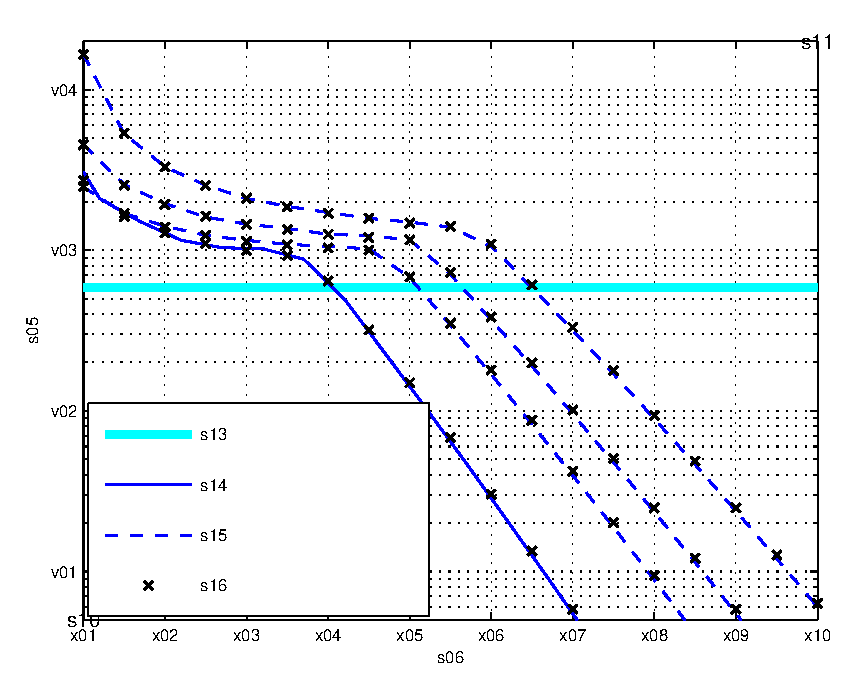
\includegraphics{fig_P_f_vs_est_time_diff_mu_AWGN.eps}}%
%\end{psfrags}%
%
% End fig_P_f_vs_est_time_diff_mu_AWGN.tex

\begin{tikzpicture}[scale=1]
\node[anchor=south west,inner sep=0] (image) at (0,0)
{
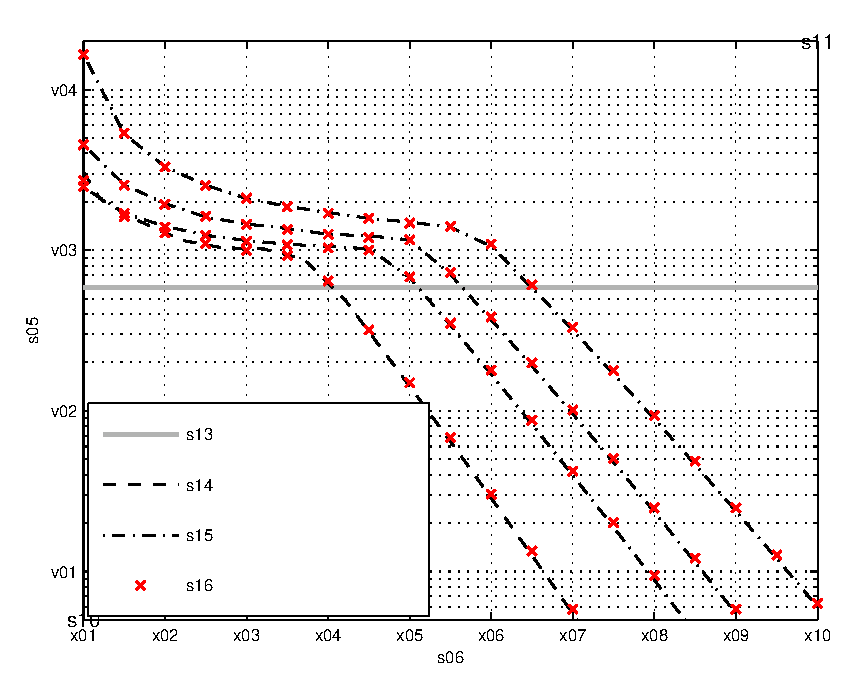
\includegraphics[width = \figscale]{figures/fig_P_f_vs_est_time_diff_mu_AWGN}
};
\begin{scope}[x={(image.south east)},y={(image.north west)}]
%\draw[black,->] (0.6,0.44) node[above=0.0,  font=\small] {$\mpd \in \{0.05,0.10,0.15\}$} -- (0.56,0.33);
\draw[black,->] (0.75,0.47) -- (0.6,0.33);
\node[draw=none, rotate=-50, font=\footnotesize] at (0.78,0.5) {$\mpd \in \{0.05,0.10,0.15\}$};

%\draw[help lines,xstep=.1,ystep=.1] (0,0) grid (1,1);
%\foreach \x in {0,1,...,9} { \node [anchor=north] at (\x/10,0) {0.\x}; }
%\foreach \y in {0,1,...,9} { \node [anchor=east] at (0,\y/10) {0.\y}; }
\end{scope}
\end{tikzpicture}
}
%\vspace{0.3cm}
\caption{Variation of $\pfa$ versus the $\test$, where the secondary throughput is maximized over the sensing time, $\trs(\test,\ttsen)$.}
\label{fig_IS:pf_tsen}%}
%\label{fig_IS:ROC_test}
%\vspace{-0.9cm}
\end{figure}

To procure further insights, the variations of expected $\epd$ and $\pfa$ with the estimation time are studied. From \figurename~\ref{fig_IS:pd_test}, it is observed that the expected $\epd$ corresponding to the outage constraint is strictly above the desired level $\pdd$ for all values of the estimation time. However, for lower values of the estimation time, this margin reduces. This is based on the fact that lower estimation time shifts the probability mass of $\pd$ to a lower value. %On the other side, \figurename~\ref{fig_IS:pf_tsen} illustrates $\pfa$, thereby revealing the performance loss incurred by the IS for the mentioned cases. Clearly, for $\test < \SI{3}{ms}$ depicts a large deviation from the ideal scenario. 
%Besides that, based on the previous discussion, it was analyzed that $\pfa$ accounts for a large contribution to the throughput. 

\tc{According to \figurename~\ref{fig_IS:pf_tsen}, the system notices a considerable improvement in $\pfa$ at small values of $\test$, which saturates for a certain period and falls drastically beyond a certain value. To understand this, it is important to study the dynamics between the estimation and the sensing time. Low $\test$ increases the variations in the detection probability, these variations are compensated by an increase in the suitable sensing time, and vice versa. The performance improves until a maximum ($\ttest$, $\ttsen$) is reached, beyond this, the time resources (allocated in terms of the sensing and the estimation time) contribute more in improving the detector's performance (in terms of $\pfa$ as $\pd$ is already constrained) and less in reducing the variations due to the channel estimation.}%further justification to the variation of $\trs(\test,\ttsen)$ against $\test$ characterized as estimation-sensing-throughput tradeoff depicted in \figurename~\ref{fig_IS:optT_test}.  

\subsection{Summary}
This section investigates the performance of cognitive radio as an interweave system from a deployment perspective. It has been argued that the knowledge of the interacting channels is a key aspect that enables the performance characterization of the interweave system. In this regard, a novel framework that facilitates channel estimation and captures the effect of channel estimation in the system model has been proposed. As a major outcome of the analysis, it has been justified that the existing model, illustrating an ideal scenario, disregards the effects such as time allocation and imperfect channel knowledge encountered by the IS due to the inclusion of channel estimation. In this context, the existing model overestimates the performance of the interweave system, and hence, is less suitable for deployment.

Moreover, it has been clearly identified that the variations induced in the system, specially in the detection probability, cause uncertain interference. Unless controlled, this uncertain interference may severely degrade the performance of the primary system. To overcome this situation, average and outage constraints as primary user constraints have been employed. As a consequence, for the proposed estimation model, novel expressions for the sensing-throughput tradeoff based on the mentioned constraints have been established. More importantly, by analyzing the estimation-sensing-throughput tradeoff, the suitable estimation time and the suitable sensing time that maximize the secondary throughput have been determined.

\section{Research Directions}
\label{sec:RD}
With regard to the performance analysis and the deployment-centric viewpoint towards CR systems emphasized in this chapter, the following extensions or considerations to the proposed framework could be of great interest for future investigations. 


\subsubsection*{In-band Full-duplex}
For instance, this chapter focused only on a \index{CR communication!half duplex}half duplex CR communication, i.e., the \index{CR techniques}CR techniques (which include spectrum sensing and power control) are time-interlaced with the data transmission. Recently, there has been significant advancement concerning the feasibility of \index{CR communication!in-band full duplex}in-band full duplex communication, for a detailed discussion over in-band full duplex communication, please consider \cite{Sab14, Liu15} and the references therein. In this context, the CR communication can be transformed into the in-band full duplex, whereby the CR techniques and the data transmission occurs simultaneously in time and over the same frequency channel. The design challenges and the corresponding performance tradeoffs related to the in-band full duplex CR communication are precisely dealt within \cite{Liao15, Kim15}.

\subsubsection*{Multiple Antennas at ST}
In addition, the performed analysis considers that the ST and the SR are installed with single antenna. As a matter of fact, state-of-the-art standards are mostly equipped with multiple antennas. With an intention of establishing a preliminary analysis involving channel estimation in context of the CR systems, the performance enhancement procured by upgrading the existing spectrum sensing (detector performance) due to the deployment of multiple antennas \cite{Dig07,Tah10}, has been completely neglected in the chapter. Based on a hardware deployment, the authors in \cite{Kaushik16_VTC2} argued that the hardware complexity in context with the CR system escalates with the deployment of multiple antennas, prohibiting the usage of well-known \index{Combining techniques}combining techniques such as equal-gain combining and maximum-ratio combining \cite{Alouini03}. In this regard, non-conventional techniques, such as square-law selector and square-law combiner (following the principle of energy detection) are able to reduce complexity, thereby promoting the feasibility of multiple antennas.

\subsubsection*{Asynchronous Access}
Given the complexity of the underlying problem, impairments due to the \index{Asynchronous access}asynchronous (in time domain) access by the secondary system to the licensed spectrum is left aside throughout the chapter. The asynchronous access is due to the unknown (which can be random also) behaviour of PU traffic. In these circumstances, the assumption concerning the synchronous access (i.e., perfect alignment to the primary system's medium access) becomes invalid. As a consequence, this asynchronous access certainly has an impact on the performance of the CR systems. A careful integration of the asynchronous access to the proposed analysis presents a promising research direction. To tackle this problem, the reader is encouraged to consult the references \cite{Jiang13_, Jiang15}.

%Also, the performance evaluation, presented in the chapter, considers symmetric fading, i.e., the channel gains are subjected to the same value of $m$, which represents \index{Nakagami-$m$ fading}Nakagami-$m$ parameter, characterizing the severity of channel fading. However, depending on the deployment scenario, the derived expressions can be utilized to realize \index{Asymmetric fading}asymmetric fading \cite{Sura08} by substituting different values of $m$ corresponding to different channels. In this regard, the proposed framework can be extended to study the influence of asymmetric fading on the performance.

\subsubsection*{Network-wide perspective}
Finally, the performance analysis in this chapter has been confined to a single of PT, PR and ST and SR, a classical way of illustrating a node-wide perspective of a CR system. The effect of the presence of other PTs and other STs in the network on the performance -- evaluated using parameters such as spatial interference at the PR and spatial throughput at the SR, illustrating a network-wide perspective -- has not been treated in the chapter. The concept of stochastic geometry\index{Stochastic geometry}, widely accepted for modeling the wireless networks, has been recently applied to the perform analysis for the cognitive radio networks. In order to establish an in-depth understanding of this concept, it is advisable to consult the references \cite{Lee12, Elsawy13, Song14}.



\section{Conclusion}
\label{sec:Con}
%In a nutshell, it is easy to recognize that an extensive amount of literature has already been involved with cognitive radio, for instance, as on 01.05.16, 17915 search results are retrieved upon typing the keyword cognitive radio in IEEE Xplore, a database for scientific publications available at \url{http://ieeexplore.ieee.org/Xplore/home.jsp}. 
Despite its huge popularity and in-depth knowledge acquired on this topic, an autonomous as-well-as exhaustive implementation of such a concept is underdeveloped. One main reason behind this is the fact that the existing models (developed for the performance characterization) have focused more on theoretical analysis and less on the hardware deployment. In this regard, due to the complexity of the underlying problem, these models tend to overlook certain aspects such as noise uncertainty, channel knowledge, signal uncertainty, hardware and model imperfections that are fundamental to a hardware implementation. The lack of such imperfections in the system model renders the performance analysis of the CR system incomplete. 

The knowledge of the involved channels residing within a CR system is one of such aspects dealt in this chapter.
 %Moreover, at several instances in the thesis, it has been consistently argued that the channels' knowledge is principle to the CR systems. 
From a physical layer perspective, it has been identified that the channel knowledge is extremely necessary for the realization of the CR techniques on a hardware, thus allowing a CR system to control the interference accumulated by the primary system. In this chapter, this notion has been extensively justified and resolved through adequate analysis while considering a hardware deployment. %As a matter of concern, an extensive investigation in this direction is still lacking in the literature. 

%Motivated by this fact, this thesis incorporate channel estimation that facilitate hardware deployment. 
Above all, the inclusion of the channel estimation requires a proper allocation of time resources in the frame structure, and appropriate measures to counter variations due to the estimation error induced in the system. Surely, these factors have a detrimental effect on the performance of a CR system, leading to the performance degradation. These channel estimation related issues have been carefully identified and characterized, which ultimately allows us to depict the performance of the CR systems in a fairly realistic scenario. Besides, following the deployment perspective, a received power-based channel estimation technique is proposed for the estimation, particularly, for the channels that exist between the two systems.

Briefly, the analysis performed in this chapter does not only provide answers to specific questions related to imperfect channel knowledge, including
\begin{enumerate} \item How to counter the uncertain interference induced in different CR systems? \item How to evaluate the performance degradation? \item How to determine the suitable estimation time and suitable sensing time that yields the maximum throughput achieved? \end{enumerate}
but also promotes techniques such as \begin{enumerate} \item implementation of the channel estimation at the secondary system \item energy-based detection and \item received power-based channel estimation \end{enumerate} that ultimately encourage hardware feasibility of CR systems.


As a closing remark, spectrum is a precious component that can enable wireless connectivity to the billions of devices residing inside a 5G network. To meet this escalating demand of more spectrum, cognitive radio, competing with technologies such as the millimeter-wave technology\index{Millimeter-wave technology} and the \index{Visible light communication}visible light communication, represents a viable option. Having said that, there exist certain scenarios, including the one considered in this chapter (refer to Sect.~\ref{sec:CSC}), that facilitate the co-existence of these technologies within a 5G system.


%\section*{Appendix}
%
%\subsection{Solution to Lemma \ref{lm_IS:lem2}} \label{ssec_IS:lem2}
%\begin{proof}
%Following the probability density function (pdf) of $\ehs$ in (\ref{eq_IS:ehs}), the pdf of $|\ehs|^2$ is given by $\ncchi2(\ls,2)$, where 2 represents the degrees of freedom and $\ls = \frac{\Ks \phs}{\npo}$ is the non-centrality parameter.
%
%Applying Approximation \ref{ap:ap1} to approximate $\ncchi2(\ls, 2)$ with Gamma distribution\index{Distribution!Gamma} $\Gamma(\as, \bs)$ \cite{abramo}. The pdf of $|\ehs|^2$ is characterized as
%\begin{align}
%\dphs(x) \approx \frac{1}{\Gamma(\as)} \frac{x^{\as - 1}}{\bs^{\as}} \exp\left(-\frac{x}{\bs}\right), 
%\label{eq_IS:dphs}
%\end{align}
%where
%\begin{align}
%\as = \frac{(2 + \ls)^2}{(4 + 4\ls)} \text{ and }  \bs = \npo \frac{(4 + 4\ls)}{(2 + \ls)} \label{eq_IS:dphs_para}
%\end{align}
%where the parameters $\as$ and $\bs$ in (\ref{eq_IS:dphs_para}) are determined by comparing the first two central moments of the two distributions.
%
%Following (\ref{eq_IS:dphs}), the pdf of $\frac{\ephs\ptranst}{\nps}$ is given by
%\begin{align}
%\dsnrs(x) =  \frac{\ptranst}{\npo} \frac{1}{\Gamma(\as) \left(\frac{\bs \ptranst}{\npo}\right)^{\as}} x^{\as - 1} \exp\left(-\frac{x \nps}{ \bs \ptranst}\right). \label{eq_IS:dsnrs}
%\end{align}
%Finally, using (\ref{eq_IS:dsnrs}) and substituting $\frac{\ephs\ptranst}{\nps}$ in the expression of $\ecz$, defined in (\ref{eq_IS:ecz}), yields (\ref{eq_IS:den_C0}).
%\end{proof}
%
%\subsection{Solution to Lemma \ref{lm_IS:lem3}} \label{ssec_IS:lem3}
%\begin{proof}
%For simplification, $\left( \frac{|\ehs|^2 \ptranst}{\eprcvdsr} \right)$ in (\ref{eq_IS:Cap1}) is dealt as individual terms $E_1 = \left( \frac{|\ehs|^2 \ptranst}{\npo} \right)$ and $E_2 = \left(\frac{\eprcvdsr}{\npo} \right)$, where $\eco = \log_2 \left(1 + \frac{E_1}{E_2} \right)$, refer to (\ref{eq_IS:eco}). The pdf of the expression $E_1$ is determined in (\ref{eq_IS:dsnrs}).
%
%Following the characterization $\eprcvdsr$ ($\cchi2$ distribution), the pdf of $E_2$ is determined as
%\begin{align}
%\dsnrp(x) &= \frac{1}{\Gamma(\ap)} \frac{x^{\ap-1}}{\bp^{\ap}} \exp{\left(- \frac{x}{\bs}\right)} \label{eq_IS:dsnrp}, \\   
%\text{ where } \ap &= \frac{\tsen \fsam}{2} \text{ and } \bp = \frac{2 \prcvdsr}{\npo \tsen\fsam}. \label{eq_IS:dsnrp_para}
%\end{align}
%Using the characterizations of pdfs $\dsnrs(\cdot)$ and $\dsnrp(\cdot)$, \index{Mellin transform}Mellin transform \cite{NIST} is applied to determine the pdf of $\frac{E_1}{E_2}$ as
%\begin{align}
%\dsnrsp(x) &= \frac{x^{\as - 1} \Gamma(\as + \ap)}{\Gamma(\as) \Gamma(\ap) \bs^{\as} \bp^{\ap}} \left(\frac{1}{\bp} + \frac{x}{\bs}\right)^{(\as + \ap)}. \label{eq_IS:dsnrsp} 
%\end{align}
%Finally, substituting the expression $\frac{E_1}{E_2}$ in $\eco$ yields (\ref{eq_IS:den_C1}).
%\end{proof}
%
%\subsection{Solution to Problems \ref{th_IS:th1} and \ref{th_IS:th2}} \label{ssec_IS:th1}
%\begin{proof}
%In order to solve the constrained optimization problems illustrated in Problem \ref{th_IS:th1} and Problem \ref{th_IS:th2}, the following approach is considered. As a first step, the underlying constraint is employed to determine $\mu$ as a function of the $\tsen$ and $\test$. 
%
%For the average constraint, the expression $\e{\epd}{\epd}$ in (\ref{eq_IS:AC}) did not lead to a closed form expression, consequently, no analytical expression of $\thrac$ is obtained. In this context, $\thrac$ for the average constraint is procured numerically from (\ref{eq_IS:AC}).
%
%Next, $\throc$ based on the outage constraint is determined. This is accomplished by combining the expression of $\fpd$ in (\ref{eq_IS:fpd}) with the outage constraint (\ref{eq_IS:OC})
%\begin{align}
%P(\epd \le \pdd) = \fpd(\pdd) \le \mpd. 
%\label{eq_IS:int1}
%\end{align}
%Rearranging (\ref{eq_IS:int1}) gives
%\begin{align}
%\throc &\ge \frac{4 \prcvdstpt \Gamma^{-1} \left(1 - \mpd, \frac{\test \fsam}{2}\right) \Gamma^{-1} \left(\pdd, \frac{\tsen \fsam}{2}\right)}{ \test \tsen (\fsam)^2  }. 
%\label{eq_IS:throc}
%\end{align}
%\begin{align}
%\e{\epd, \ecz, \eco}{\ecz (1- \pfa) + \eco (1 - \epd)} &= \e{\ecz}{\ecz} (1 - \pfa) + \\ \quad & \e{\eco}{\eco} \e{\epd}{(1 - \epd)}\end{align}
%in (\ref{eq_IS:thr_AC}) and (\ref{eq_IS:thr_OC}). Upon replacing the respective thresholds in $\epd$ and $\pfa$ and evaluating the expectation over $\epd$, $\ecz$ and $\eco$ using the cdfs characterized in Lemma \ref{lm_IS:lem1}, Lemma \ref{lm_IS:lem2} and Lemma \ref{lm_IS:lem3}, the expected throughput as a function of estimation time and sensing time is determined.
%\end{proof}
%}




